%\documentclass[10pt,twoside,openright,b5paper]{memoir}
\documentclass[10pt,twoside,openright]{memoir}

%\DisemulatePackage{crop}

\usepackage[utf8]{inputenc}
\usepackage[style=authoryear]{biblatex}
\renewcommand*{\nameyeardelim}{\addcomma\addspace}
\usepackage{csquotes}
\usepackage[british]{babel}
\usepackage{tikz}
\usepackage{enumitem}

\newcommand*{\numberingI}[1]{%
\footnotesize\protect\tikz[baseline=-6pt]%
\protect\node[fill=gray!10,shape=circle,draw,inner sep=3pt,line width=0.3mm](n1){#1};}

% from phd template
%\usepackage[cam,a4,center]{crop}
%\usepackage[lmargin=25mm,rmargin=25mm,tmargin=27mm,bmargin=30mm]{geometry}
%\usepackage[lmargin=25mm,rmargin=25mm,tmargin=27mm,bmargin=30mm, bindingoffset=5mm]{geometry}
%\linespread{1.1}



% Layout from master template
%\setbinding{10mm}
%\setstocksize{297mm}{210mm}

\setstocksize{250mm}{176mm}
\settrimmedsize{250mm}{176mm}{*}
\setlrmarginsandblock{30mm}{20mm}{*}
\setulmarginsandblock{27mm}{30mm}{1}
\checkandfixthelayout

% chapter style:
\makeatletter
\makechapterstyle{thesis}{%
  \renewcommand{\chapternamenum}{}
  \setlength{\beforechapskip}{0pt}
  \setlength{\midchapskip}{0pt}
  \setlength{\afterchapskip}{0pt}
  \renewcommand{\chapnamefont}{\LARGE}
  \renewcommand{\chapnumfont}{\chapnamefont}
  \renewcommand{\chaptitlefont}{\chapnamefont}
  \renewcommand{\printchapternum}{}
  \renewcommand{\afterchapternum}{}
  \renewcommand{\printchaptername}{}
  \renewcommand{\afterchaptertitle}{\chapnumfont\hfill\thechapter\\\vspace*{-.3cm}\hrulefill\vspace*{6cm}\\}
}
\makeatother

%\setsecheadstyle{\LARGE\mdseries}
%\setsubsecheadstyle{\Large\mdseries}

% divisions:
\maxsecnumdepth{subsubsection}
\maxtocdepth{subsection}
\setsecnumdepth{subsection}



%caption
%\makeatletter 
%\renewcommand{\fnum@figure}{\textsc{\figurename~\thefigure}}
%\makeatother

\usepackage{microtype}
\usepackage{graphicx}
\graphicspath{{imgs/}}
\DeclareGraphicsExtensions{.pdf,.png,.jpg,jpeg}
\usepackage{pdfpages}   %To include PDFs
\usepackage{wrapfig}
\usepackage{booktabs, tabulary, longtable}
\usepackage{rotating, multirow, pdflscape}
\usepackage[flushleft]{threeparttable}
\usepackage{xcolor}
\usepackage{framed}
\usepackage{verbatim, enumitem}
\usepackage{array}

%hyperlinks
\usepackage[unicode=true]{hyperref}
\hypersetup{breaklinks=true,
            %bookmarks=true,
            pdfauthor={Francesco Gianni},
            pdftitle={PhD Thesis},
            colorlinks=true,
            citecolor=black,
            urlcolor=black,
            linkcolor=black,
        %    pdfborder={0 0 0}
			}
\urlstyle{same}  % don't use monospace font for urls

%Pharagraph style
\setlength{\parindent}{0pt} 
\setlength{\parskip}{6pt plus 2pt minus 1pt} 
%\setlength{\emergencystretch}{3em} % prevent overfull lines 

%Bibliography
\addbibresource{Thesis.bib}

%Service commands
\newcommand*{\missingreference}[1]{\colorbox{red}{?#1?}}%JB
\newcommand*{\missingcitation}[1]{\colorbox{red}{?#1?}}%JB
\makeatletter
\def\@setref#1#2#3{%
  \ifx#1\relax
   \protect\G@refundefinedtrue
   \nfss@text{\reset@font\missingreference{#3}}%%JB
   \@latex@warning{Reference `#3' on page \thepage \space
             undefined}%
  \else
   \expandafter#2#1\null
  \fi}
\def\@citex[#1]#2{\leavevmode
  \let\@citea\@empty
  \@cite{\@for\@citeb:=#2\do
    {\@citea\def\@citea{,\penalty\@m\ }%
     \edef\@citeb{\expandafter\@firstofone\@citeb\@empty}%
     \if@filesw\immediate\write\@auxout{\string\citation{\@citeb}}\fi
     \@ifundefined{b@\@citeb}{\hbox{\reset@font\missingcitation{#2}}%%JB
       \G@refundefinedtrue
       \@latex@warning
         {Citation `\@citeb' on page \thepage \space undefined}}%
       {\@cite@ofmt{\csname b@\@citeb\endcsname}}}}{#1}}
\makeatother
\newcommand{\specialcell}[2][c]{%
  \begin{tabular}[#1]{@{}l@{}}#2\end{tabular}}
	% \specialcell{Date,\\duration}
	
% left align in table paragraphs
\newcolumntype{P}[1]{>{\raggedright\arraybackslash}p{#1}}


\newcommand{\MRQ}{How can non-expert users be supported during brainstorming, design and tangible exploration of ideas of IoT applications for SCL?}

\newcommand{\RQi}{How can the phases of brainstorming, design and tangible exploration of IoT ideas be connected and integrated to provide an experience adapted to the skills of non-expert users?}

\newcommand{\RQii}{Which kind of brainstorming and design tools can be employed to generate IoT application ideas? And how can they be specialised to target specific goals and application domains?}

\newcommand{\RQiii}{Which IoT technologies and architectures can efficiently support prototyping and tangible exploration of ideas for non-expert users?}



\newcommand{\Ci}{Improved understanding of the holistic process supporting non-experts in idea generation, design and prototyping of IoT applications}

\newcommand{\Cii}{Contribution to the design, implementation and evaluation of a card-based design toolkit for idea generation, allowing non-experts to generate concepts of IoT applications}

\newcommand{\Ciii}{Contribution to the design, implementation and evaluation of a rapid prototyping toolkit for tangible exploration of ideas based on smart augmented objects}

\newcommand{\Civ}{Improved understanding of educational methods to support learning about smart cities and IoT}

\newcommand{\Cv}{Knowledge in the definition of a technological framework to overcome recognised challenges and limitations affecting the IoT domain}


%-------------------------------------

\begin{document}

% \title{From Ideation to Prototyping of IoT Systems: The Case of Smart Cities}
% \author{Francesco Gianni}
% \maketitle

\aliaspagestyle{part}{empty}

\includepdf{title_page_1.pdf}
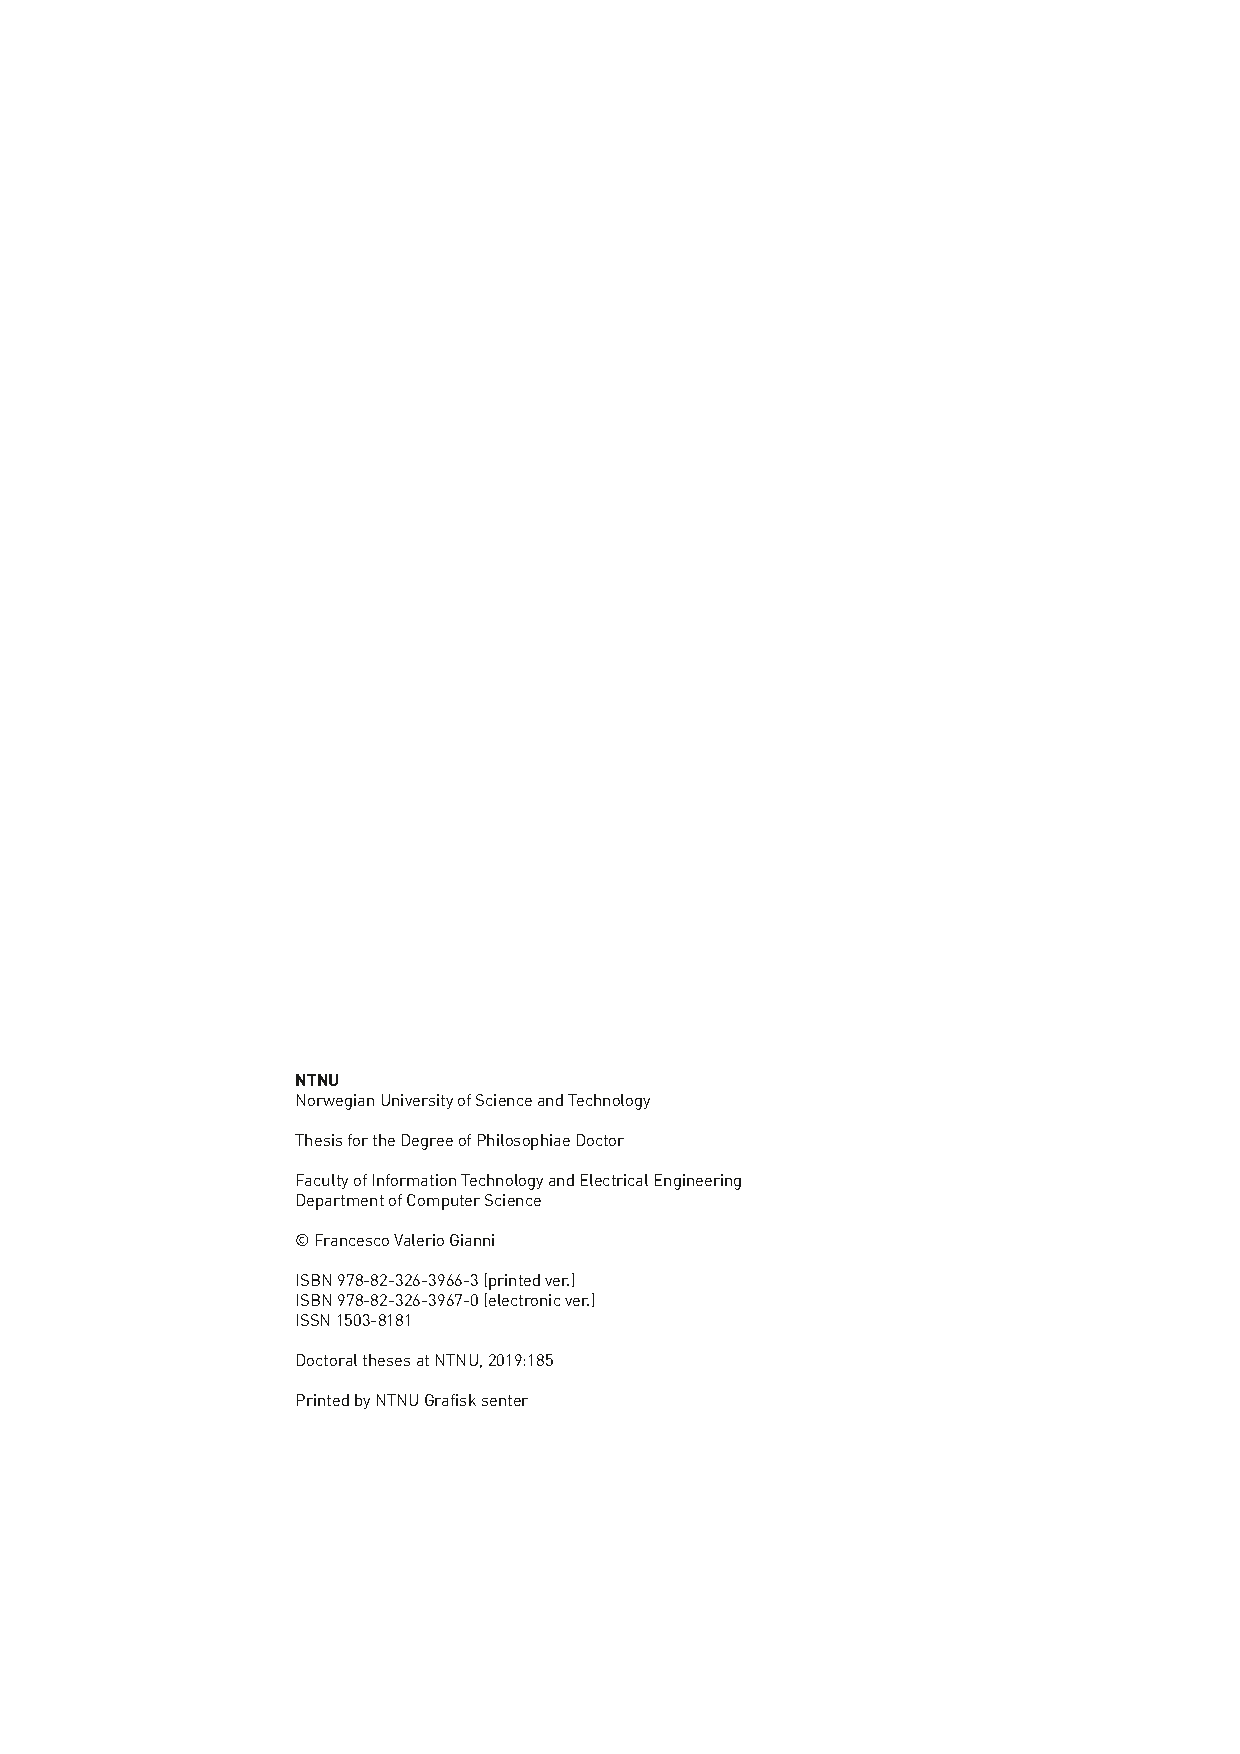
\includepdf{title_page_2.pdf}
\frontmatter
\setcounter{page}{3}
\chapter[Quotes]{}


% \hspace{0pt}
% \vspace{3cm}
% \begin{center}
%     \Large{\textit{\enquote{You Improvise,\\You Adapt,\\You Overcome}}}\\
%     \vspace{1cm}
%     \normalsize{Clint Eastwood --- Heartbreak Ridge, 1986}
% \end{center}
% \vfill
% \hspace{0pt}

\hspace{0pt}
\vspace{34mm}
\begin{center}
\addtolength{\tabcolsep}{-6.6pt} 
\begin{tabular}{rl}
  \Large{\textit{`}} & \Large{\textit{You Improvise,}} \\
    & \Large{\textit{You Adapt,}} \\
    & \Large{\textit{You Overcome'}} \\
\end{tabular}
\addtolength{\tabcolsep}{6.6pt}
\end{center}
\vspace{1pt}
\begin{center}
\normalsize{Clint Eastwood --- Heartbreak Ridge, 1986}
\end{center}
\vfill
\hspace{0pt}

\cleardoublepage
\chapter{Abstract}

Interacting with computers, for work or for leisure, originally required humans to \textit{speak the language of the machine}, intended as interaction techniques, languages and procedures that are closer to how a computer works rather than how the human brain functions. Nowadays, despite the wide availability of computers, this gap is still present. It is now easier to use computers; however, programming even simple applications is still a task approachable only through complex jargon, which has little in common with the final scope of the application.
By addressing the Internet of Things (IoT), we found that this situation is complicated by the involvement of electronics, microcontrollers and low-level programming languages. Specific professional skills are often required to develop and prototype IoT applications.
Research on human-computer interaction (HCI) addresses the challenges of interconnecting people and computers, building tools and theories to facilitate the many uses that a computer can have, in an open-ended dialogue. Thanks to research in this field, new solutions and interaction strategies allowed us to improve user experience when dealing with computers. However, owing to the complexity of the field, in IoT, it is still challenging to keep humans in the loop, in terms of both the development of IoT applications and their use. Specific branches in HCI aim to facilitate the programming phase of computer applications; however, despite being simple, such process still requires the user to have some non-trivial technical skills and an understanding of the basic logical constructs common to most programming languages.

In this thesis, I address how to empower new audiences in brainstorming, designing, programming and prototyping applications for IoT. Some of the already established research fields, such as end-user development (EUD), HCI, interaction design (ID) and software engineering, have already investigated some of these challenges. In this thesis, I will restrict the domain to a specific subset of IoT applications based on tangible user interfaces (TUIs) and smart objects, also covering the phases of brainstorming and design of such applications. Particular focus will be placed on promoting smart city learning (SCL) through the IoT applications envisioned. SCL explores how citizens can be actively involved in a learning process that occurs in the city, making use of its data and services, in order to increase awareness and lifelong learning. The SCL application domain was chosen since it can benefit from IoT technologies, promoting inclusion and participation. In fact, IoT is scarcely used in applications for SCL, while citizens struggle to contribute actively in the life of the city. In order to achieve this inclusive vision, the entry barriers to technology need to be lowered and an integrated process guiding the users during all the phases of the development process should be devised. In this thesis, I will explore how concepts from design thinking, HCI and user-centred design can be implemented in novel tools and processes to support such goal.

This work is grounded in design science research methodologies. Several prototypes were built during eight design iterations, and field studies have been performed at the end of each iteration, for evaluation and validation against acceptance, usability and impact on the problem at stake. Software and hardware rapid prototyping techniques and open-source and digital manufacturing tools have been largely employed. The results of the evaluations were used for validating the already existing theories in HCI, SCL and IoT and for the development of new constructs. Commercial exploitation of the research outcomes is underway.

The resulting contributions add new knowledge to guide the ideation, design, programming and prototyping of IoT applications for users with limited technical skills, placing particular emphasis on the case of applications for SCL. A holistic framework for IoT has been devised to bootstrap the ideation process and guide the users towards a tangible, programmable prototype of the application idea. The work described in this thesis includes the implementation of two toolkits for ideation, programming and physical prototyping. This development task required a wide range of competencies in design, software and hardware engineering. The lessons learned from the experience of the author provided knowledge connected to the creation of tools to ease idea generation and rapid prototyping of IoT applications.

\cleardoublepage
\chapter{Preface}

This thesis was submitted to the Norwegian University of Science and Technology (NTNU) for partial fulfilment of the requirements for the degree of philosophiae doctor.

The main body of doctoral work has been performed at the Department of Computer Science, NTNU, Trondheim, Norway. Professor Monica Divitini was the main supervisor, and Professor John Krogstie and Dr Simone Mora were the co-advisers.
\cleardoublepage
\chapter{Acknowledgements}
\enlargethispage{\baselineskip}

Most of all, I would like to express my deepest gratitude to my supervisor Professor Monica Divitini. You have always been present and supportive for me. Under your guidance I grew up as a researcher and as a person. Thanks for the patience and the effort you dedicated to me.

I am extremely grateful to my co-advisors Professor John Krogstie and Dr. Simone Mora. You have been an example of integrity and professionalism, I was inspired by your hard work and always found support and advice when in need.

I wish to thank all the colleagues and co-authors in our research group who contributed to my work: Anna, Lisa, Mikael and Dag Rune.

I extend my gratitude to the colleagues from the Department of Computer Science and the ISSE group, especially to my mates Elena, Stefano, Massimiliano and Sofia for the engaging and constructive discussions.

Thanks to all my friends in Norway and in Italy for always being supportive, curious and creative, you inspired me to strive for more.

Thanks to my family: Valeria, Massimo, Matteo, Daniele, and to my grandparents Piero, Piera, Cesi e Ugo. Without you all of this would not have been possible, each of you built a piece of who I am today.

A big thank you to Cesilie, who had the rare privilege of being the one to stand \textit{grumpy}-me, \textit{late-working}-me and \textit{ranting}-me. Thanks for patiently listening, for always having helpful words and for the hugs of encouragement.

\begin{flushright}
\emph{\small Francesco Gianni}\\\emph{\small \today}
% February 26th, 2019}	
\end{flushright}

\cleardoublepage
\tableofcontents
\cleardoublepage
\listoffigures
\cleardoublepage
\listoftables
\cleardoublepage
\chapter{Abbreviations}\label{abbreviations}

\textbf{NTNU} Norwegian University of Science and Technology

\textbf{ICT} Information and Communication Technologies

\textbf{UCD} User Centred Design

\textbf{API} Application Programming Interface

\textbf{DSL} Domain Specific Language

\textbf{IDE} Integrated Development Environment

\textbf{I/O} Input/Output

\textbf{W3C} World Wide Web Consortium

\textbf{CSRL} Computer Supported Reflective Learning

\textbf{HCI} Human-Computer Interaction

\textbf{ID} Interaction Design

\textbf{IoT} Internet of Things

\textbf{M2M} Machine to Machine

\textbf{GUI} Graphical User Interface

\textbf{TUI} Tangible User Interface

\textbf{IP} Internet Protocol

\textbf{SCL} Smart City Learning

\textbf{EUD} End-User Development

\mainmatter
\part[Part I]{Introduction and Methods}
\chapterstyle{southall}
\pagestyle{ruled}
\mainmatter

\chapter{Introduction}
\label{cha:introduction}

\section{Domain}
\label{sec:domain}

In this section the research domain of the thesis and the target user group are presented, and a brief description will introduce the adopted concepts of the \textit{Internet of Things} \textit{(IoT)}, \textit{smart cities} and \textit{non-expert} users.


\subsection{Internet of Things}
\label{sec:iot-domain}

Connected objects and appliances appeared as early as in 1982, with the first connected coke machine developed at Carnegie Mellon University. Since then, many definitions have been proposed for IoT \autocites{ashton_that_2009}{gubbi_internet_2013}, while a few basic principles still stand at the foundation and are shared among most of the theoretical interpretations:
\begin{itemize}
	\item Computers are no longer objects, but accessories that can be embedded or placed in the environment, deploying computational power away from the desktop or the server room.
	\item IoT devices have a connected nature. They can share and receive data from each other or communicate over the internet.
	\item Computers are now capable of sensing and acting in the physical world, which goes beyond the traditional computer paradigm of mice and keyboards as input devices and screens as output devices.
\end{itemize}

Some of the proposed definitions are connected to the use of particular technological approaches \autocite{welbourne_building_2009}, whereas others are related to the domain or how the technology is used. A few examples involve machine-to-machine (M2M) systems, networks of sensors to collect data on a territory \autocite{murty_citysense_2008} and technology-augmented appliances designed for a particular domain like households \autocite{alkar_internet_2005} or cities \autocite{hernandez-munoz_smart_2011}. 

In my research, I focused on IoT as an approach to \textit{object augmentation}, as a technological medium to enable the creation of \textit{smart objects}. Given the exploratory nature of the research work performed, energy efficiency, security and cost-reduction aspects related to IoT were addressed with a low level of priority. Forms of IoT outside the notion of smart objects, like the above-mentioned sensor networks, screen-based appliances and IoT applications that do not foresee any user involvement, remained outside of my research domain. 

Smart objects appear and can be used like a regular object, but at the same time they provide additional affordances, thanks to their embedded technological layer. They have been previously defined by Michael Beigl and his colleagues as \enquote{\textit{everyday artefacts augmented with computing and communication, enabling them to establish and exchange information about themselves with other artefacts and/or computer applications}} \autocite{beigl_mediacups_2001}.
This approach to IoT through smart objects enables the creation of \textit{tangible user interfaces} (TUIs) \autocite{ishii_tangible_1997}, a method to interact with a computer application using object manipulation instead of a keyboard and to use output feedback involving several senses instead of a screen.


\subsection{Non-Expert Users}
\label{sec:non-experts}

During my research, the technological approach I embraced was based on a user-centred perspective, thus promoting inclusion and participation, extending the impact of the solutions to a wide portion of the population. I addressed a precise target group of users, defined as \textit{non-experts}, who are individuals that do not need to possess professional skills in design, programming languages, electronics or computer networks.

The aim of my work was to directly involve non-experts in designing meaningful IoT applications, through a process tailored to their capabilities, while meeting their needs and desires. The ultimate goal was to provide access to the affordances offered by IoT to new communities, lowering the access barriers and reducing the complexity.


\section{Challenges}

Working with TUIs and smart objects is challenging because building meaningful applications requires skills in multiple domains, like human-computer interaction (HCI), design, programming and electronics. Moreover, works in these fields have traditionally focused on technical facets \autocite{siegemund_context-aware_2004}, whereas HCI aspects received attention only recently \autocite{nelson_user_2005}. Yet, design principles and methods for smart objects that go beyond mere hardware are at the forefront of research exploration \autocite{kortuem_smart_2010}.

Another demanding point is related to the development process: heterogeneous needs from end-users make the development of products and technological solutions increasingly difficult \autocite{von_hippel_user_2001}. Toolkits for innovation address these challenges, allowing end-users to play an active role in product development. Toolkits allow breaking down the design space into atomic tasks and building blocks, which can be more easily recombined allowing \textit{design-by-trial-and-error}, avoiding costly iterations and speeding up the process \autocite{cvijikj_toolkit_2011}.

Despite the simplifications introduced by the use of the toolkits, following a user-centred approach can still be hard. Non-experts belong to a diverse set of categories, characterised by different needs and skills. Collaborative processes can help by stimulating discussions and allowing users to reach a common ground, a shared lingo allowing them to contribute to the design process despite their diversity.


\section{Motivation}
\label{sec:motivation}

Many solutions and toolkits have been proposed to facilitate the development of IoT applications \autocite{udoh_developing_2017}. The technologies supporting this process include software, hardware, electronic devices and networking protocols. Efforts were made to simplify the assembly and programming of electronic devices involving the use of sensors, actuators and network connectivity. On the software side, several organisations have proposed different standards to define a common interface and a shared data model to represent the typical information bits related to a wide number of IoT devices.
Numerous networking protocols were also created, adapted or re-used in the IoT domain to address specific trade-offs involving bandwidth, latency, energy consumption and wireless coverage \autocite{chen_performance_2016}. In terms of hardware, Arduino \autocite{mellis_arduino_2007} started a revolution introducing a platform that allows users with limited electronic skills to wire sensors and actuators to a microcontroller, programmed through a simplified software toolchain compared to approaches traditionally used in embedded programming.
Despite the innovative solutions and significant advancements in these sub-fields, important challenges are still present in each of them, especially when targeting new audiences that might lack the domain knowledge and technical skills traditionally required to start working with the IoT.

For example, despite the numerous standards, data models, interfaces and networking protocols proposed, none of them emerged as a clear winner, providing an open, royalty-free solution on a par with HTTP and HTML for the web \autocite{guinard_building_2016}. In addition, the data models and software libraries proposed only address IoT devices designed to sense and interact with the ambient environment, such as a thermostat, a temperature sensor or a lamp. There is little support for keeping humans in the loop through typical gestures and patterns that characterise human interaction with objects, like touching, shaking, tilting and so on.
On the hardware side, basic electronic skills and knowledge are still required to wire electronic components to an Arduino microcontroller.

Already existing IoT toolkits and frameworks usually focus on facilitating a single aspect of the development process of an IoT application. For example, they assume that the user will continue in such a process by choosing and adopting a software framework to program the application logic for the electronic device assembled, or that the user will solve the network connectivity problem independently. This silo effect is particularly challenging for non-experts, who might lack the critical skills required to address a particular aspect.

With IoT being a loosely defined concept, non-experts often need to start learning about the domain and technology, exploring the solution space while brainstorming a possible application idea. The silo effect can be mitigated by gradually building knowledge, utilising the same abstractions and constructs during all the development phases. This approach helps devise a holistic process rather than an arbitrary selection of tools that are not necessarily designed to work together. A holistic approach can then ease the democratisation of the technology, enabling wider audiences.

The main domain case addressed in this thesis undertakes some of the challenges affecting modern smart cities. In fact, citizens often fall into the definition of non-experts. Few studies have explored how to enable co-design and promote citizen participation through the use of IoT technologies that keep humans in the loop. A high level of participation in acknowledging the problem and developing a technological solution also promotes the appropriation of the idea. The benefits extend to the idea adoption and to the achievement of a learning impact that lasts longer, compared to prescriptive methods.


\section{Problem Statement}
\label{sec:problem-statement}

The goal of my work was to find new ways to empower non-experts in the development of IoT applications. This was framed as a holistic and creative process, which also aimed to promote lifelong learning and awareness about opportunities and challenges affecting modern smart cities. Smart city learning (SCL) was used as a case and as an application domain. It helped the users find design constraints and goals while at the same time providing a playground to tackle widely recognised societal challenges affecting citizens worldwide. For my research, SCL has demonstrated to be a compelling domain case since (i) citizens often belong to the non-expert user category, (ii) IoT and smart objects can help support lifelong learning, (iii) SCL keeps a user-centred perspective and (iv) it addresses challenges affecting a wide portion of the population.

Analysing the literature on the technological applications for SCL, we discovered a lack of research regarding the following:

\begin{itemize}
\item The use of IoT, tangible interfaces and smart objects, defined in Section~\ref{sec:domain}. Most applications make use of smartphones or screen-based interfaces or do not require direct user interaction with the technology.

\item The role of smart cities as an evolving community of citizens that cooperate and learn continuously to solve challenges related to large urbanisation. Research on smart cities is often limited to confined sub-domains or restricted communities.

\item Active engagement of the users and co-design in the city. Users are often only marginally involved in the studies, resulting in a little impact in terms of learning, long-term behaviour change or awareness of the city challenges.

\item When addressing behaviour changes, the methodologies employed could not convey knowledge or awareness or enrich the user in any way. Most of the times, prescriptive methodologies such as persuasion were used. These methods have limited potential in stimulating the learning outcome and, as such, achieving results that last in time.
\end{itemize}

The tools, theories and technological artefacts adopted during my PhD explored the opportunities at the intersection of the above-mentioned fields. The solutions envisioned follow the principles detailed here:

\begin{itemize}
\item \textbf{IoT} - Technological applications make use of augmented objects and tangible interfaces. Those applications orchestrate the use of ecologies of different interconnected objects. Such objects support the user experience and the application objective by providing immediate sensory feedback, detecting user interaction and collecting environmental data, while being able to communicate with Internet services and data providers.

\item \textbf{SCL} - The domain of smart cities is seen from a user-centred perspective. Several challenges affecting the world population living in cities have been identified by the United Nations \autocite{un_smart_2015}. These challenges were proposed as domain problems to non-expert users, providing a design goal for the IoT applications to be created.

\item \textbf{Co-Design} - The envisioned process extends the involvement of the users beyond the simple usage of the application, addressing also the development phase. Given the potential complexity of the IoT and the non-expert nature of the target users, supporting co-design in this context is particularly challenging.

\item \textbf{Behaviour Changes and Lifelong Learning} -  The IoT applications created by the users during co-design activities are designed to support lifelong learning. Behaviour changes are encouraged and focus on reflective learning and increased awareness. Learning also includes knowledge about the domain and the technologies, which is conveyed while brainstorming and designing the IoT application. These methods better promote a long-term impact and a more permanent outcome, in relation to the specific problems or challenges addressed.
\end{itemize}


\section{Research Methodology}
\label{sec:research-methodology}

The research methodology adopted is based on \emph{design science research} \autocites{hevner_design_2010}{march_design_1995}. Exploratory studies were conducted mainly in the form of design and prototyping workshops, following a \emph{user-centred approach} \autocites{maguire_methods_2001}{gulliksen_key_2003}. During these activities, theories and tools developed during multiple iterations were validated on the field. Co-design was used as a strategy to pursue collaboration, awareness and a long-term impact for the end-users.

Quantitative and qualitative research methods \autocite{robson_real_1993} have been adopted, including observations of the activities of the end-users during the studies. Quantitative data were collected in the form of questionnaires and through a systematic analysis of the artefacts produced by the users. During the studies, the users also produced scenarios, personas, storyboards and public pitch of ideas. These user-generated materials aided the user-centred design work of improvement and refinement of the tools and methods employed. Consistent with the design science research methodology, grounded in the activities of \emph{building} artefacts for a specific purpose and of \emph{evaluating} how well the artefacts perform \autocite{march_design_1995}, a number of prototyping iterations and evaluation studies have been performed on the tools employed during the user studies.

Prototyping involved the construction of a set of tools and technologies supporting the various stages of the development process of an IoT application. The design of such tools was grounded in relevant theories and refined by the experience matured during the user studies, which also contributed to the validation of theories and to the development of new constructs. The numerous user studies performed facilitated building and understanding the domain. I did not have any previous knowledge of design methods and had limited knowledge of electronic prototyping.

All the tools produced were evaluated during studies with the end-users; some of the tools went through multiple iterations. The goal was to assess the utility, usability and efficacy.


\section{Research Questions}
\label{sec:research-questions}

The main research question for my PhD work is as follows:
\begin{quote}
	\textbf{MRQ:} \MRQ 
\end{quote}

In order to answer the main research question, this work was broken down into three sub-questions:
\begin{quote}
	\textbf{RQ1:} \RQi 
\end{quote}
\begin{quote}
	\textbf{RQ2:} \RQii 
\end{quote}
\begin{quote}
	\textbf{RQ3:} \RQiii
\end{quote}


\section{Research Outcomes}

Seven research papers published in peer-reviewed conferences and journals explored the research questions. Building on the results reported in these papers, a body of knowledge regarding the research questions in the fields of SCL, interaction design (ID), HCI and IoT has been developed.

Finally, actions were taken to publicly release the solutions developed, while research contributions were evaluated for commercial exploitation. More information regarding these matters is provided in Section~\ref{sec:exploitation}.


\subsection{Research Papers}
\label{sub:research-papers}

The research questions are addressed in the following research papers:

\begin{enumerate}[label=\numberingI{\textbf{P\arabic*}}]
    \item Gianni, Francesco, and Monica Divitini (2016) \textbf{\enquote{Technology-Enhanced Smart City Learning: A Systematic Mapping of the Literature.}} \emph{Interaction Design and Architecture(s) Journal - IxD\&A} 27:28--43.
    \item Mora, Simone, Francesco Gianni, and Monica Divitini (2017) \textbf{\enquote{Tiles: A Card-Based Ideation Toolkit for the Internet of Things.}} In: Proceedings of the 2017 Conference on Designing Interactive Systems. DIS 2017. 587--598. Edinburgh, United Kingdom: ACM.
    \item Gianni, Francesco, and Monica Divitini (2018) \textbf{\enquote{Designing IoT Applications for Smart Cities: Extending the Tiles Ideation Toolkit.}} \emph{Interaction Design and Architecture(s) Journal - IxD\&A} 35:100--116.
    \item Gianni, Francesco, Lisa Klecha, and Monica Divitini (2019) \textbf{\enquote{Tiles-Reflection: Designing for Reflective Learning and Change Behaviour in the Smart City.}} In: The Interplay of Data, Technology, Place and People for Smart Learning. SLERD 2018. \emph{Smart Innovation, Systems and Technologies} 95:70--82. Aalborg, Denmark: Springer, Cham.
    \item Mavroudi, Anna, Monica Divitini, Francesco Gianni, Simone Mora and Dag R. Kvittem (2018) \textbf{\enquote{Designing IoT Applications in Lower Secondary Schools.}} In: Proceedings of IEEE Global Engineering Education Conference. EDUCON 2018. 1120--1126. Tenerife, Spain: IEEE.
    
    {\footnotesize \textit{
\includegraphics[height=13pt]{trophy.eps} -- Best Paper Award at EDUCON 2018.}}
    \item Gianni, Francesco, Simone Mora, and Monica Divitini (2018) \textbf{\enquote{RapIoT Toolkit: Rapid Prototyping of Collaborative Internet of Things Applications.}} \emph{Journal of Future Generation Computer Systems.} Elsevier.
    
    {\footnotesize \textit{
\includegraphics[height=13pt]{trophy.eps} -- The conference version of this paper received the Best Paper Award at the International Conference on Collaboration Technologies and Systems (CTS) in 2016.}}
    \item Gianni, Francesco, Simone Mora, and Monica Divitini (2018) \textbf{\enquote{Rapid Prototyping Internet of Things Applications for Augmented Objects: The Tiles Toolkit Approach.}} In: Ambient Intelligence. AmI 2018. \emph{Lectures Notes in Computer Science.} 11249:204--220. Larnaca, Cyprus: Springer, Cham.
\end{enumerate}

Table \ref{tab:rq-papers-relation} shows the mapping between research papers and research questions.

\begin{table}
	[tbh] \centering \caption{Connection between research papers and research questions.} \label{tab:rq-papers-relation}
	\begin{tabular}
		{cccccccc} \toprule  & P1 & P2 & P3 & P4 & P5 & P6 & P7 \\
		\midrule 
		RQ1 & & \textbullet & \textbullet & & & \textbullet & \textbullet \\
		RQ2 & \textbullet & \textbullet & \textbullet & \textbullet & \textbullet & &  \\
		RQ3 & & & & & & \textbullet & \textbullet \\
		\bottomrule
	\end{tabular}
\end{table}


\subsection{Research Contributions}
\label{sub:research-contributions}

The seven papers published added to the following contributions:

\begin{quote}
	\emph{\textbf{C1:} \Ci.} This presents challenges and lessons learned derived from the field experience of the author in designing and evaluating a toolkit to support such process.
\end{quote}
\begin{quote}
	\emph{\textbf{C2:} \Cii.} This includes the evaluation, refinement and specialisation of the toolkit to better target the SCL domain. 
\end{quote}
\begin{quote}
	\emph{\textbf{C3:} \Ciii.} This includes the design and production of wireless electronic devices, applications for mobile devices and cloud-based software. 
\end{quote}
\begin{quote}
	\emph{\textbf{C4:} \Civ.} This investigates workshops for brainstorming and tangible exploration of IoT ideas as a means to convey knowledge about technology and smart cities.
\end{quote}
\begin{quote}
	\emph{\textbf{C5:} \Cv.} This describes the first draft of an IoT framework supporting applications that involve object manipulation, as well as sensory feedback and data collection. How the framework can be implemented using established standards and open technologies is also described.
\end{quote}


\section{Context of the Work}

The research work presented in this thesis contributed to the development of the Tiles project\footnote{www.tilestoolkit.io}. The goal of this project is to design and manufacture an integrated set of tools to enable new, non-technical audiences to brainstorm, design and prototype IoT applications involving smart objects. Tiles propositions include ease of use, support for multiple design iterations, velocity, rapid feedback loops and user enjoyment.

As a contributing researcher in the Tiles project, I took part in different activities, such as design, implementation, development coordination, revision and evaluation of different tools created in the context of the project.

The tools produced and the data collected during the evaluations were also employed to explore the learning potential of the Tiles approach in educational contexts. This work was conducted thanks to the support from partners in the UMI-Sci-Ed project\footnote{www.umi-sci-ed.eu}, funded by the European Union. The outcomes of such research are valuable for the work described in this thesis, since they provided insights into the ability of the tools created to convey knowledge about IoT and smart cities to children. Such domain knowledge was required to inform the subsequent phases of development of the IoT ideas.

During my PhD period, I co-advised the specialisation project and master thesis of two students who contributed to the Tiles project and to other areas. The co-advising activities resulted in the co-authoring of P4 and two other articles. In addition, I coordinated the development of the mobile application described in P6. The work was performed by a group of students, as part of a semester course on the management of real-world technical projects.


\section{Structure of the Thesis}

The thesis is composed of two parts:

\begin{itemize}
	\item \textbf{Part I} -- presents the introduction to the research work and provides an overview of the background theories, the methods used, the results achieved and the contributions made by the thesis.
	\item \textbf{Part II} -- contains the seven research papers that added to the results of this thesis.
\end{itemize}

The rest of \textbf{Part I} is organised as follows:

\begin{itemize}
    \item \textbf{Chapter \ref{cha:smart-cities}} offers an overview of SCL and motivates its employment as an application domain.

	\item \textbf{Chapter \ref{cha:toolkits}} introduces related work and defines the toolkits for IoT.
	
	\item \textbf{Chapter \ref{cha:iot-framework}} presents and defines the IoT framework embraced in terms of components, design phases and boundaries.
	
	\item \textbf{Chapter \ref{cha:theory}} describes constructs adopted as theoretical underpinning: co-design and the HCI approach based on TUIs.

	\item \textbf{Chapter \ref{cha:research-methodology}} depicts the research method and approach adopted, providing an overview of the user studies conducted and the prototypes built.

	\item \textbf{Chapter \ref{cha:results}} summarises the results of the research papers.

	\item \textbf{Chapter \ref{cha:contributions}} outlines the contributions of the thesis and their relation to the research papers.

	\item \textbf{Chapter \ref{cha:evaluation}} proposes an evaluation of the contributions in relation to the research questions.

	\item \textbf{Chapter \ref{cha:conclusions}} concludes the thesis sketching future research and possible evolution of the tools presented.
\end{itemize}

\textbf{Part II} contains the seven research papers in full length.
\chapter{The Case of Smart City Learning}
\label{cha:smart-cities}

In this chapter, I introduce the domain of \textit{SCL}, used as a case and an application domain. SCL was employed as a strategy to promote sustainability, awareness and lifelong learning about the challenges affecting modern smart cities. It was used as a design goal, proposed by researchers or facilitators, but directly pursued by the users involved in the studies.

In the remaining of the thesis, the technical solutions described in Chapter~\ref{cha:iot-framework} and theoretical frameworks presented in Chapter~\ref{cha:theory} complement the SCL vision by describing how practical applications can be deployed in the field.


\section{Smart Cities}

Nowadays, most of the world's population live in cities. While cities occupy only 2\% of the surface of the world, they are responsible for 75\% of the global energy consumption and 80\% of $CO_2$ emissions. The concept of smart cities arose as a means to foster innovation and technology adoption and develop data networks in urban environments. Smart city applications focus on a wide range of sub-domains like governance and service infrastructure (i.e. smart grids and water management) or on collecting and utilising data. Smart cities are founded on communities of citizens; the social aspect plays an important role in ensuring a meaningful deployment of the technology, which should serve the citizens despite their diversities. 

One of the most cited definitions in this regard is the one advanced by Caragliu, Del Bo and Nijkamp \autocite*{caragliu_smart_2011}, who stated that a city is smart \enquote{\textit{when investments in human and social capital and traditional (transport) and modern (ICT) communication infrastructure fuel sustainable economic growth and a high quality of life, with a wise management of natural resources, through participatory governance}}.

ICT has recently become part of the mainstream debate on urban sustainability as well as urbanisation because of the ubiquity presence of urban computing and the massive use of urban ICT in urban systems and domains \autocite{bibri_smart_2017}. Indeed, data sensing and information processing are being fast embedded into the very fabric of contemporary cities \autocites{batty_smart_2012}{bibri_big_2016}. A large number of advanced technologies are being developed and applied in response to the urgent need for dealing with the complexity of the knowledge necessary for enhancing, harnessing and integrating urban systems and facilitating collaboration and coordination among urban domains in the realm of smart sustainable urban planning and development \autocite{bibri_big_2016}.

The emergence of this new techno-urban phenomenon has been particularly fuelled by what is labelled \enquote{ICT of the new wave of computing}, that is, a combination of various forms of pervasive computing, the most prevalent of which are ubiquitous computing, ambient intelligence (AmI), IoT and sentient computing \autocite{bibri_social_2017}.

In my work, I envision a smart city firstly as a community of citizens that live and move in the urban environment, as part of their daily routine. This vision finds its roots in the work of Hollands \autocite*{hollands_will_2008}, aiming to support regional competitiveness. Technology is seen as an enabling factor, which does not disrupt the activities of the citizens but rather encourages awareness, builds problem-solving skills and supports lifelong learning, towards an improved quality of life.


\section{Citizen Participation}

Despite the volume of research targeting smart cities, citizens, especially young ones, are often included only for symbolic purposes; meaningful inclusion remains an open challenge \autocite{lansdown_realisation_2010}. While conventional methods of public participation like committee groups and public hearings have failed to engage the majority of the public \autocites{roberts_public_2004}{irvin_citizen_2004}, multidisciplinary methods are currently being investigated in order to give voice to citizens and stakeholders through authentic dialogue, building social capital and trust \autocite{innes_reframing_2004}.

Previous research has voiced the need for ICT development and innovation to be linked with sustainable development and, thus, related future investment to be justified by environmental concerns and socio–economic needs, rather than technical advancement and industrial competitiveness \autocite{bibri_smart_2017}.

In essence, there are two mainstream approaches to smart cities: (i) the technology- and ICT–oriented approach and (ii) the people–oriented approach. Specifically, there are smart city strategies that focus on the efficiency and advancement of hard infrastructure and technology (transport, energy, communication, waste, water, etc) through ICT and strategies that focus on the soft infrastructure and people (social and human capital in terms of knowledge, participation, equity, safety, etc) \autocite{angelidou_smart_2014}. Several challenges have been identified, among which to explore the notion of the city as a laboratory for innovation and to develop technologies that ensure informed participation and create shared knowledge for democratic city governance \autocite{batty_smart_2012}. As for the second approach, Neirotti et al. \autocite*{neirotti_current_2014} described smart cities as a means of enhancing the quality of life of citizens. Smart cities entail human and social factors, apart from physical and technological factors \autocite{galan-garcia_accelerated-time_2014}. Lombardi et al. \autocite*{lombardi_advanced_2012} emphasised additional soft factors such as participation, safety and cultural heritage.

Local city governments are currently investing in advanced ICT to provide technological infrastructures supporting AmI and UbiComp, as well as to foster respect for the environmental and social responsibility \autocite{solanas_smart_2014}. In order to facilitate participation and inclusion under these premises, situated engagement might help by increasing the awareness of the participants regarding the challenges and opportunities of the urban environment where they live and work.

\section{Learning}

The process aiding citizen participation is also a process of learning, improving environmental awareness, knowledge and personal skills \autocite{wilks_voice_2013} and teaching people how to negotiate and respect each other's views \autocite{corsi_child_2002}. 

Smart cities are a recognised eco-system for learning. SCL aims to support the improvement of all key factors contributing to the regional competitiveness of cities: mobility, environment, people, quality of life and governance \autocite{hollands_will_2008}. This approach aspires at optimising resource consumption and saving time, improving flows of people, goods and data\footnote{www.mifav.uniroma2.it/inevent/events/sclo/}.
Data produced in the city, social challenges affecting the population and technologies are all taken into account and used to increase awareness and lifelong learning through technological applications where citizens represent active actors.


\section{Technology}

Technology is a fundamental component of smart cities. Through technology, urban data can be collected, aggregated and analysed to extract valuable information. Digital solutions can also help lower the costs and increase the efficiency in many strategic sectors like governance, transportation, infrastructure and social services for the citizens. Urban data can support researchers and decision-makers in discovering the hidden layers of smart cities, highlighting patterns and processes that were otherwise impossible to detect \autocite{vazifeh_addressing_2018}.

IoT plays an important role as an enabling technology for this vision. Sensor networks and M2M systems are largely employed to monitor the city and sense and collect the data generated in the urban environment. In addition to this data-driven approach, ongoing research is also exploring how technology can be used to better connect with the population, reinforcing the social aspect and building a sense of community.


\section{SCL as a Domain Case}

The domain of SCL has been defined in the early phases of my research, when drawing the boundaries for an exploratory study about the state of the art, described in P1. It is important to underline how SCL is an emerging field, a wide umbrella under which the concepts exposed in the previous sections of this chapter partially overlap. SCL addresses all the components of a smart city described above, which represents a specialisation since many smart city applications found in literature do not include for example a learning or participation component. In addition, the criteria defined and employed in P1 include a social and an urban perspective (see P1~\S2.1).
The studies analysed in P1 and considered relevant for the survey conformed to at least one of these two criteria, meaning that on the social perspective they did not exclude any category of citizens and on the urban perspective they were referencing to an environment only to be found in cities. Given the exploratory nature of the literature mapping in P1, some studies that overlapped only partially with the definition of SCL were included in the analysis to provide a comprehensive understanding of gaps and trends in the research field.

The philosophy of SCL and the values it promotes present many points of contact with the social and technological framing described in Chapter~\ref{cha:introduction}. More in particular, SCL is a relevant domain case for my work since it is connected to the following notions:

\begin{itemize}
	\item Citizens as active actors, directly involved in and contributing to the urban environment, instead of being relegated to a passive role.
	\item The urban population as non-expert users, citizens often fit in this category, which represents the target user group for my research.
	\item The paramount role of new technologies, able to keep the user in the loop.
	\item The use of technology as a tool to also promote learning, inclusion and social awareness.
	\item The possibility of creating meaningful technological applications, tackling recognised challenges affecting most of the population.
\end{itemize}

These shared values create both an opportunity to contribute to the SCL domain, by generating new solutions and methods addressing societal challenges affecting cities, and a compelling design space to experiment with innovative technologies.

\chapter[Related Work]{Related Work: IoT Toolkits}
\label{cha:toolkits}


In the HCI field, Greenberg \autocite*{greenberg_toolkits_2007} defined toolkits as a way to encapsulate interface design concepts for programmers, as a language that facilitates creation \autocite{myers_past_2000}. More widespread in the literature is the concept of toolkits as a means to describe various types of software, hardware, design and conceptual frameworks. More articulated definitions based on the original one from Greenberg were subsequently proposed, defining toolkits as generative platforms designed to create new interactive artefacts, provide easy access to complex algorithms, enable fast prototyping of software and hardware interfaces and/or enable creative exploration of design spaces \autocite{ledo_evaluation_2018}. Toolkits can support users via programming or configuration environments consisting of many defined permutable building blocks, structures or primitives, with a sequencing of logical or design flow affording a \textit{path of least resistance} \autocite{ledo_evaluation_2018}. Wobbrock and Kientz \autocite*{wobbrock_research_2016} viewed toolkits as contributing \textit{artefacts}, where \textit{\enquote{new knowledge is embedded in and manifested by artefacts and the supporting materials that describe them}}.

Research on and involving toolkits is considered \textit{constructive research}, defined as \textit{\enquote{producing understanding about the construction of an interactive artefact for some purpose in human use of computing}} \autocite{oulasvirta_hci_2016}. Thus, they are generative platforms designed to create new artefacts, while simplifying the authoring process and enabling creative exploration \autocite{ledo_evaluation_2018}.

Ledo et al. \autocite*{ledo_evaluation_2018} summarised the value of toolkits into five goals:
\begin{itemize}
    \item \textbf{G1} - Reducing Authoring Time and Complexity. Concepts are encapsulated to simplify expertise, making it easier for users to author new interactive systems \autocites{greenberg_toolkits_2007, olsen_jr_evaluating_2007}.
    \item \textbf{G2} - Creating Paths of Least Resistance. Defined rulesets and pathways lead the users to consistent solutions \autocite{myers_past_2000}.
    \item \textbf{G3} - Empowering New Audiences. Thanks to the reduced authoring effort, new audiences can be involved in the authoring process, like artists and designers \autocite{olsen_jr_evaluating_2007}.
    \item \textbf{G4} - Integrating with Current Practices. Existing infrastructures and standards can be leveraged as building blocks, enabling power and robustness in combination \autocite{olsen_jr_evaluating_2007}.
    \item \textbf{G5} - Enabling Replication and Creative Exploration. Implementation and replication of ideas to explore a concept can be the first step to the creation of a new suite of tools \autocite{greenberg_toolkits_2007}.
\end{itemize}

Many of these goals are well adapted to tackle the research objectives presented in Section~\ref{sec:motivation}. For example, G5 promotes the creation of new tools, which can help overcome the lack of human-centred IoT solutions in the SCL domain. G2 and G3 extend the influence to new audiences, directly involving users in the authoring process and facilitating prototyping. This approach suits the co-design methodology and assists the involvement of non-expert users. The reduced authoring time described in G1 allows iterating quickly during hands-on activities, achieving tangible results in less than a day of work.


\section{Common Toolkit Architectures}

Toolkits are typically different from systems that perform a single task (e.g. an algorithm or an interaction technique) as they provide generative, open-ended authoring within a design space \autocite{ledo_evaluation_2018}. They support the creation of different solutions by reusing and combining the building blocks provided. These blocks can take the form of software modules with a simplified interface or hardware components that can be easily recombined or implement other forms of encapsulation and abstractions connected to specific realms like interaction modalities, communication protocols or application domains.
This open-ended, generative authoring process within a domain space differentiates toolkits from systems that perform a single task. Different solutions can be created by recombining and adapting the building blocks provided, through a process significantly quicker and simpler than building a dedicated system.


\section{Card-Based Toolkits for IoT}

During co-design activities, brainstorming cards are often used to promote idea generation \autocite{vaajakallio_design_2014}.
Using cards makes focus change easier \autocite{hornecker_creative_2010}; cards can act as a mediator to the conversation between participants from different backgrounds during creative workshops \autocite{carneiro_io_2011}.
The nature of cards inherently supports non-expert users hiding unnecessary complexities, while playing an informative role. They allow users to brainstorm and explore ideas focusing on the design rather than dealing with technical constraints. During such activities, users can point to, discuss and pass around cards, encouraging collaboration and social interaction and fostering creativity \autocite{carneiro_io_2011}. The outcome of this process is usually a design idea, or the framing of a small project, towards which the users develop a better level of connection and empathy.

Several card-based toolkits supporting brainstorming activities for the IoT can be found in the literature.

\begin{itemize}
    \item IoT service kit\footnote{iotservicekit.com} uses paper maps, 3D printed tokens and cards as artefacts representing the context, domain, assets and interactions. The toolkit supports the framing of several layers of an IoT solution. It is possible to define the needs in terms of technologies, sketch a user journey and map the flow of data.
    \item Mapping the IoT\footnote{mappingtheiot.polimi.it} was created to refine already existing ideas and to support the user in the process of enriching and augmenting through technology existing products. The toolkit promotes a meta-design approach, starting with the definition of the target users, markets and technologies and using these findings as a focus point to define the project brief. The cards contain elements of the design process, technology, context, strategy and interaction techniques.
    \item IoT design deck\footnote{iotdesigndeck.com} covers the brainstorming and design phases of an IoT application through several decks of cards. As a first step, participants define the domain, the target user, the problem and which type of technology to use. Five additional decks of cards are used to inspire the design, propose provocative themes and define the inputs and outputs employed.
    \item IoT ideation cards\footnote{sites.google.com/studiodott.be/research/iot-ideation-cards} is a customisable card deck to conceptualise and define IoT product ideas. The cards can be arranged to compose a storyboard to illustrate logic flows, data networks and use cases. The goal is to allow any kind of team to visualise all the components that play a role in an Internet connect product.
    \item Know cards\footnote{know-cards.myshopify.com} represent simple electronic components, divided into decks representing sensors, actuators, power sources and connectivity. The cards can be used to brainstorm technology-driven applications, to learn about already existing components or to play with ideas involving random cards.
\end{itemize}

These toolkits were a source of inspiration for my work. However, none of them presented all the necessary features to cover my research objectives, described in Section~\ref{sec:motivation}. For example, some of the toolkits are meant to be used by professionals or necessitate direct supervision from design experts to be employed. Others cover only a narrow design space, whereas some of them are meant to be used through a process lasting several days or weeks.

\chapter{The Tiles IoT Framework}
\label{cha:iot-framework}

In this chapter, the concept of IoT adopted in my research is described. The domain is defined by specifying boundaries, recalling the theories embraced and explaining how this scenario was deployed into the \textit{Tiles IoT framework}. The Tiles framework is composed of a set of tools and a process, guiding the users towards the creation of an IoT application. The concepts described in this chapter are reflected in the research work performed during my PhD, but they also extend into future improvements and developments.


\section{Process}
\label{sec:iot-ideation-process}

The process defined by the Tiles IoT framework is designed to guide non-expert users through the creation of an IoT application. It is divided into five \textit{phases}, reported in Fig.~\ref{fig:ideation-process}. The process starts with the problem elaboration phase and finishes with the production of a low-fidelity prototype of the IoT application.
A brief description of the different phases is provided in the following paragraphs.

\begin{figure}[ptb]
    \centering 
	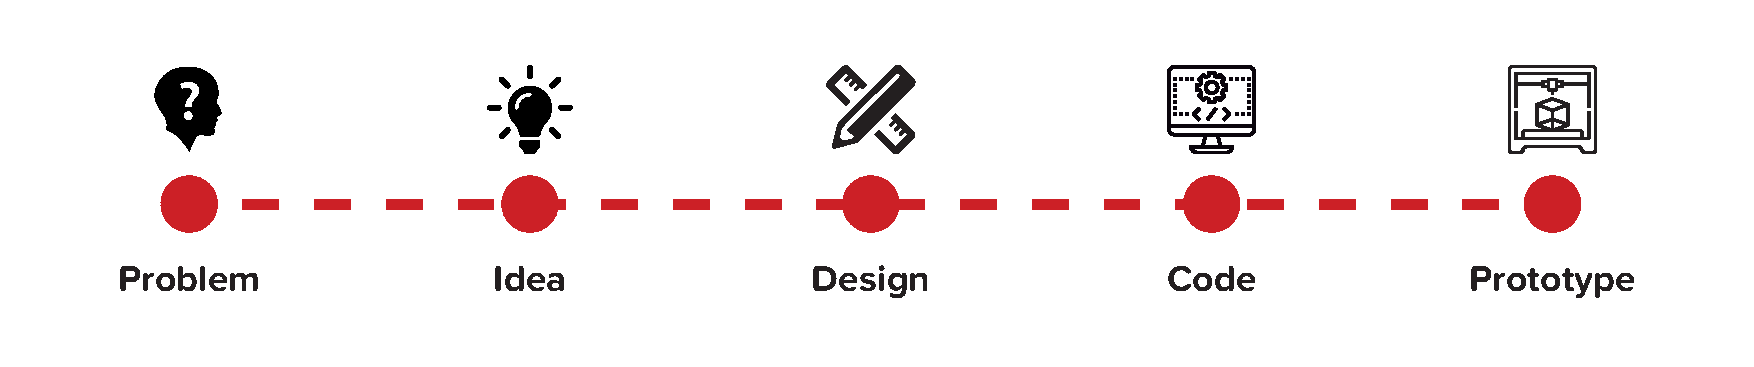
\includegraphics[width=\textwidth]{ideation_process}
	\caption{The process envisioned by the Tiles IoT framework.}
	\label{fig:ideation-process}
\end{figure}

\subsubsection{Problem}
During this first phase, the users select or define a problem that they are willing to address. In order to ease the start of the process, during my work, I often provided the users with a small set of design problems connected to smart cities to choose from.

\subsubsection{Idea}
During this phase, the users combine the different conceptual building blocks that compose a typical IoT application in order to generate smart objects that are relevant to the problem at stake. This brainstorming phase is fuelled by the creativity of the users, who are free to experiment and discuss different solutions and combinations of technology-augmented artefacts. In the papers included in Part II of this thesis and in the remaining of Part I, this phase is referred to as the \textit{brainstorming} or \textit{idea generation} phase.

\subsubsection{Design}
During the \textit{design} phase, the smart objects devised while brainstorming are complemented with a use case scenario. This step guides the users through defining how the objects behave, deciding what the logical connections are among the components of the smart objects and clarifying how the objects interact with each other and with the end-users. The users are also encouraged to reflect on the solution created, analyse it under a different perspective and eventually modify it to match distinct quality criteria.

\subsubsection{Code}
The IoT application design, behaviour and logical connections are translated into code during this phase. I will refer to this phase as the \textit{coding} or \textit{programming} phase throughout the remaining of this thesis.

\subsubsection{Prototype}
The final step consists in physically assembling a low-fidelity prototype of the smart object, which will exhibit the behaviour programmed during the \textit{coding} phase. The prototype created is intended to serve as a physical demonstrator. Efforts are made to improve the speed of development and the possibility of quickly iterating on the implementation, rather than on the complexity of the solution and the long-term stability. I will refer to this phase when discussing \textit{physical prototyping}, \textit{rapid prototyping} or \textit{tangible exploration of ideas} in the next chapters.


\section{Tools}

In order to support the five phases of the Tiles IoT framework process, two toolkits were created from scratch within the Tiles project. When combined, the \textit{Tiles ideation toolkit} and the \textit{RapIoT toolkit} support all the phases of the process defined by the Tiles IoT framework (Fig.~\ref{fig:ideation-process}). The toolkits are composed of an integrated set of technologies and design tools supporting non-experts in a consistent way. The first three phases of \textit{problem elaboration}, \textit{brainstorming} and \textit{design} are supported by the \textit{Tiles ideation toolkit} (see P2, P3 and P4), whereas the last two phases of \textit{programming} and \textit{prototyping} are addressed by the \textit{RapIoT toolkit} (see P6 and P7). A detailed overview of the process in relation to the toolkits is provided in Fig.~\ref{fig:framework}.

\begin{figure}[ptb]
    \centering
	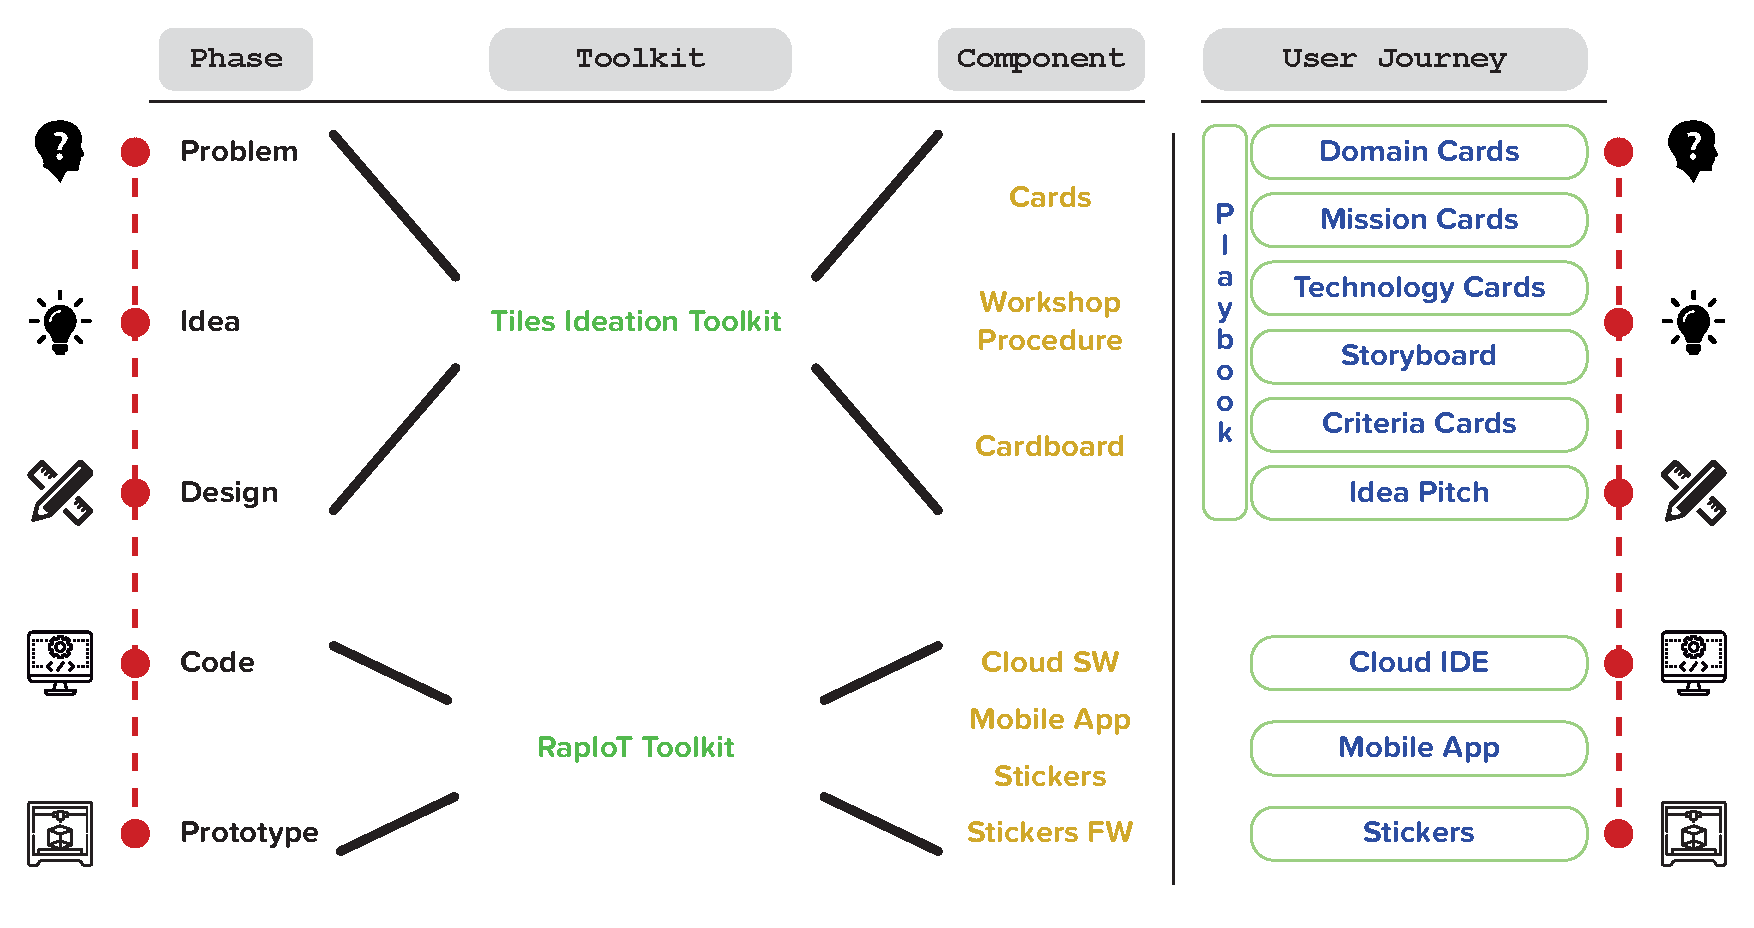
\includegraphics[width=\textwidth]{framework}
	\caption{Mapping of toolkits, components and phases of the Tiles IoT framework.}
	\label{fig:framework}
\end{figure}


The toolkits were designed to support object augmentation as a design strategy for IoT applications. This approach foresees an object as a means of interaction with the \textbf{user} the \textbf{ambient} and the \textbf{network}.

\textbf{User}. When manipulated by the users, augmented objects should be able to sense and distinguish different input commands or gestures (e.g. when a user knocks on, grabs, tilts or shakes an object). As an analogy, similar interaction gestures are widely known and employed in mouse-based interactions (clicking, dragging, double-clicking, etc) and touch interfaces (tapping, double-tapping, swiping, pinching, etc), but they have not been defined for generic object-based interactions.
Augmented objects can also provide sensory feedback and communicate back with the users through actuators, for example, in the form of sound, light or vibration.

\textbf{Ambient}. Objects can sense the ambient where they are positioned and used. Distributed sensing is one of the most popular application domains of IoT. However, in the IoT framework described here, the ability to sense the ambient surrounding the object is not the main function of the object itself. Ambient data like temperature, air pollution and humidity can be used to extend the affordances exposed, enriching the user experience provided by the IoT application.

\textbf{Network}. Connected objects allow integration with services and data streams available on the Internet. Traditionally, IoT applications use networks also to transfer upstream sensor data collected on the field. While these are important use cases that are not discarded by the IoT framework described here, we emphasise the opportunity that a logical \textit{mesh} network topology can offer. A single IoT application can make use of multiple objects that exchange information among themselves. Objects can either sense or provide feedback, or a combination of both. IoT can be more than a network of sensors that only communicates with a central server and presents data through a screen. Ambient sensing, user interaction and feedback are distributed in the environment and interconnected and are part of the same application logic.


\subsection{The Tiles Ideation Toolkit}
\label{sec:tiles-toolkit}

The \textit{Tiles ideation toolkit} (Fig.~\ref{fig:tiles-ideation}) consists of several decks of cards representing the building blocks of an IoT application, a cardboard scaffolding the use of the cards and a workshop technique, which guides the users step by step in the idea generation and design process. The \textit{Tiles ideation toolkit} presents a set of unique characteristics that are not found in already existing card-based toolkits:

\begin{itemize}
    \item \textbf{Velocity}. It allows generating and discussing an idea in less than two hours.
    \item \textbf{Self-containment}. All the materials required are available to the user from the very beginning.
    \item \textbf{Autonomy}. Participants do not need to be supervised or guided by facilitators to complete the creative process.
    \item \textbf{Accessibility}. No technical skills, domain knowledge or design abilities are required.
\end{itemize}

\begin{figure}[ptb]
    \centering 
	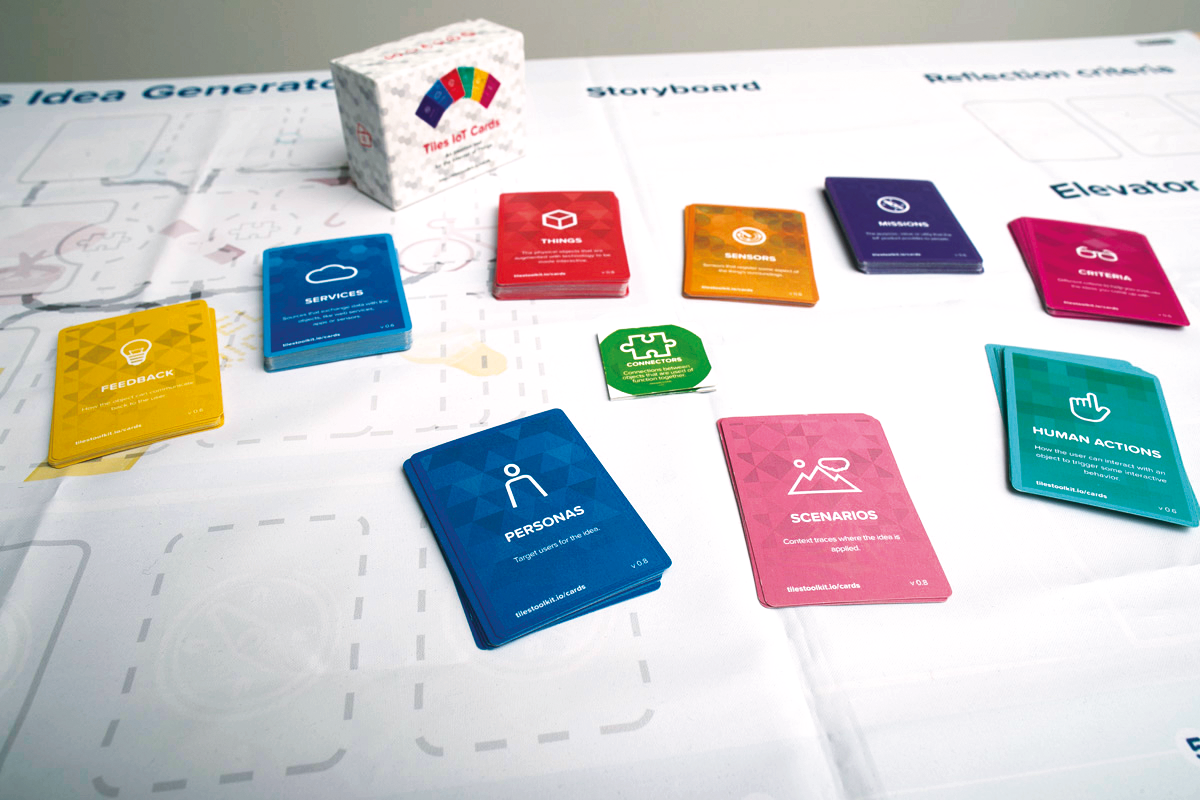
\includegraphics[width=\textwidth]{cards}
	\caption{The last version of the Tiles ideation toolkit. The cardboard and the cards, including the extensions described in P3, are visible in the picture.}
	\label{fig:tiles-ideation}
\end{figure}

In the following I will describe the artefacts and components that constitute the Tiles ideation toolkit. Their relations to the phases of the Tiles IoT framework are also detailed.

\subsubsection{Components}

The phases of \textit{problem elaboration}, \textit{brainstorming} and \textit{design} are addressed by the Tiles ideation toolkit. The workshop technique envisioned by the toolkit is described in detail in the \textit{playbook} visible at the bottom part of the cardboard (Fig.~\ref{fig:cardboard}). The highlighted sectors on the cardboard in Fig.~\ref{fig:cardboard} can be mapped to the first three phases of the Tiles IoT framework process; the cardboard itself and the workshop technique support all the three phases. The individual components of the Tiles ideation toolkit are illustrated in the following.


\begin{figure}[ptb]
    \centering 
	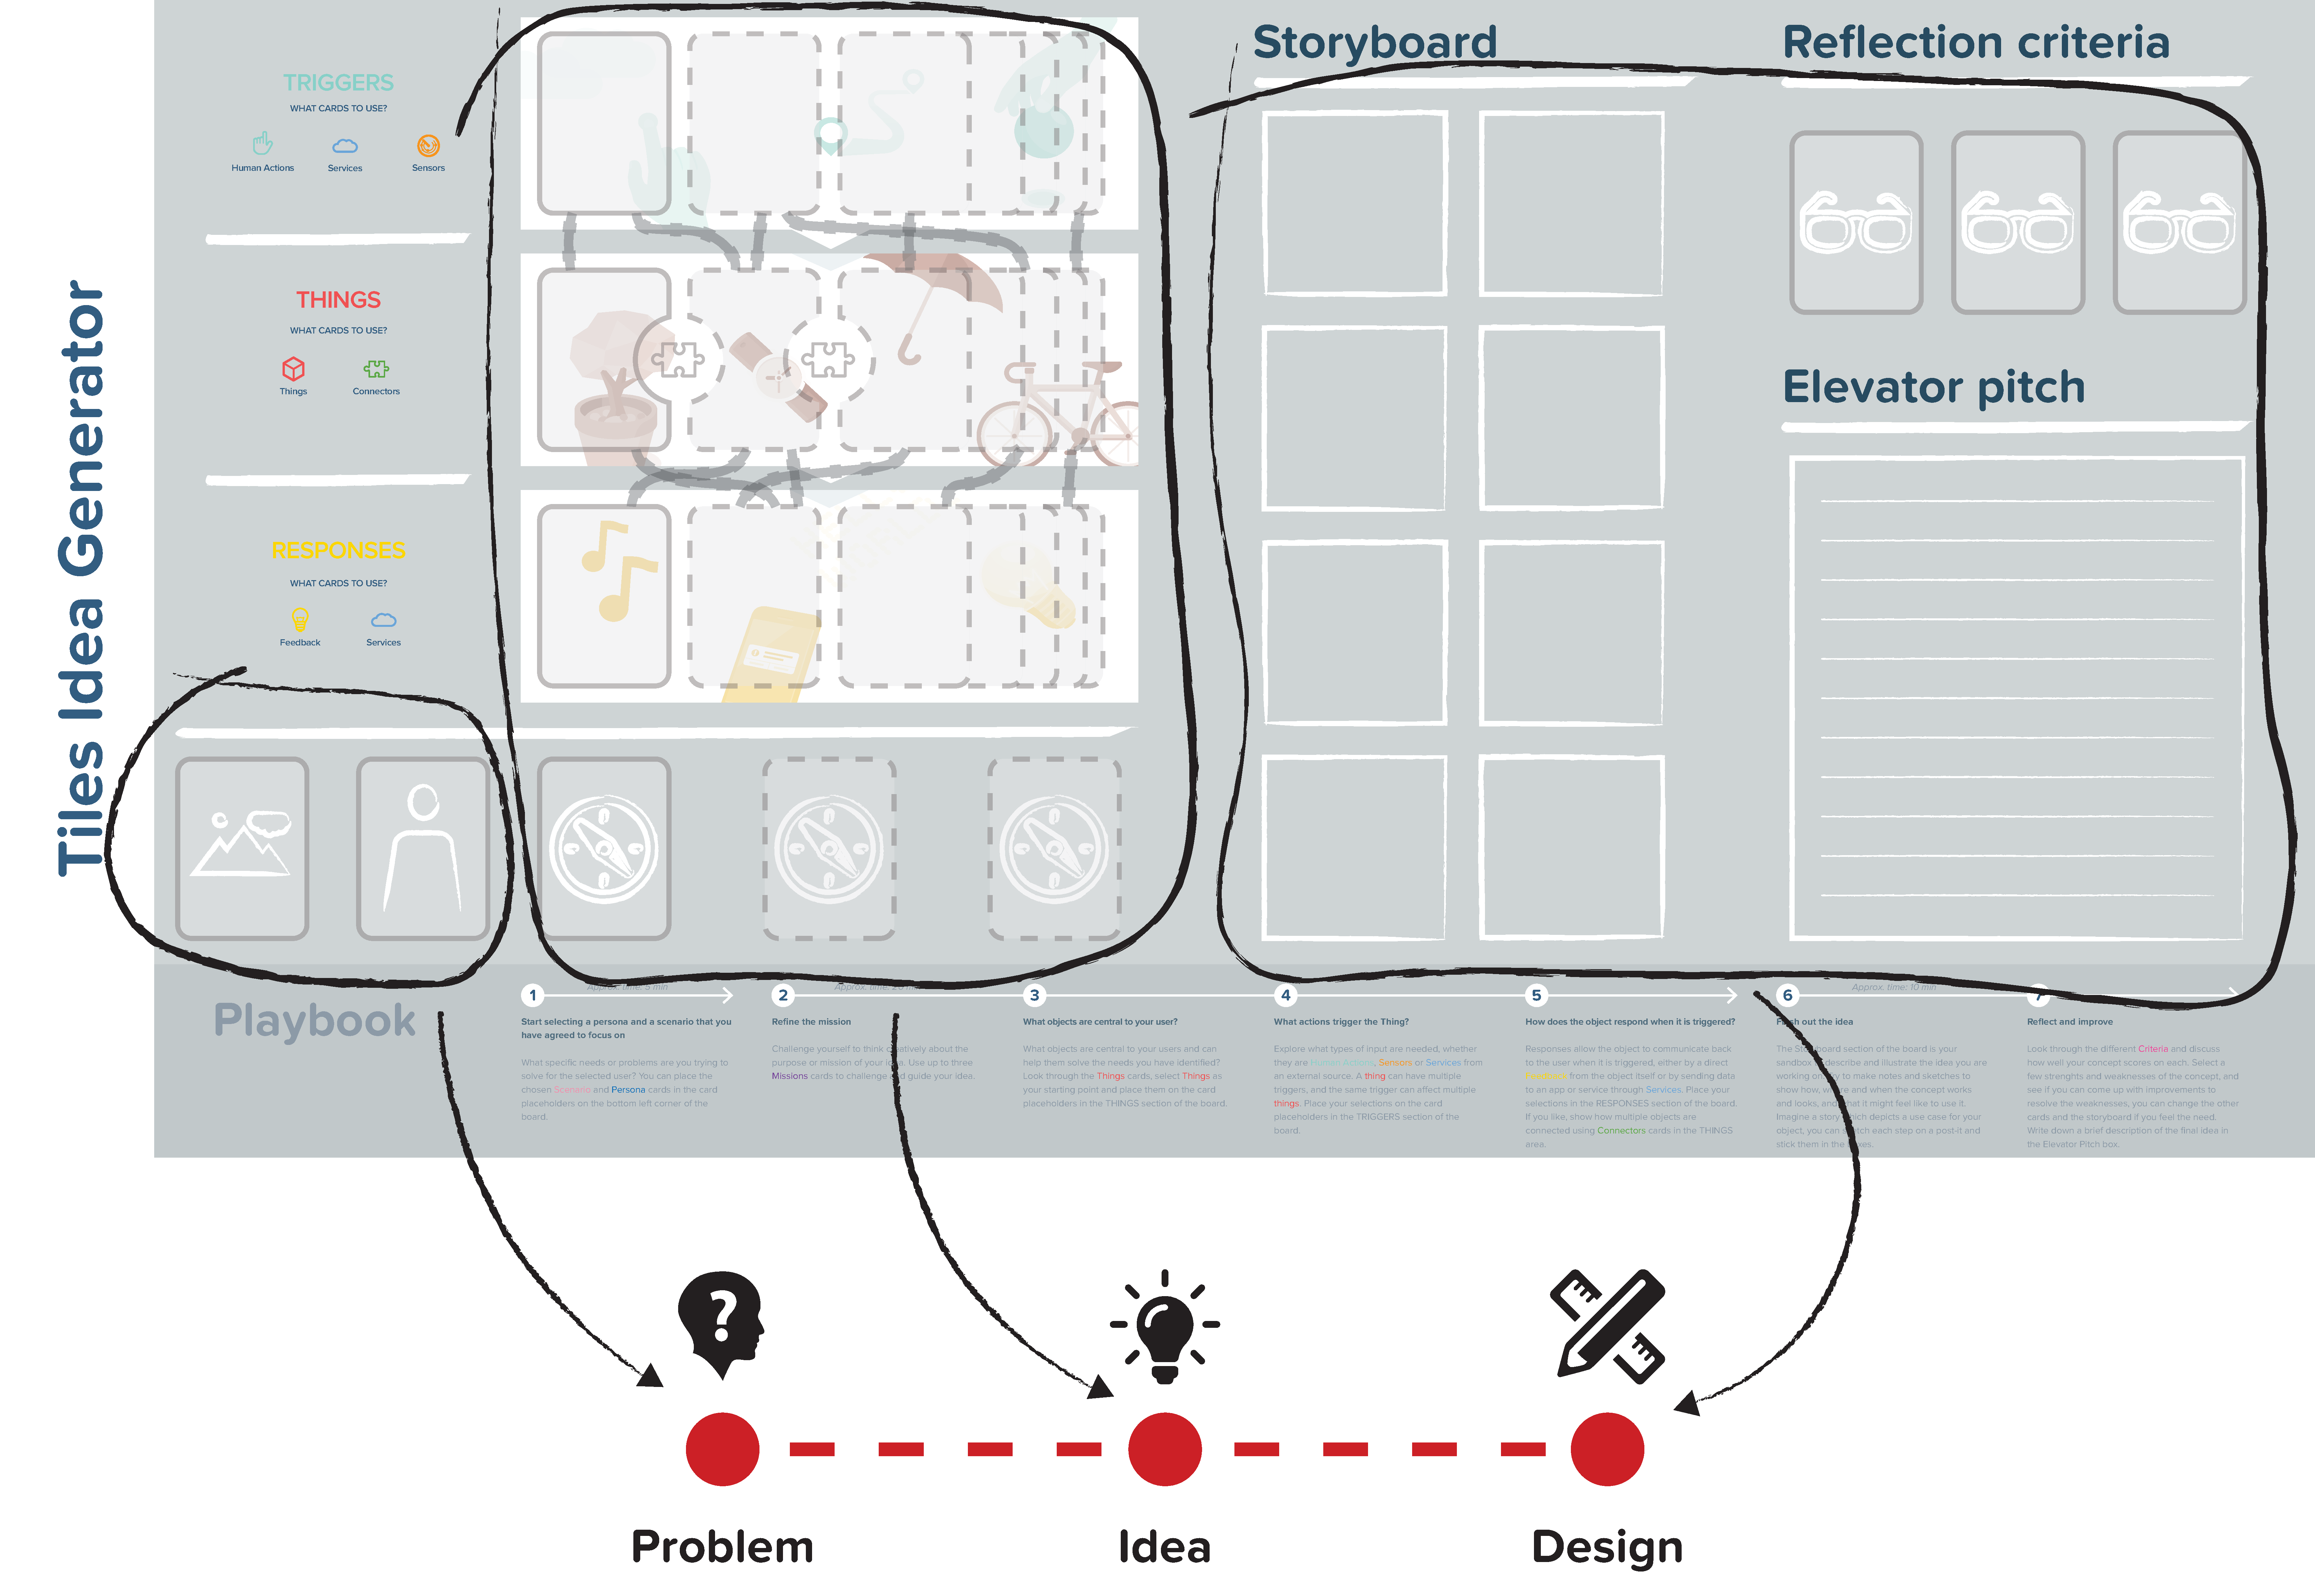
\includegraphics[width=\textwidth]{cardboard}
	\caption{The cardboard included in the Tiles ideation toolkit. The circled sections are connected to the phases of the Tiles IoT framework process.}
	\label{fig:cardboard}
\end{figure}


\textit{\textbf{Personas}} and \textit{\textbf{scenarios}} cards. These cards are used during the initial \textit{problem elaboration} phase, where workshop participants select a target user and a problem to address with their IoT application idea (Fig.~\ref{fig:cards}).

\textit{\textbf{Things}}, \textit{\textbf{sensors}}, \textit{\textbf{services}}, \textit{\textbf{feedback}}, \textit{\textbf{human actions}}, \textit{\textbf{missions}} and \textit{\textbf{connectors}} cards. Workshop participants can define one or more smart objects and model their interactions with the user by combining these decks of cards during the \textit{brainstorming} phase.

\textit{\textbf{Criteria}} cards, \textit{\textbf{storyboard}} and \textit{\textbf{idea pitch}}. In the final \textit{design} phase, workshop participants are encouraged to illustrate a use case for their idea, involving their target user and the augmented objects devised and addressing the problem selected. In order to do that, they sketch a storyboard using post-it notes. The \textit{criteria} cards are also used during this stage to further refine and specialise the idea. Finally, a short text used to pitch the idea is created, thus condensing the ultimate outcome (Fig.~\ref{fig:cardboard}).

For a graphic overview of the final result in terms of creative artefacts and ideas, see the pictures included in P3.

\begin{figure}[ptb]
    \centering 
	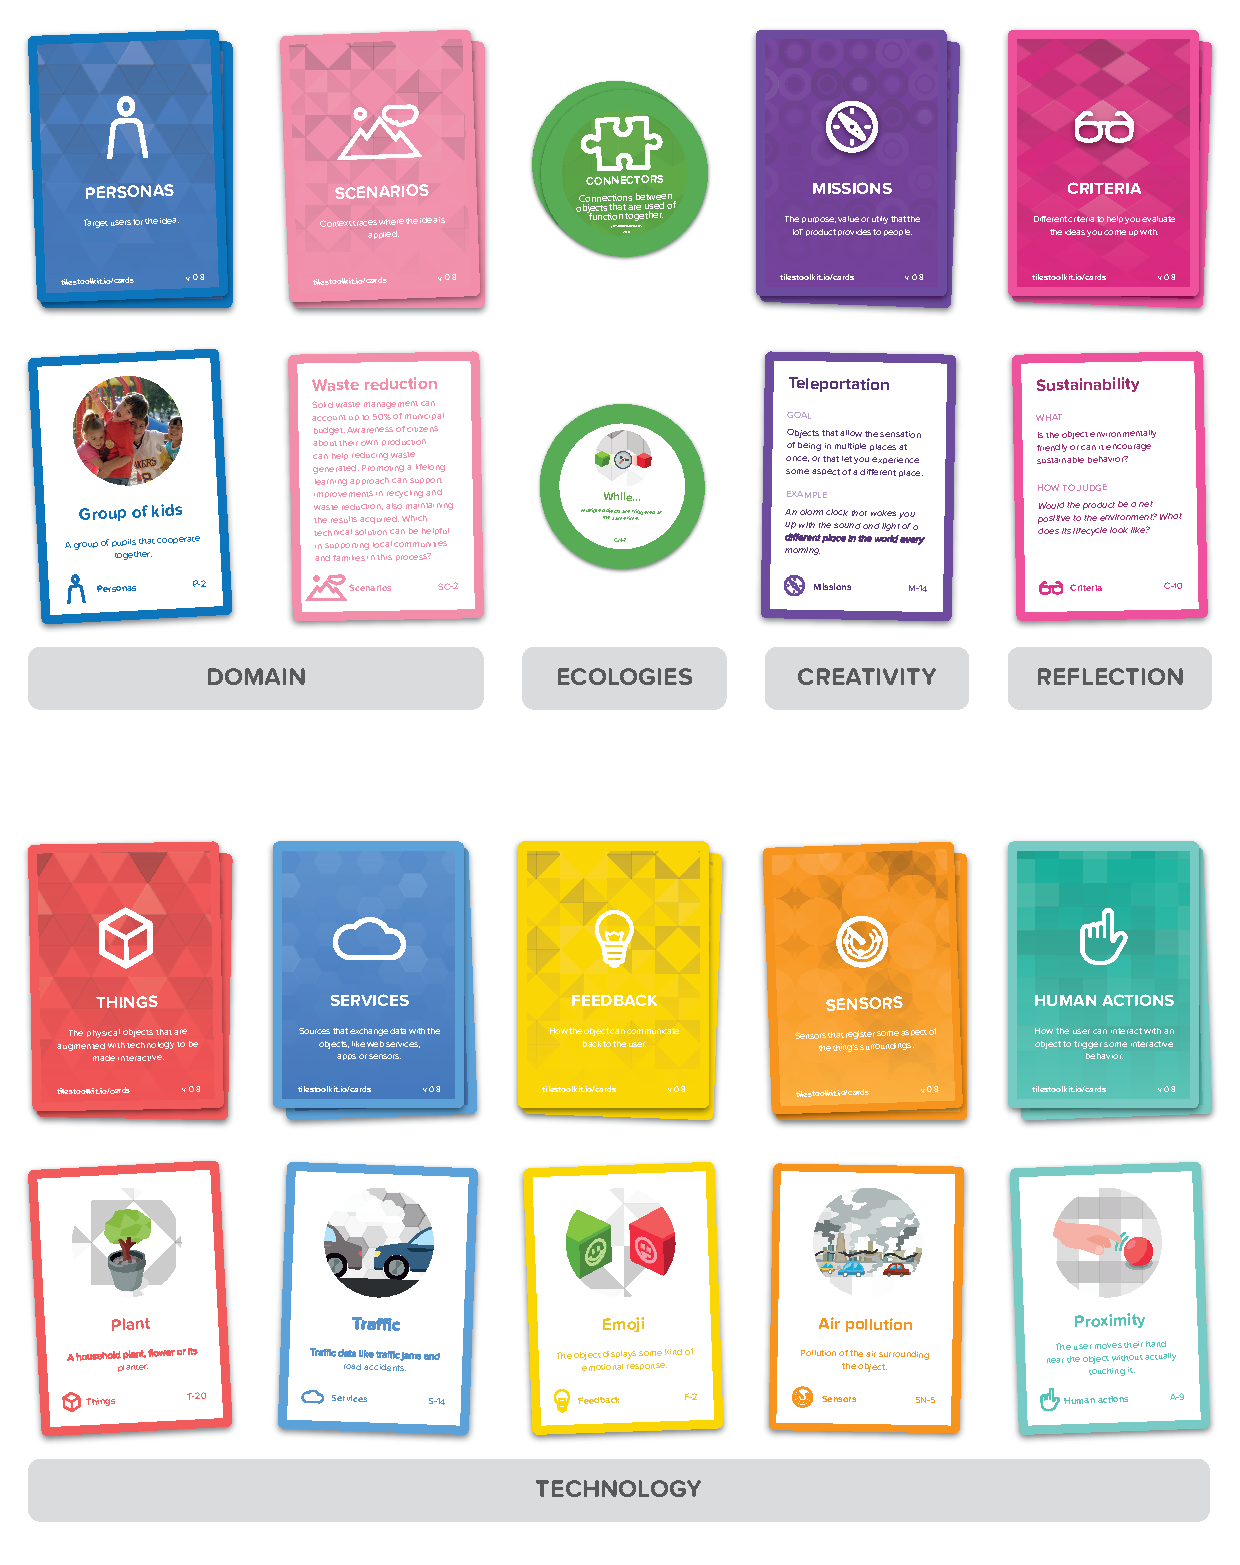
\includegraphics[width=\textwidth]{ideation_cards}
	\caption{Cards included in the Tiles ideation toolkit.}
	\label{fig:cards}
\end{figure}


\subsection{The RapIoT Toolkit}

The \textit{RapIoT toolkit} supports the last two phases of the process defined by the Tiles IoT framework: \textit{coding} and \textit{prototyping} (Fig.~\ref{fig:ideation-process}). These two phases are supported by the use of programmable electronic devices for object augmentation (P7), which function and can be programmed thanks to dedicated software components (P6). Implementing rapid prototyping as object augmentation allows the users to quickly explore the concepts generated during the previous phases. The RapIoT toolkit includes both software and hardware components, allowing the creation of programmable augmented objects.

\subsubsection{Hardware Components}

\textbf{\textit{Stickers}}. As in the other phases, objects remain central and are augmented through electronic \textit{stickers}, which provide sensing and actuation capabilities in a flexible way (Fig.~\ref{fig:stickers}). Modern low-power microcontrollers can be easily embedded in a \textit{sticker} measuring only a few centimetres in length. In a package smaller than 5 x 5 mm, the microcontroller employed includes considerable processing power, communication lines to interact with the attached sensors and actuators and support for secure, IP-based wireless connectivity. These microcontrollers can operate on batteries for years, taking advantage of low-power sleep modes when idle. The \textit{stickers} are battery-powered and connected to the cloud through a gateway, or directly without the need for any other device. Different types of \textit{stickers} can provide different combinations of I/O; many of them can potentially be attached to a single object. They can trigger events while sensing the surrounding ambient or when the users interact with the object that they are attached to. The data packet representing the event is transmitted to the cloud, where the application logic is running. The \textit{stickers} can also consume events received from the cloud (e.g. a command to vibrate). The type and number of events that can be consumed or generated by a \textit{sticker} are only dependent on the type and number of sensors and actuators it has onboard.

\begin{figure}[ptb]
    \centering 
	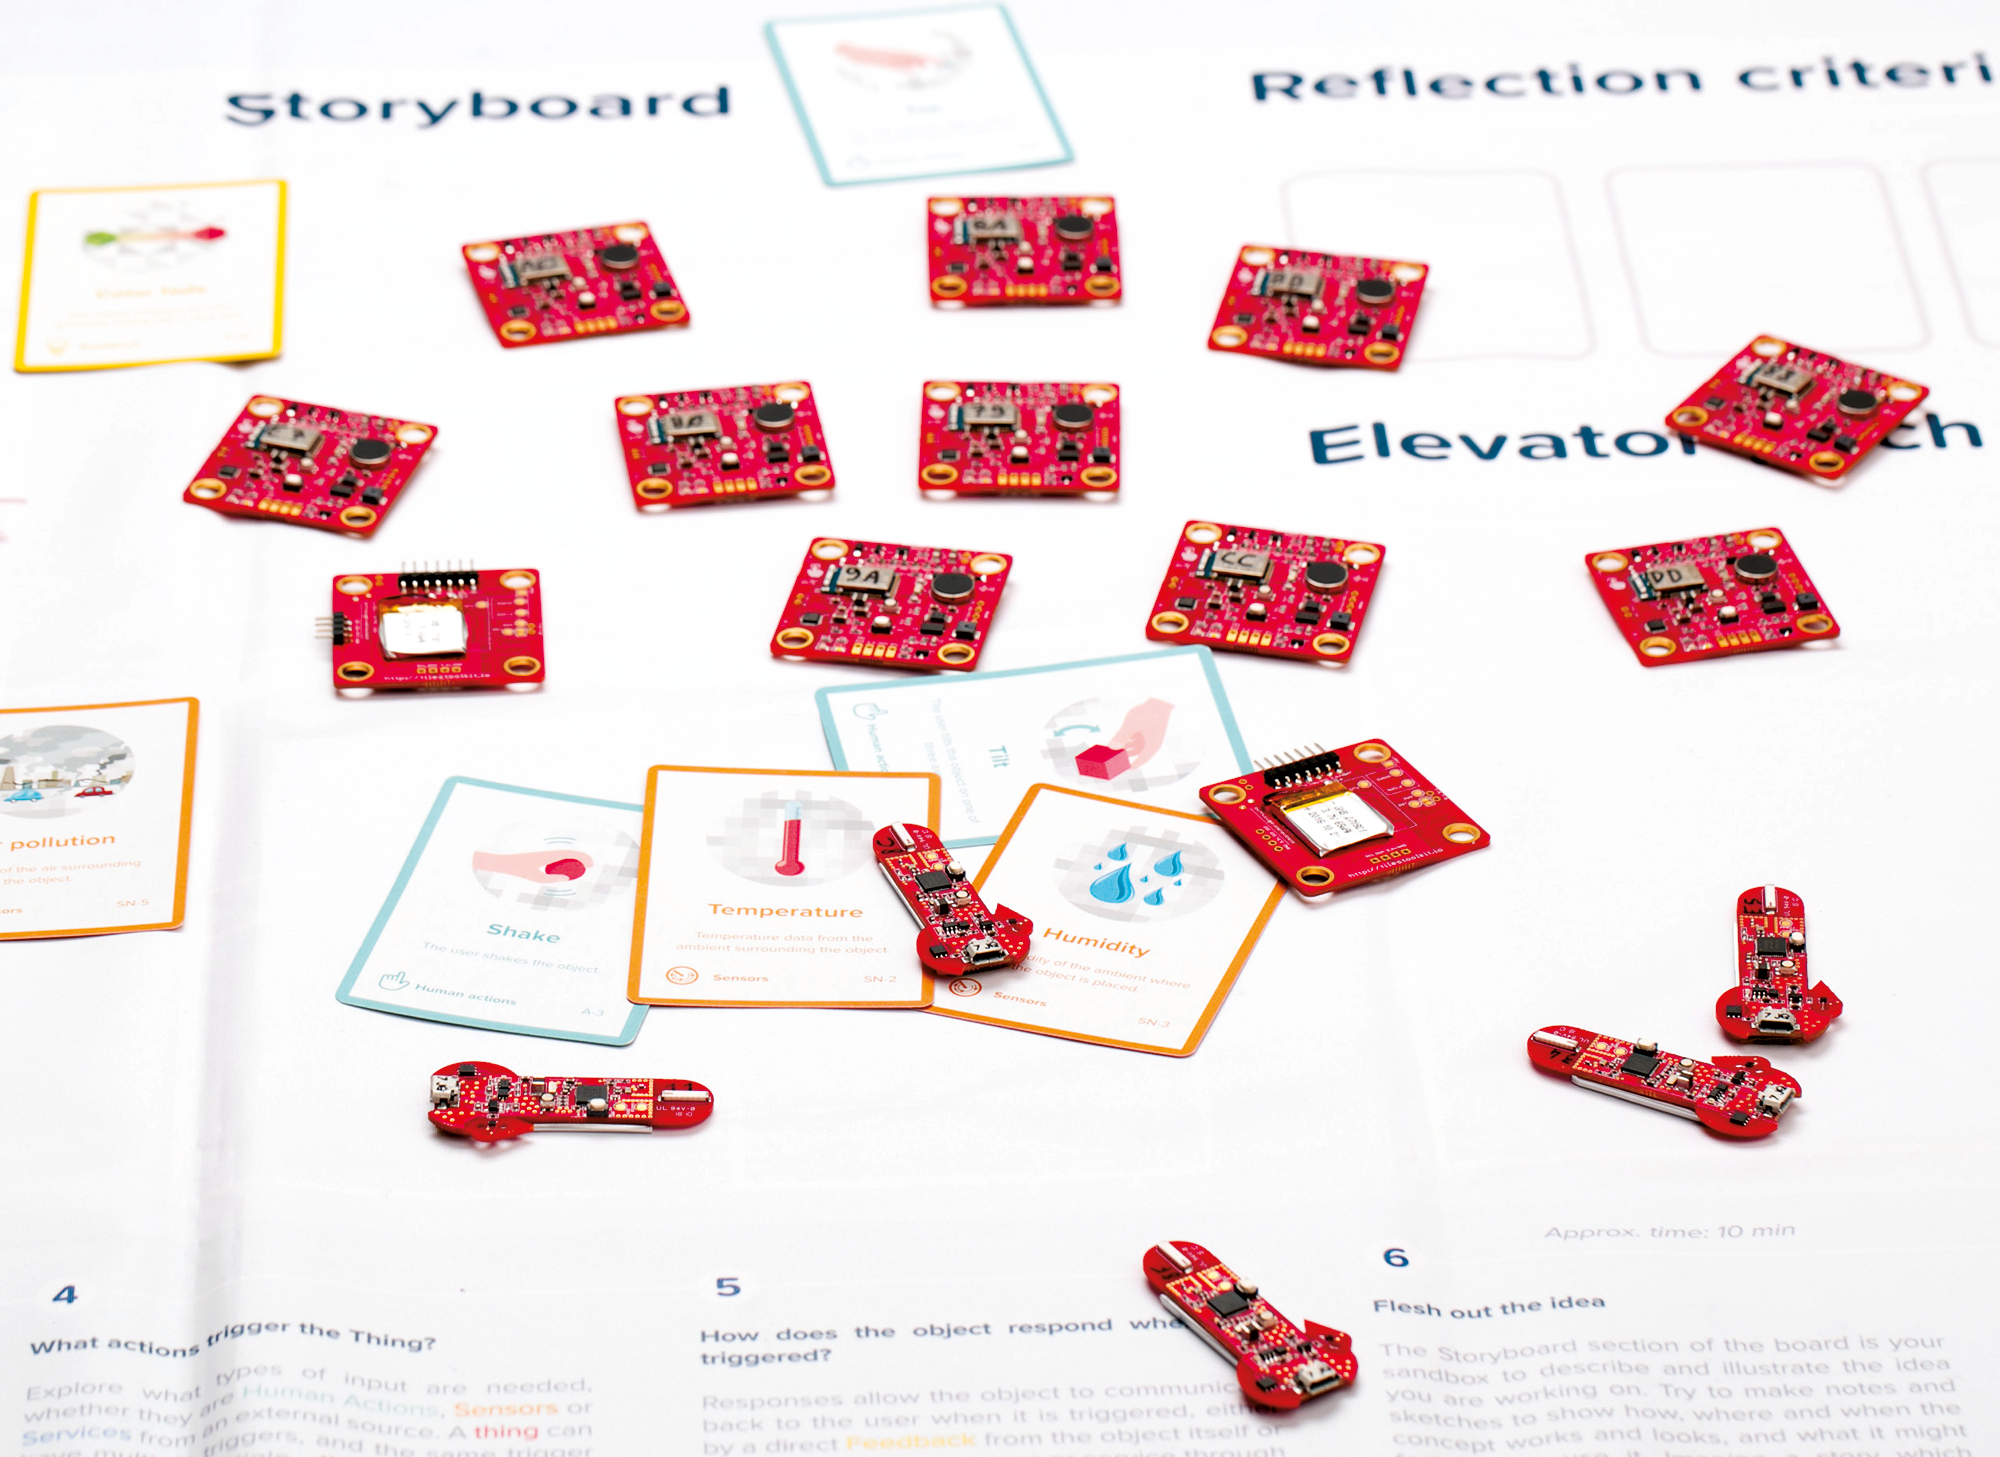
\includegraphics[width=\textwidth]{stickers}
	\caption{Electronic \textit{stickers} employed by the users to prototype the smart objects.}
	\label{fig:stickers}
\end{figure}


\subsubsection{Software Components}

In terms of software, we distinguish two loosely coupled sub-domains: (i) the integrated development environment (IDE) that allows the users to program the application logic and (ii) the platform software stack running on the \textit{stickers}, the cloud and eventually the gateway.

\textbf{\textit{Development Environment}}. The development environment is a cloud-based ambient where the users can program the IoT application logic. The editor used to write the code runs in a browser, sparing the users the installation of any toolchain, driver or software on their personal devices. The programming paradigm employed is a simplified domain-specific language (DSL) based on JavaScript.

\textbf{\textit{Stickers Platform Software Stack}}. The software running on the microcontroller contained in the \textit{stickers} is tasked to fetch data from the sensors attached, command the actuators and expose an API on the network interface. Through the API, the \textit{stickers} can be remotely controlled and can also notify the cloud if new sensor data are available or if any user interaction occurs.

\textbf{\textit{Cloud Platform Software Stack}}. The cloud software acts as a network hub for the \textit{stickers}, exposing their functionalities to the development environment. The development environment, accessible from the browser, is also hosted on the cloud. The cloud IDE is the only interface for the user to program the application logic. To start coding, the user is not required at all to connect any cable or install any software.

\textbf{\textit{Gateway Platform Software Stack}}. The gateway is a device whose main role is to bridge the connectivity between the \textit{stickers} and the cloud. For example, it can provide Bluetooth connectivity to the \textit{stickers} on one side and cellular connectivity on the other, allowing the \textit{stickers} to send and receive events to and from the cloud. We used a smartphone to act as a gateway, and a multi-platform mobile app was developed to handle the connectivity towards the cloud and the \textit{stickers}.

Using IP-based wireless connectivity on the \textit{stickers}, it is possible to reduce the complexity of the gateway, since it would simply need to forward the IP packets between the network interfaces. This way, the gateway would work at a lower level of the ISO/OSI network stack, thus requiring fewer computational resources compared to a routing task involving the full translation of application-level protocols. The use of a gateway can possibly be omitted altogether using new low-power microcontrollers with embedded cellular connectivity. Thanks to these solutions, the \textit{stickers} can have direct access to the cloud like a smartphone.


\section{Integration of the Toolkits in Prototyping}

With the Tiles ideation toolkit and the RapIoT toolkit, we introduced a path of continuity between the phases of \textit{problem definition}, \textit{idea generation} and \textit{design} and the creation of a prototype for quick and tangible exploration of creative ideas.

Connecting these two stages, without limiting the outcome to a simple idea, means supporting the users in the conceptual as well as in the practical stage. This continuum is important for several reasons, as explained by Brown \autocite*{brown_strategy_2005}:

\begin{itemize}
    \item Ideas presented using only words are highly open to interpretation, and require supremely engaging storytelling skills to be relied upon effectively. Words mean different things to different people, especially if they come from different backgrounds.
    \item A prototype, or a demonstrator of the idea, describes a concept in a way that is not open to many interpretations. Physically experiencing the nature of a prototype facilitates convergence towards a shared view.
    \item A prototype is simultaneously an evaluative process (it generates feedback and enables corrections) and a storytelling instrument (it visually describes a strategy or an idea).
\end{itemize}

The goal is not to create a close approximation of the finished product, but to build something that is rough and ready and works, an instrument to elicit feedback, to unlock intuitions from the people \autocite{brown_strategy_2005}.

The Tiles IoT framework guides the users through the different phases in a consistent way. The theoretical concepts, the building blocks of the toolkits and the abstractions employed are introduced gradually and progressively enriched during each phase. This steady learning curve allows capitalising the efforts towards the prototype, avoiding drastic shifts of paradigm or introducing gaps in the knowledge required, which might hinder the creative process.


\section{Lowering the Bar: Non-Experts as Target Users}

The Tiles ideation toolkit and the RapIoT toolkit were designed to keep the entry barriers low, at the same time allowing the users to generate an idea, illustrate it and create a prototype during workshops lasting less than a day.
The target group is represented by \textit{non-expert} users, described in Section~\ref{sec:non-experts}, who have some proficiency in the basic paradigms used by high-level programming languages such as JavaScript abd Python. Upper secondary school students often belong to this category.

The holistic approach of the Tiles IoT framework allows non-experts to actively contribute during tasks that have traditionally required specific technical skills, like low-level programming, assembly and prototyping of electronics for augmented objects.

Since the RapIoT toolkit targets low-complexity applications and non-expert users, it might be beneficial to employ a programming abstraction that requires a lower level of programming skills than the ones usually required by textual programming languages. Visual programming languages like Scratch\footnote{https://scratch.mit.edu/} or Node-RED\footnote{https://nodered.org/} have been successfully employed in rapid prototyping, and their steep learning curve is appreciated by novices \autocite{booth_end-user_2013}. These well-established programming paradigms are easy to use and are understandable interfaces for the configuration of IoT devices \autocite{houben_physikit_2016}.


\section{Identified Values of the Toolkits}

Here, the generic values of the toolkits, identified by Ledo et al. \autocite*{ledo_evaluation_2018} and reported in Chapter~\ref{cha:toolkits}, are recalled and contextualised for the toolkits described in this chapter.

\begin{itemize}
    \item \textbf{G1}: Reducing the Authoring Time and Complexity. The toolkits presented are designed to be used during activities lasting less than a day. Complexity is kept under control by gradually introducing new concepts along the process.
    \item \textbf{G2}: Creating Paths of Least Resistance. The defined rulesets and pathways are present in the toolkits in the form of step-by-step instructions on the playbook and through constraints guiding the coding and prototyping activities.
    \item \textbf{G3}: Empowering New Audiences. The target group of non-expert users, defined as in Section~\ref{sec:non-experts}, are fully involved in the authoring process and represent audiences not traditionally addressed by IoT toolkits.
    \item \textbf{G4}. Integrating with Current Practices. The use of cards and other building blocks that are already familiar to many users facilitates development and integration.
    \item \textbf{G5}. Enabling Replication and Creative Exploration. Ideation, prototyping and replication of creative ideas are used to explore new concepts and tools.
\end{itemize}


\section{Learning from the Past: Tackling Current IoT Challenges}

We are all familiar with what the World Wide Web is and how it works. It is nowadays an essential part of our daily routine, work and leisure. However, we cannot say the same about IoT, despite it being a concept as old as the web. In order to provide the reader with a provocative perspective of the IoT field in its current status, in the following, I will describe the web as if it shares the shortcomings and limitations of the current IoT technologies.

\begin{framed}
Alice just bought a new computer, produced by \textit{BigTechCompany}. She also bought from the same company a cable modem, which will allow her new computer to connect to the telephone line and access the Internet. Using the browser that she found pre-installed on her computer, she quickly discovered that she can only access a limited number of websites, which are associated with or supported by \textit{BigTechCompany}. In order to visit some of the other websites, she needs to install a second browser on her computer, but the website selection will still be quite limited. She wonders how she can connect to the websites associated with \textit{SmallTechCompany}. It seems that a few of the websites of \textit{SmallTechCompany} can be accessed by replacing her cable modem with one produced by \textit{SmallTechCompany}. However, to access all of the websites of \textit{SmallTechCompany}, there is no other way than buying a new computer produced by \textit{SmallTechCompany} itself, which is also the only computer able to run the browser issued by the company.
She decides to buy the required hardware, even if it looks like a waste of money given that she already has a brand-new computer. After a few months, to her great disappointment, \textit{SmallTechCompany} goes out of business, leaving Alice with an expensive computer-shaped paperweight: the websites of \textit{SmallTechCompany} are taken offline, the browser cannot access any other content and the modem does not even connect anymore to the Internet. Alice hopes for someone to take over the work of \textit{SmallTechCompany}, but she gets to know that \textit{SmallTechCompany} did not release any documentation or specification covering the technologies used. That knowledge was condemned to disappear with the company.
\end{framed}

It is difficult to imagine how this fictional scenario could support widespread adoption, growth, accessibility and security. For example, adoption is inhibited by proprietary specifications, accessible only by payment. Growth and accessibility are limited if only a few market players have the resources to develop the technology. Security is affected since it will not be guaranteed if the company licensing the technology goes out of business, leaving the devices of the users exposed \textit{in the wild}.

Many researchers and IoT experts have precisely identified these issues and proposed solutions that build on the aspects that made the web so popular and so different from what described above. This approach was adopted by Guinard and Trifa \autocite*{guinard_building_2016} and was described in their \textit{web of things} architecture. They advocated that the simplicity and openness of the web and its standards are likely what enabled the web we know today. The lingua franca of the web enabled the users to access any webpage without installing anything and has been a major factor in its success. By enabling webpages, browsers, servers and services to all speak the same application language, the integration of a large variety of content was incredibly simplified. Unfortunately, no equivalent enabler has yet been found for devices and applications in IoT \autocite[p. 23]{guinard_building_2016}.

Their pioneering work was not limited to a theoretical exploration. A W3C working group has been established\footnote{https://www.w3.org/WoT/WG/} and is currently active in drafting an open standard based on the \textit{web of things} model. A preliminary implementation of the standard is already in use by the Mozilla IoT gateway\footnote{https://iot.mozilla.org/}, an open-source hub for home automation.

Many other standards, protocols and data models are available in the IoT world. To cite a few examples, the Bluetooth GATT profiles\footnote{https://www.bluetooth.com/specifications/gatt}, the Open Connectivity Foundation oneIoTa\footnote{https://www.oneiota.org/} and the Zigbee Dotdot\footnote{https://www.speakdotdot.com/} all define a mix of APIs, data models and communication protocols to be used with different \textit{things}. Similar ecosystems have been designed and implemented by Apple, Google and Amazon.
These standards are often not as open and accessible as the web ones, and they fall short when addressing IoT under a user-centred perspective. For example, they define APIs to communicate with objects, to allow data sensing and collection, but none of them have yet addressed human interaction primitives and gestures used to manipulate objects, using structured, open and accessible specifications.


\section{Vision for the Tiles IoT Framework}

With the Tiles project, we experimented with and evaluated a user-centred approach to IoT based on physical objects and tangible interfaces. In order to support the target user group of non-experts, our aim was to simplify the setup and deployment tasks of a typical IoT application, providing an intuitive development environment that allows rapid prototyping and fast exploration of ideas. These goals very well fit with the philosophy of the \textit{web of things}, which in addition enables community work, transparency, openness and accessibility. Building future advancements on top of this model will prevent vendor locks and expensive implementations and will allow the Tiles \textit{stickers} to be employed for multiple use cases and by multiple actors, with minimal integration costs even when detached from the RapIoT platform.

Outreach, education and open collaboration are the main principles driving the work of W3C. The adoption of a model backed by an international standards organisation such as the W3C guarantees a solution that is not tied to the fate of a commercial corporation and is royalty-free to use for anybody.
\chapter{Theoretical Underpinning}
\label{cha:theory}


In this chapter, the predominant theories defining the approach adopted by the Tiles toolkit and the IoT ideation process will be presented. It is worth mentioning that the investigation work that led to the creation and evaluation of the Tiles toolkit and the IoT ideation process was grounded in additional theories such as UCD, end-user development (EUD), SCL and CSRL and took advantage of the HCI guidelines, for example, in connection to usability. Some of these theoretical domains have been addressed in Chapter~\ref{cha:smart-cities}, whereas others will be covered in Chapter~\ref{cha:research-methodology}.


\section{Co-Design}

In the context of sustainable HCI, distinctions were drawn between seeing the behaviour of the users as the cause of environmental problems and gathering needs and opportunities from users to inform design \autocite{disalvo_mapping_2010}. By means of participation and co-design, people can provide direct input to \textit{solve the problem of the users}, designing thus their own behaviour change \autocite{lockton_designing_2014}.
Through co-design, users build empathy with the solution they contributed to. Co-design allows multiple voices to be heard; it is fair and ethical to involve those whose livelihoods, environments and lives are at stake in the decisions that affect them \autocite{perlgut_community_2005}.
Employing participatory approaches empowers people, allowing shared responsibilities among stakeholders. This can create credibility and trust, emphasise diversity in stakeholder involvement and increase the likelihood that the final product will meet the expectations \autocite{pettersen_ethics_2008}. The role of the researchers is to support, explain, fight and help negotiate design tensions, recommending methods and tools. Controlling the creative process and managing the users are practices that do not belong to the co-design methodology.

Under the umbrella of co-design, various approaches and methods are used, which result in different combinations between the level of involvement of the stakeholders and the number of different stages of the design process covered. Many studies that apply co-design in the smart city context involve the users during the brainstorming and idea generation phase \autocites{mitchell_empirical_2016}{schuurman_smart_2012}{mechant_e--deliberation_2012}{fu_building_2014}, whereas others consider the shareholders only in a tokenistic way, limiting their contribution to the act of providing simple feedback or rating the final solution \autocite{reiersolmoen_delta_2017}.
Although participation is historically emphasised at the moment of idea generation \autocite{cross_design_1971}, modern co-design practices can extend beyond the very first phases of the design process, including the users more deeply throughout the whole process. This is facilitated by the lower entry barriers achievable while using recent technologies to address specific tasks, which have been a prerogative of professionals only a few years ago.

In this thesis, I will describe how co-design practices have been used to drive brainstorming and idea generation and also how co-design can be extended beyond its traditional scope. This aspect characterises how the toolkits described in Chapter~\ref{cha:iot-framework} are intended to be used \textit{in the wild}. The objective is to promote a co-design process where potential stakeholders are brainstorming, designing and prototyping a solution for a problem that affects them.
This opportunity has been explored in few studies, which is demanding given the social and technological challenges that come attached to practices like design validation with the user and collaborative implementation of ideas.


\section{Tangible User Interaction with Smart Objects}

The work described in this thesis embraces the understanding of IoT and ubiquitous computing proposed by Rogers \autocite*{rogers_moving_2006}, which challenges the original calm computing vision of Weiser \autocite*{weiser_computer_1991}. Weiser depicted a scenario where user interaction is anticipated and predicted by a sensing smart environment, relegating the user to a mostly passive role.
This approach led to poor results in research and prototyping on ubiquitous computing and IoT, mainly because trying to predict human will is a difficult artificial intelligence problem \autocite{rogers_moving_2006}. Even small errors are perceived as annoying and frustrating from the user, to the point of dismissing and abandoning the technology in use.

Such vision presents challenges also from a sociological point of view. Users should be encouraged to interact and make critical decisions; the technology can support this process, improving awareness, stimulating reflection and possibly engaging the user in the activity.
This way, it is possible to introduce new techniques to change the attitudes and behaviours of people, on the basis of social learning, for sustainable common objectives.

Rogers did not completely discard the vision of Weiser but rather tried to entertain other possibilities besides calmness for research on ubiquitous computing.
Examples include extending and supporting personal, cognitive and social processes such as habit-changing, problem-solving, creating, analysing, learning or performing a skill \autocite{rogers_moving_2006}.
Rogers advocated that research in the field should be aimed at better understanding human activity rather than trying to predict and intervene in situations that already work reasonably well, with a high risk of unwanted or unpredictable outcomes. This people-oriented perspective was also envisioned by Streitz et al. \autocite*{streitz_designing_2005} in the smart object research domain. They prospected smart objects as empowering artefacts for decision-making, supporting mature and responsible actions.

In order to tackle the challenges described in Section~\ref{sec:motivation}, I chose to adopt an \textit{object augmentation} strategy in order to create TUIs based on smart objects. As described by Kuniavsky \autocite*[p. 254]{kuniavsky_smart_2010}, object augmentation starts from everyday, non-digital objects and augments them with technology, while their purpose and familiar characteristics are maintained.
This family of interfaces, also called sensing-based interfaces, allows for new interaction paradigms that explore the opportunities lying beyond traditional human-computer interfaces such as screens, keyboards and mice \autocite{van_dam_post-wimp_1997}. TUIs are characterised by the embodiment of interaction in physical objects, they emphasise the physicality of interaction through the coupling of physical and digital representations \autocite{markova_tangible_2012}.
TUIs take advantage of the physical skills of the users, exploiting knowledge of the everyday, non-digital objects \autocite{jacob_reality-based_2008}.
These physical interfaces are capable of delivering relevant information at appropriate times, which is critical for triggering learning and sustaining reflection \autocite{rogers_framework_2006}. In addition, they can be embedded into the environment and represent data streams in a physical way \autocite{hornecker_getting_2006}. User interaction then moves \textit{off the screen}, becomes more natural and can be distributed in space \autocite{dourish_where_2004}.

\begin{figure}[hbt]
    \centering 
	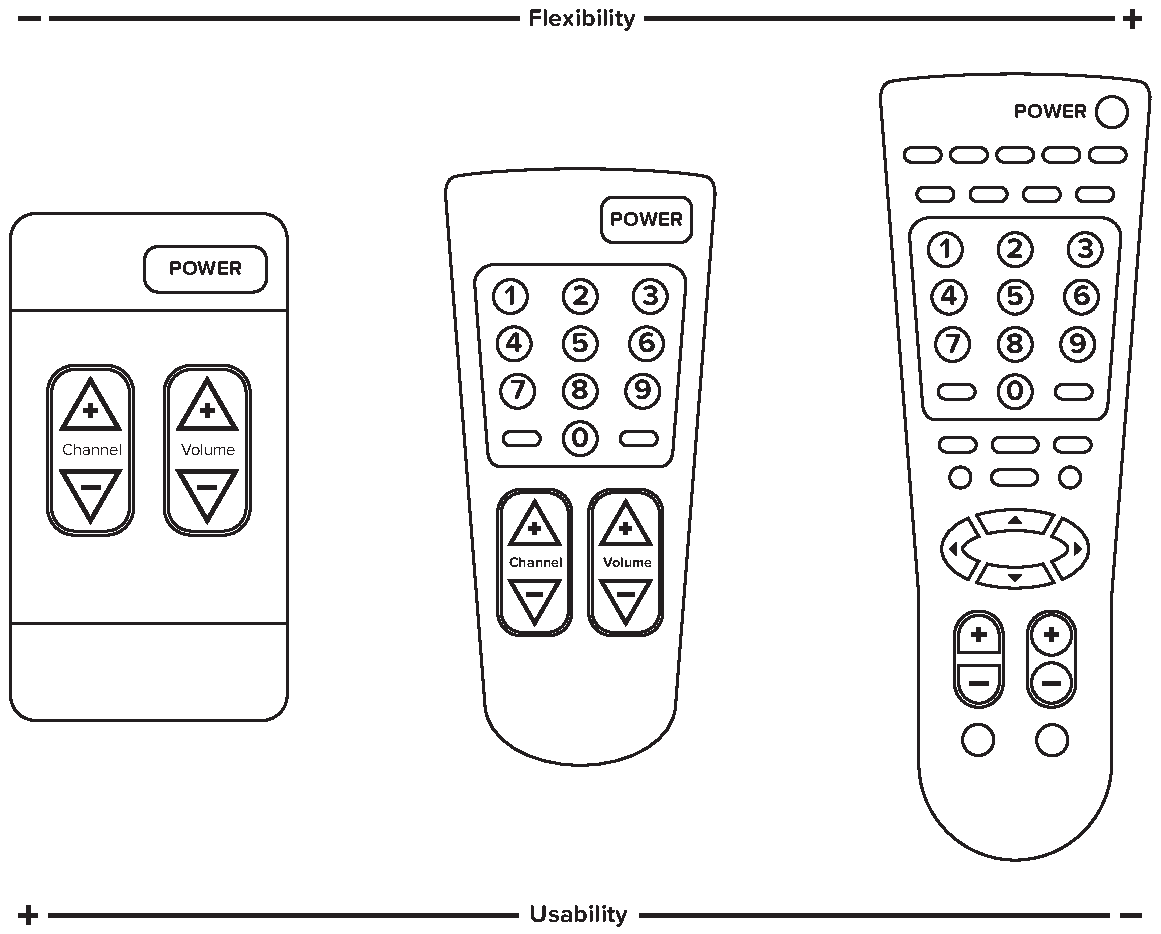
\includegraphics[width=\textwidth]{remotes}
	\caption{A visual example of how a simple design can be easy to use, whereas a more flexible and feature-rich one is less usable \autocite[p. 103]{lidwell_universal_2010}.}
	\label{fig:remotes}
\end{figure}

Advocating the well-known design maxim \textit{\enquote{jack of all trades, master of none}}, Lindwell et al. \autocite*[p. 102]{lidwell_universal_2010} presented the trade-off between \textit{flexibility} and \textit{usability} in design: flexible designs can perform more functions than specialised ones do, but they perform these functions less efficiently (Fig.~\ref{fig:remotes}). Jacob \autocite*{jacob_reality-based_2008} transferred this concept to TUIs, proposing a trade-off between \textit{reality} and \textit{versatility}. TUIs are specialised by their physical affordances and constraints and, thus, can perform a limited set of tasks with a high level of realism or simplicity. Moreover, TUIs foster collaboration \autocite{rogers_configuring_2003}, in which they increase the visibility of the actions of others and allow for concurrent interactions. TUIs extend the static representation of an object with an intangible, dynamic one. TUIs were part of the original vision of Weiser and have been then researched by Rogers as well as Ullmer and Ishii \autocite*{ullmer_emerging_2000}, among others.



\chapter{Research Methodology}
\label{cha:research-methodology}

The aim of this chapter is to present the research methodology adopted during the work described in this thesis. Not all the methods have been explicitly elaborated in the papers included in Part II, but they have been nevertheless important while framing the studies and designing the tools employed during my research.


\section{Research Philosophy}

The leading research philosophy adopted was \textit{phenomenology}, a variation of \textit{interpretivism}. According to the interpretivist approach, it is important for the researcher as a social actor to appreciate differences between people \autocite{saunders_research_2009}. Studies adopting the interpretivism research philosophy usually focus on meaning and may employ multiple methods in order to reflect different aspects of the issue. During my research, quantitative data were collected and used to validate theories and outcomes; however, we could not refrain from considering subjective human interests and meanings to validate the results.

The \textit{phenomenology} branch describes the philosophical approach asserting that what is directly perceived and felt is considered more reliable than explanations or interpretations in communication \autocite{remenyi_doing_1998}. Ideas and theories are generated from a rich amount of data mainly by means of induction, whereas stakeholder perspective may have its reflection on the study.


\section{Design as Research}

The topics proposed in Chapter~\ref{cha:introduction} have been researched using design science research and researching design methods \autocite{hevner_design_2010}.
Design as Research encompasses the idea that performing innovative design that results in clear contributions to the knowledge base constitutes research \autocite{hevner_design_2010}. Knowledge generated via design can take several forms, including constructs, models, methods and instances \autocite{march_design_1995}.
Design as Research thus provides an important strand of research that values research outcomes that focus on the improvement of an artefact in a specific domain as the primary research concern, and then it seeks a broader, more general understanding of theories and phenomena surrounding the artefact as an extended outcome \autocite{hevner_design_2010}.
A key insight into how to perform design science research can be gained by understanding the existence of three design science research cycles in any design research project, summarised in Fig.~\ref{fig:design-cycles} and further detailed by Hevner and Chatterjee \autocite*{hevner_three_2007}.

\begin{figure}[ptb]
    \centering 
	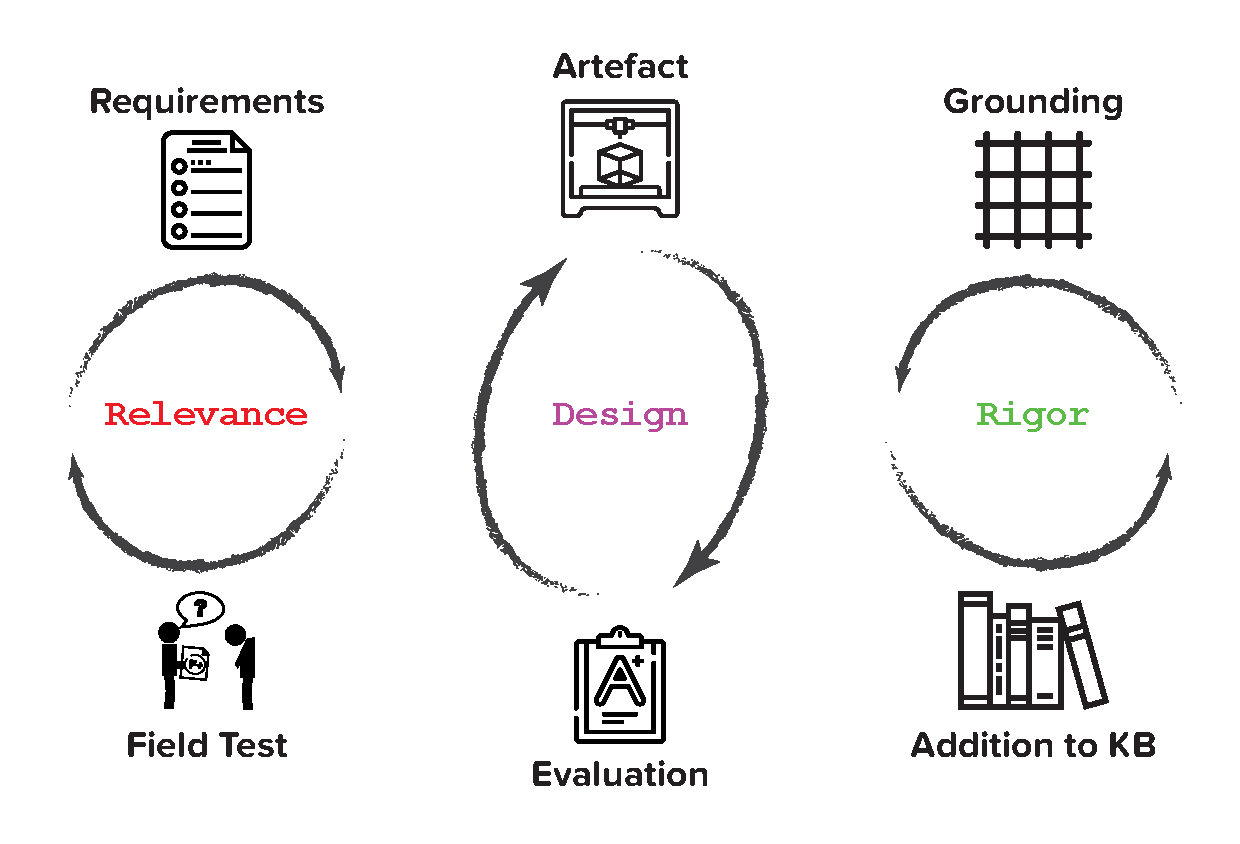
\includegraphics[width=\textwidth]{design}
	\caption{Schema of the three design science research cycles, based on Hevner's model \autocite*{hevner_three_2007}.}
	\label{fig:design-cycles}
\end{figure}


\subsection{Relevance Cycle}
The relevance cycle initiates design science research with an application context that not only provides the requirements for the research (e.g. the opportunity/problem to be addressed) as inputs but also defines the acceptance criteria for the ultimate evaluation of the research results \autocite{hevner_design_2010}.
This process connects design science research with the application context. The iteration allows for improvements and refinements of the requirements and for validating incremental results using field testing feedback.

During my work, a user-centred approach characterised the work pertaining to this cycle. Data collected during user studies contributed to the process of constant refinement and improvement of the tools and technologies designed.

\subsection{Rigor Cycle}
The rigor cycle ensures that research is grounded in relevant literature and has solid foundations. This includes considering the state of the art, past knowledge is in fact essential to drive and support innovative research.

A literature mapping on topics relevant to my research was conducted as part of this cycle. This represented the starting point, building a solid knowledge foundation and theoretical background for subsequent research.
Design science research can also contribute to improving the state of the art and the knowledge base. This way, the rigor cycle loop is then closed, providing a tangible contribution to the field of research.

\subsection{Design Cycle}
The internal design cycle is the heart of any design science research project. This cycle of research activities iterates more rapidly among the construction of an artefact, its evaluation and the subsequent feedback to refine the design further \autocite{hevner_design_2010}.
It is important to note the difference between the design cycle and the relevance cycle. The first iterates and validates the artefact against the requirements, whereas during the second the objects of the iteration and refinement are the requirements themselves, not the artefact.
The design cycle should be well balanced between the building and evaluation processes. Scarce commitment in one of the two phases will lead to poor overall results.
The design cycle is quite independent of the relevance and rigor cycles, and it is also executed more.


\section{Research Strategy and Methodological Choice}

In order to implement the main research strategy, several methods have been adopted. A mix of qualitative and quantitative research methods have been used to account for the unpredictability in field studies \autocite{rogers_why_2007}. Mixed methods research fit well with the research objectives because of its potential with respect to understanding and explaining complex organisational and social phenomena \autocites{cao_interactions_2006}{mingers_combining_2001}.
Further, mixed methods research has received much attention in the social and behavioural sciences recently (for a review, see \cite{tashakkori_mixed_2008}).
During my research inquiry, observations, notes and video and audio recordings were the primary means used to collect data during the field studies with the users (Fig.~\ref{fig:user-study}). Pre-post questionnaires, interviews, quiz games and focus groups were usually employed to evaluate the artefacts employed and the process adopted and to assess the perceived outcome of the user experience.

\begin{figure}[ptb]
    \centering 
	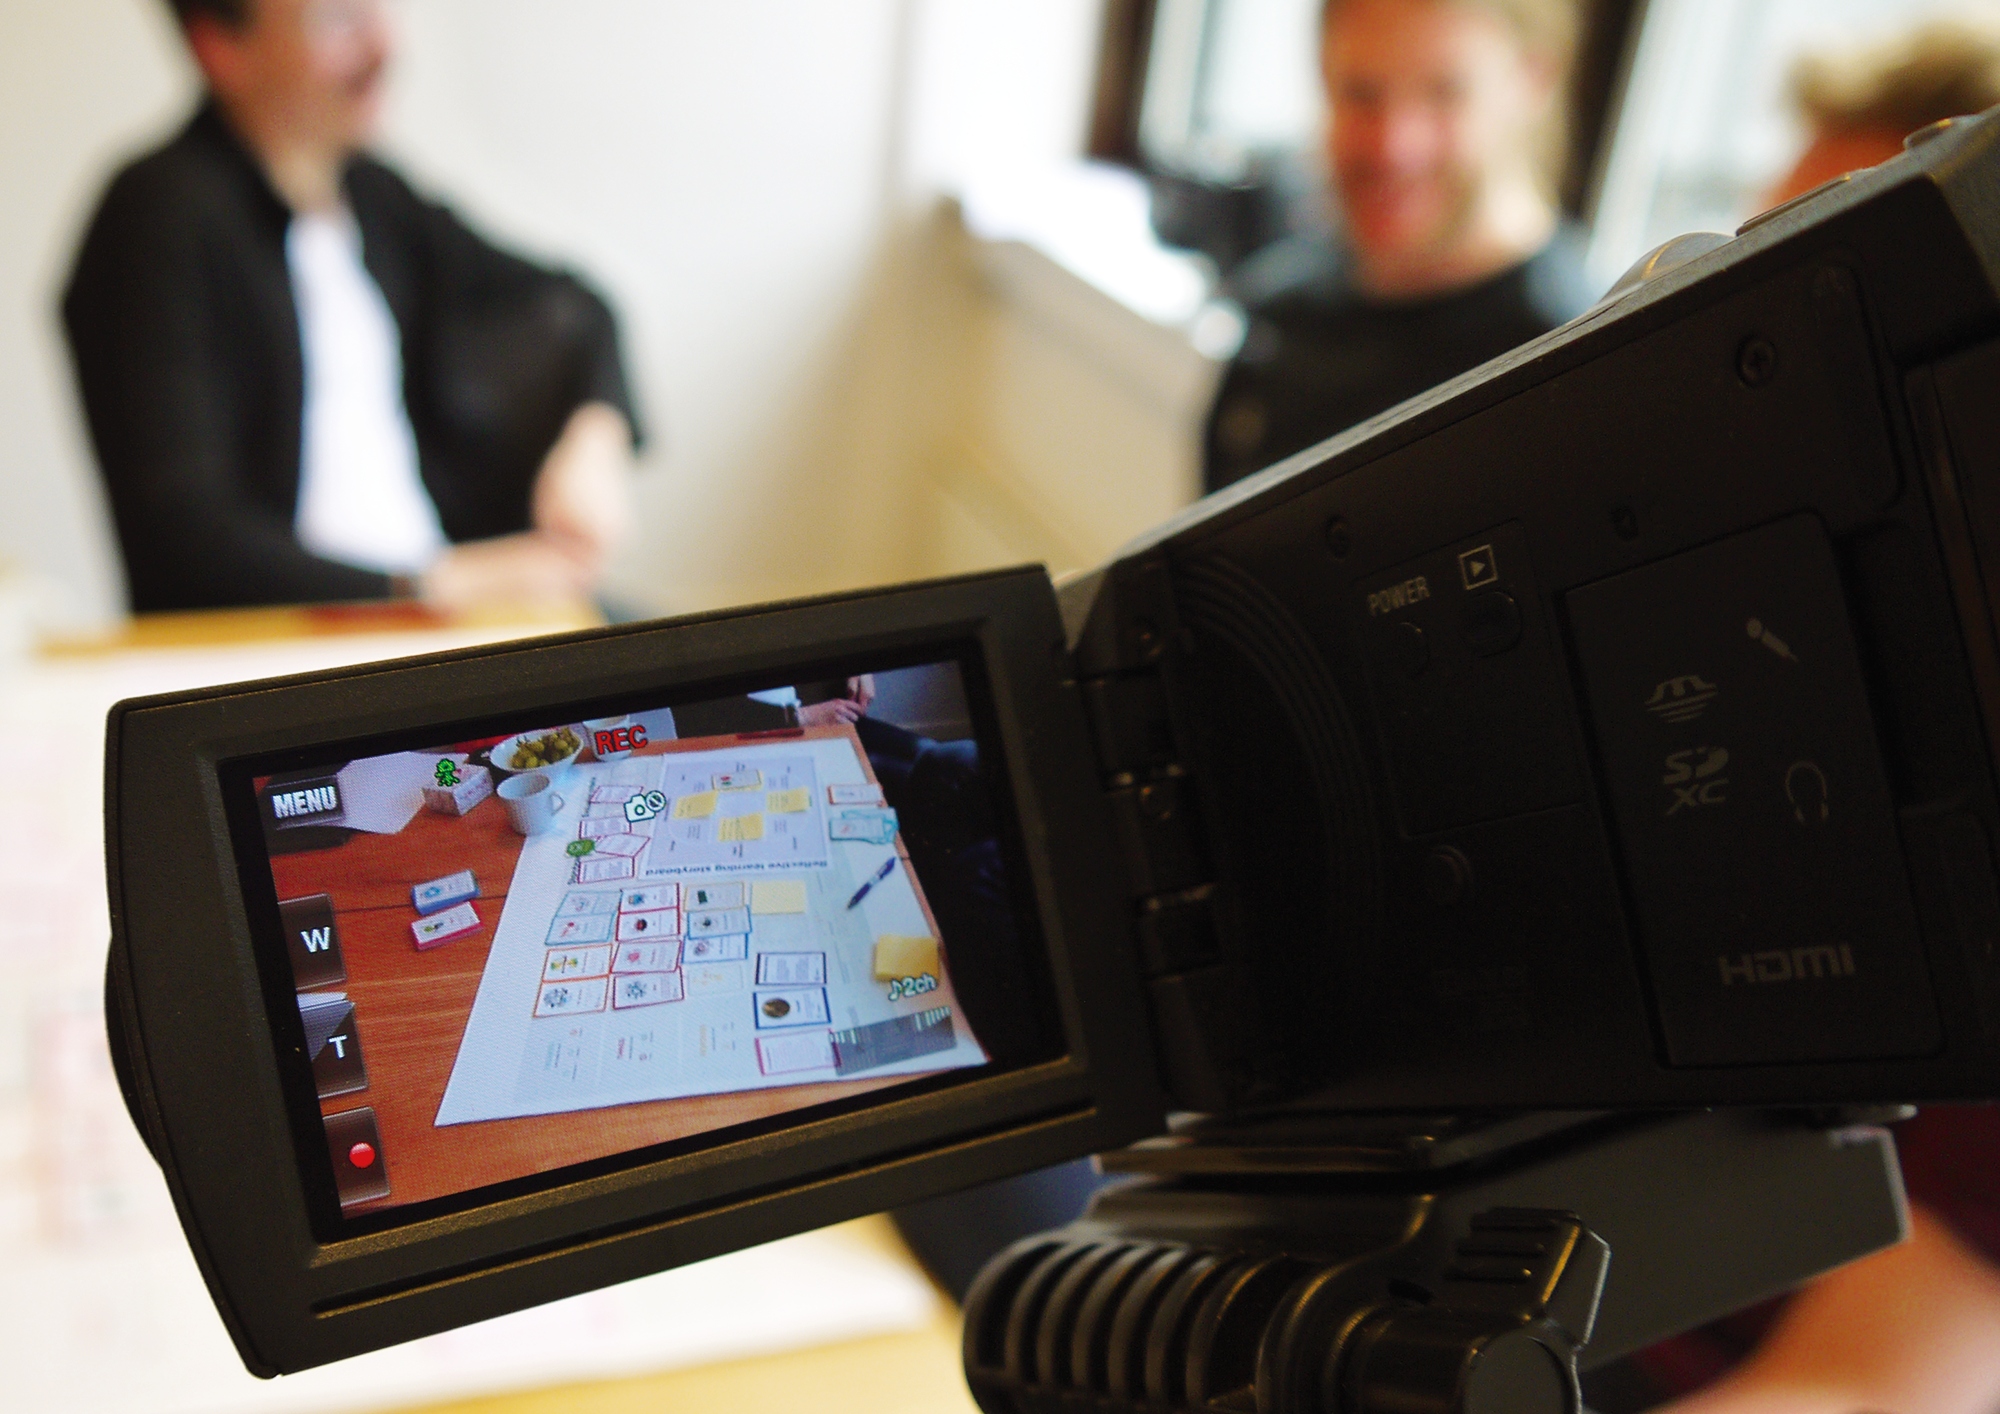
\includegraphics[width=\textwidth]{camera}
	\caption{Video recording of the user interaction occurring around the Tiles cards and cardboard. The brainstorming workshop pictured was one of the studies included in P4.}
	\label{fig:user-study}
\end{figure}


\section{Research Activities}

During the progress of my research, different activities and outcomes contributed to the three cycles of the \enquote{Design as Research} methodology: \emph{relevance}, \emph{design} and \emph{rigor} cycles.

As a first step, I performed a literature mapping of the technological applications in smart cities (P1). The identified needs, challenges and research opportunities were used to drive and support the following steps.
Early design ideas were turned into exploratory low-fidelity prototypes and tested on the field with the users.
Subsequent iterations both improved and specialised the prototypes, building on the experience matured during the field studies and the domain knowledge acquired while mapping the literature.

The central course of my research concentrated on the user evaluation of different prototypes targeting the \textit{idea generation} and \textit{design} phases of the Tiles IoT framework process. Other activities involved the design, creation and evaluation of technological tools connecting and extending the \textit{design} phase into \textit{rapid prototyping}. Fewer iterations were performed on such tools because of the increased complexity of the manufacturing process. However, valuable insights, prototypes, design recommendations and knowledge resulted as an outcome. Working prototypes were also used to validate and extend theories as part of the \emph{rigor cycle}.
Research outcomes were reported in academic publications (Chapter~\ref{cha:results}) and research contributions (Chapter~\ref{cha:contributions}) emerged. Throughout the process, the literature on co-design and tangible interaction (Chapter~\ref{cha:theory}) informed the design work.

\subsection{User Studies}
\label{sec:user-studies}

The primary investigation method selected to understand the domain, familiarise with the target users and evaluate the artefacts produced during the design cycle was \emph{design workshops} (Fig.~\ref{fig:workshop}). These workshops were used both to validate the tools employed and to inform the next design iteration. Insights pertaining to possible improvements or defects were gained from direct experience in the field and extracted from the data collected during the workshops.

\begin{figure}[ptb]
    \centering 
	\includegraphics[width=\textwidth]{workshop}
	\caption{A design workshop with university students, part of the studies included in P3.}
	\label{fig:workshop}
\end{figure}

The typical setting for the majority of the studies was a design workshop where participants worked in groups of two to six people. The objective for most of the workshops was to generate a design idea for an IoT application, adapted to solving a particular problem for a specific end-user. The IoT application idea included the use of smart objects designed by the participants during the workshop. During some of the workshops, the participants continued after this initial idea generation phase, physically building the smart objects embedding sensors and actuators. These smart objects were then programmed by the participants to expose high-level functions to the end-users.

The workshop participants were usually students from secondary school up to university level, aged between 13 and 27. Several workshops were also conducted with other categories of users, including researchers, IT professionals, urban planners, teachers and municipality employees. More than 25 workshops were run between August 2016 and April 2018, with more than 500 participants involved.

Observations, researcher notes and questionnaires were the primary means to collect data. In addition, video recordings, interviews and pictures of the produced artefacts were collected during some of the workshops. My role during the workshops was to present the activities and introduce the concepts of IoT and augmented objects. Later on, during the creative phase, my main task was to observe the work of the group, without intervening. The participants occasionally asked for clarifications or support, in which case I was available to provide the required help.

Data captured was handled in observance of the Norwegian University of Science and Technology (NTNU) policies. Occasionally younger users received a gift card after participating. In some workshops, the prize was awarded only to the best ideas generated, voted by the participants themselves.

Data collected was analysed with mixed research methods \autocite{venkatesh_bridging_2013}. The focus of the analysis was twofold. At first, it allowed validating the perceived usefulness, acceptance and learning outcome of the tools used. The outcome of the data analysis also validated the modifications made to the tools, closing the \emph{design cycle}.
The second purpose of the analysis was to spot any usability issue, either in the tools or in the process adopted. Such issues might include confusing guidelines, inappropriate terminology or unclear purpose of the tools at use. These outcomes fed the subsequent iteration of the \emph{design cycle}.

\subsection{Design Iterations}
\label{sec:prototypes}

The work on design and prototyping was driven by the theories adopted and the requirements refined during the user studies. The design process followed a UCD approach \autocites{maguire_methods_2001}{gulliksen_key_2003}. A total of eight prototype iterations were completed. Table~\ref{tab:prototypes} shows an overview of the prototypes created and the technologies used during development in relation to the papers that describe the work.

In order to support the idea generation and prototyping journey, several tools were developed during the Tiles project:

\begin{enumerate}
    \item Several decks of cards, a tabletop cardboard to scaffold the use of the cards and a workshop protocol to guide the process, supporting the problem definition, brainstorming and design phases.
    \item A cloud-based software back-end and development environment to programme the IoT application logic.
    \item Two Bluetooth electronic devices embedding sensors and actuators, supporting rapid prototyping for IoT through object augmentation.
    \item A multi-platform mobile app to facilitate the deployment of the prototypes, serving as a gateway connecting the Bluetooth devices to the cloud software platform.
\end{enumerate}

I contributed to different levels in the design, formalisation of the process, development and scientific evaluation of the components described above, in collaboration with other students and researchers involved in the Tiles project.

\begin{table}
	[!p] \centering \caption{List of prototypes built} \label{tab:prototypes} 
	\begin{threeparttable}
		\begin{tabular}{@{}llllllll@{}} 
			\toprule 
			& & & & \multicolumn{3}{l}{Development}  \\
			\cline{5-7} \noalign{\smallskip} 
			\specialcell[b]{ID\\Ver.} & Name & Released & Prototyping tools & 
			\begin{turn}
				{90}Software
			\end{turn}
			& 
			\begin{turn}
				{90}Hardware
			\end{turn}
			& 
			\begin{turn}
				{90}Material
			\end{turn}
			& Papers \\
			\midrule \noalign{\smallskip} 
			D1 & Tiles & Aug-16 & Personas, Scenarios & & & \textbullet & P2 \\
			D2 & Tiles SC & Jan-17 & Cards, Cardboard & & & \textbullet & P3, P5 \\
			D3 & Tiles Ref & May-17 & Storyboard, Personas & & & \textbullet & P4 \\
			\hline \noalign{\smallskip} 
			W1 & RapIoT App & Jun-17 & Android/iOS framework & \textbullet & & & P6 \\
			W2 & Tiles Temp v1 & Feb-18 & Arduino, Electronics & \textbullet & \textbullet & & Internal \\
			W3 & Tiles Temp v2 & Mar-18 & Electronics & & \textbullet & & P7 \\
			W4 & RapIoT Cloud & Apr-18 & Javascript Node.js & \textbullet & & & P7 \\
			W5 & Tiles Square & Apr-18 & Arduino Firmware & \textbullet & & & P7 \\
			\bottomrule 
		\end{tabular}
		\begin{tablenotes}
			\item
			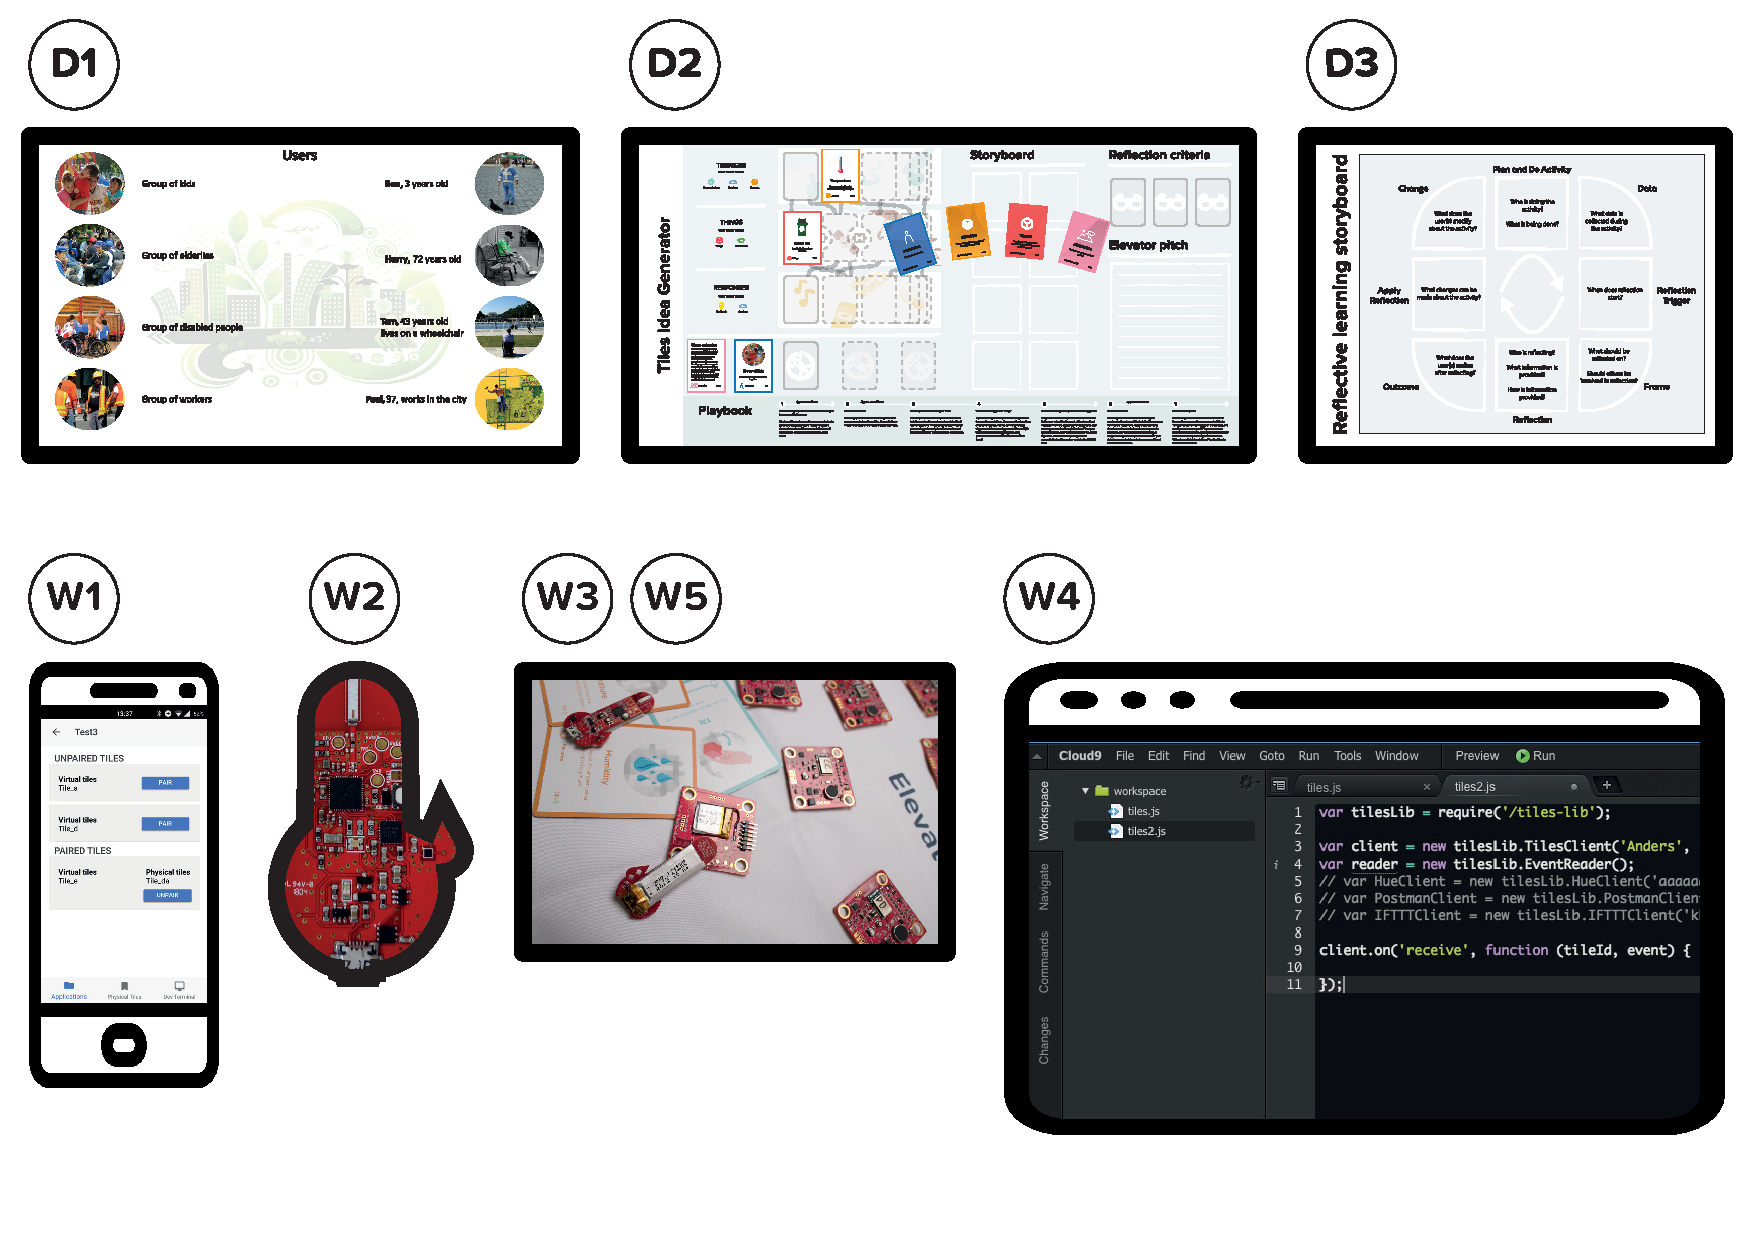
\includegraphics[width=\linewidth]{proto}
		\end{tablenotes}
	\end{threeparttable}
\end{table}

Building the prototypes involved a mix of design, software, hardware and material development. Software was written to create the cloud-based development environment and back-end, the mobile application, and to programme the microcontroller embedded in the electronic devices. The hardware development included the design, manufacturing and testing of electronic boards with embedded sensors and actuators (Fig.~\ref{fig:pcb}). The cards and the tabletop board were designed using desktop publishing and vector graphic editor software. The cards were printed on standard paper, on cardboard and finally on professional-grade playing-card material. The tabletop board was printed on paper, cardboard and various textile materials.

\begin{figure}[ptb]
    \centering 
	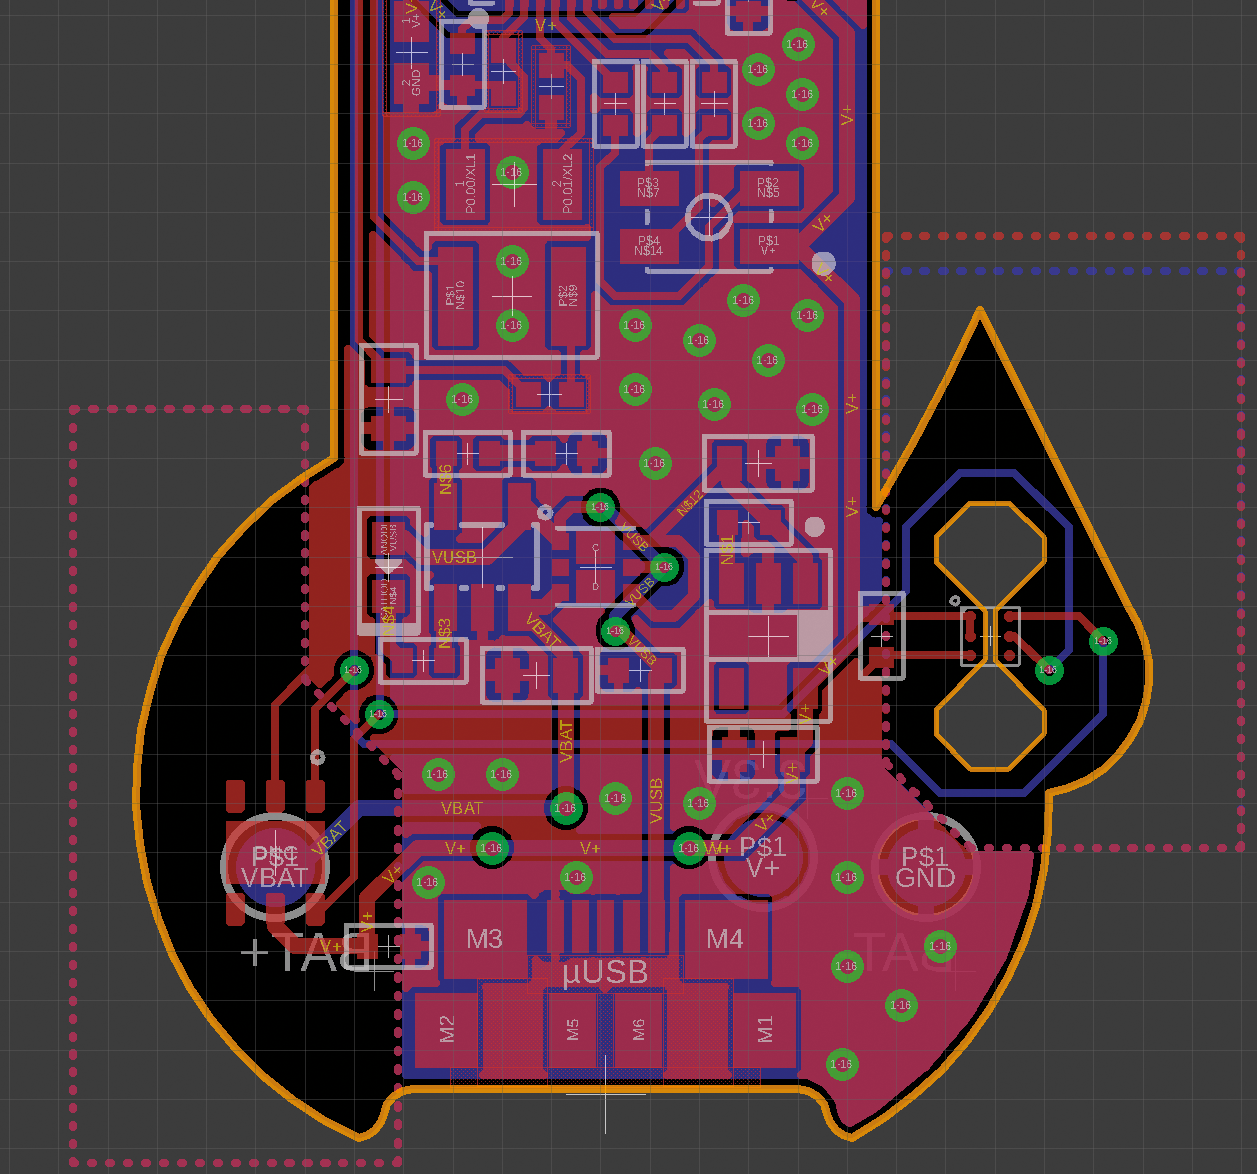
\includegraphics[width=0.7\textwidth]{pcb}
	\caption{Details of the CAD circuit board of the Tiles Temp v2. The temperature and humidity sensors are located in the two dashed areas.}
	\label{fig:pcb}
\end{figure}

Design iterations were usually quick. As soon as incremental improvements and feedback were gathered, a new prototype was produced and tested on the field. Some of the software tools employed included Arduino\footnote{https://arduino.cc} for microcontroller development, the Adobe Creative Cloud suite to design the cards and the cardboard and the Ionic framework to create the mobile application.
Traditional and rapid prototyping approaches complemented the work. The electronics were designed in-house using the Eagle CAD software and built by an external electronics manufacturing company. An external company also printed the cards and the tabletop board in their final version.

After each iteration on the prototypes, an evaluation during a workshop was performed. User testing allowed for maintaining a user-centred design perspective, to introduce new ideas into the process, fix defects and validate the new changes. Some prototypes were built only for internal testing purposes (W2). The Tiles cards, cardboard and workshop process were also part of an expert evaluation in October 2018, where 15 professional designers and IoT researchers from all around Europe provided feedback and suggestions after experimenting with the toolkit during a brainstorming workshop.


\section{User Centred Design Approach}

In order to create more meaningful solutions, which are better tailored to the wishes and needs of the final users, designers have become more concerned about the stakeholders of their creations \autocite{sanders_co-creation_2008}. In the landscape of human-centred design, UCD is one of the approaches that can help in that direction.
UCD and co-design involve value creation in ongoing, productive collaboration with all relevant parties, with end-users playing a central role \autocite{jansen_7_2017}.

Benyon \autocite*{benyon_designing_2014} distinguished four ways in which UCD pays off:
\begin{itemize}
    \item With close user involvement, products are more likely to meet the expectations of the users and their requirements. This leads to increased sales and lower costs incurred by customer services.
    \item System designers tailor products for people in specific contexts and with specific tasks, thereby reducing the chances of situations with a high risk of human error arising. UCD leads to safer products.
    \item Putting designers in close contact with users means a deeper sense of empathy emerges. This is essential in creating ethical designs that respect privacy and quality of life.
    \item By focusing on all users of a product, designers can recognise the diversity of cultures and human values through UCD, a step in the right direction towards creating sustainable businesses.
\end{itemize}

UCD is a design approach that foresees the active involvement of the stakeholders during the design process. Users play the role of \textit{experts of their experience} and participate in knowledge and idea development \autocite{sanders_co-creation_2008}. Research suggests that more innovative solutions can be obtained when co-design techniques are adopted \autocite{trischler_value_2018}, while end-users are believed to have a better perspective of the problem at stake compared to designers, who are not necessarily familiar with the domain addressed as they are with the design methods used to tackle the problem.

Lockton et al. \autocite*{lockton_designing_2014}, advocated the importance of understanding people. Their contexts and social practices of living and working are seen as fundamental to frame problems appropriately, namely, in a way that corresponds to the real lives of the people, instead of basing it on assumptions.
UCD is an iterative process that aims to understand users and their contexts in all stages of design and development. UCD is pertinent to my work especially in connection to the toolkits produced during my PhD and described in Chapter~\ref{cha:iot-framework}. Multiple iterations were performed on the prototypes of the toolkits, addressing usability issues, extending the functionalities and improving the design. These iterations followed a UCD approach: field evaluations, direct user feedback and observations during field work informed each iteration on the design of the toolkit.

\chapter{Results}
\label{cha:results}

This chapter summarises the papers that document the conducted research.


\section{Overview of the Research Papers}
\label{papers}

Research work was published in peer-reviewed journals and conference proceedings. Seven of these publications are included in this thesis; three journal papers and four conference papers. The articles are summarised in this section, including the following:
\begin{itemize}
	\itemsep1pt\parskip0pt\parsep0pt 
	\item Title 
	\item Authors and their roles in the paper 
	\item Abstract of the paper
	\item Publisher 
	\item A short description of how the paper relates to the research questions
\end{itemize}

Papers are reprinted in full in Part II of the thesis.


\section[P1: Technology-Enhanced Smart City Learning: A Systematic Mapping of the Literature.][Paper 1]{Paper 1}
\label{paper-1}

\emph{Title}: Technology-Enhanced Smart City Learning: A Systematic Mapping of the Literature.

\emph{Authors}: Francesco Gianni and Monica Divitini.

\emph{Contributions of the authors}: Gianni led the research and the paper writing. He was actively involved in programming the study and collecting the data. The screening of the papers was performed mainly by Gianni, while articles coding was performed in equal measure by Gianni and Divitini. Divitini also provided general supervision for the research and the paper writing.

\begin{quote}
	\emph{Abstract:} Smart cities are a popular and recognised research topic. In urban spaces, the learning factor is an important component for citizens and local communities. This paper presents a systematic mapping of the literature on smart city learning, with focus on how technology is used to enhance smart city learning. The goal is to map the state of the art and to identify gaps in current research that can prompt new research in this area. Articles were collected from various online databases and relevant journal publications, selected according to defined inclusion/exclusion criteria. Abstracts were coded based on a number of criteria, including e.g. learning goal, used technology, and theoretical approach. Following the coding process results were analysed to identify themes. In the paper we shed light on the current understanding of smart city learning by (i) identifying common scenarios and learning settings; (ii) publication patterns; (iii) technical features in the supporting technology; (iv) learning theories and approaches that are mostly used; and (v) adopted type of research and research methods. The mapping shows that the concept of smart city learning is growing in popularity, with increasing number of publications in this area in the last years. However, the field is rather fragmented, with very different understanding of the concept.  Smart city learning is also emerging as a very complex form of learning, with different stakeholders, learning activities, and technological solutions combined in rich eco-systems. The mapping also points out two largely unexplored areas of technological support, namely the Internet of Things (IoT) and the use of city-related data.
\end{quote}

\emph{Published in}: Interaction Design and Architecture(s) Journal - IxD\&A 27:28--43, (2016).

\emph{Description}: This paper maps the literature in the smart city learning domain. It provides grounding and identifies gaps in the literature, thus supporting the solutions designed in the subsequent works. The findings shed light on a field where modern technologies are seldom employed, and studies do not involve an heterogeneous sample of the citizens, nor they promote active participation.
The paper started the investigation of RQ2, addressing how modern technologies can be tailored to the smart city learning domain.


\section[P2: Tiles: A Card-Based Ideation Toolkit for the Internet of Things.][Paper 2]{Paper 2}
\label{paper-2}

\emph{Title}: Tiles: A Card-Based Ideation Toolkit for the Internet of Things.

\emph{Authors}: Simone Mora, Francesco Gianni and Monica Divitini.

\emph{Contributions of the authors}: Mora created the toolkit and led the paper writing. Gianni created domain specific personas and scenarios used during the evaluation, analysed the data and wrote the second half of the paper. All the authors participated in the data collection during the evaluation workshops. Divitini provided general supervision for the research and the paper writing.

\begin{quote}
	\emph{Abstract:} The Internet of Things (IoT) offers new opportunities to invent technology-augmented things that are more useful, efficient or playful than their ordinary selves, yet only a few tools currently support ideation for the IoT. In this paper we present Tiles Cards, a set of 110 design cards and a workshop technique to involve non-experts in quick idea generation for augmented objects. Our tool aims to support exploring combinations of user interface metaphors, digital services, and physical objects. Then it supports creative thinking through provocative design goals inspired by human values and desires. Finally, it provides critical lenses through which analyse and judge design outcomes. We evaluated our tool in nine ideation workshops with a total of 32 participants. Results show that the tool was useful in informing and guiding idea generation and was perceived as appealing and fun. Drawing on observations and participant feedback, we reflect on the strengths and limitations of this tool.
\end{quote}

\emph{Published in}: Proceedings of the 2017 Conference on Designing Interactive Systems. DIS 2017. 587--598. Edinburgh, United Kingdom: ACM, (2017).

\emph{Description}: This paper introduces the Tiles ideation toolkit, a card based design and ideation toolkit for IoT, see Fig.~\ref{fig:framework} for an overview on how it connects with the Tiles IoT framework. The paper discusses the very first design iteration on the toolkit, its evaluation, strengths and limitations emerged. The Tiles ideation toolkit represents the first step towards improving participation and co-design (Chapter~\ref{cha:theory}) in the smart city learning domain.
The paper investigates RQ1 and RQ2, addressing how non-experts can be included in the development process of technological applications for the smart city domain.


\section[P3: Designing IoT Applications for Smart Cities: Extending the Tiles Ideation Toolkit.][Paper 3]{Paper 3}
\label{paper-3}

\emph{Title}: Designing IoT Applications for Smart Cities: Extending the Tiles Ideation Toolkit.

\emph{Authors}: Francesco Gianni and Monica Divitini.

\emph{Contributions of the authors}: Gianni designed and created the extension of the toolkit, supervised the user study, collected and analysed the data and led the paper writing. Divitini provided general supervision for the design of the extension, research and the paper writing.

\begin{quote}
	\emph{Abstract:} The internet of things (IoT) is gaining momentum as a technical tool and solution for a diverse range of societal challenges. These challenges include smart cities sustainability issues which are widely recognised by decision makers and societies. Despite this, few works try to tackle these challenges empowering citizens through IoT technologies. In this paper we describe how the Tiles toolkit, a card based idea generation toolkit for IoT, has been extended to support non-experts in creating ideas addressing societal challenges that affect modern smart cities. We briefly introduce the Tiles generic toolkit, then we describe in detail the extensions proposed on the cards, cardboard and how the new components are employed in a refined workshop protocol. We report the results obtained during a field study of the extended toolkit, where several groups of students collaborated to generate ideas involving IoT in the smart city. We discuss success and failures, drawing our conclusions after analysing quantitative and qualitative data collected during the workshop. We conclude the article reporting the lessons learned, critical considerations about our experience evaluating the extended toolkit and reflections on possible improvements for future works.
\end{quote}

\emph{Published in}: Interaction Design and Architecture(s) Journal - IxD\&A 35:100--116, (2018).

\emph{Description}: This paper presents the second and final design iteration on the Tiles ideation toolkit. New cards and a new cardboard are introduced, the workshop protocol is refined to improve usability and support for unattended activities without facilitators. Compared to P2, the smart city learning domain is better integrated in the toolkit and in the workshop protocol.
With P3, the research work covering the first three phases of the Tiles IoT framework process (Fig.~\ref{fig:ideation-process}) is considered complete. The artefacts produced and the idea generation process involving non-experts were evaluated, leading to satisfactory results in terms of outcome of creative ideas, learning and support provided. The paper investigates RQ1 and RQ2, addressing how non-experts can generate ideas of IoT applications for smart cities, identifying a specific design strategy centred around tangible interfaces and augmented objects (Chapter~\ref{cha:theory}), and finally linking to the subsequent rapid prototyping phase.


\section[P4: Tiles-Reflection: Designing for Reflective Learning and Change Behaviour in the Smart City.][Paper 4]{Paper 4}
\label{paper-4}

\emph{Title}: Tiles-Reflection: Designing for Reflective Learning and Change Behaviour in the Smart City.

\emph{Authors}: Francesco Gianni, Lisa Klecha and Monica Divitini.

\emph{Contributions of the authors}: Gianni led the paper writing, Klecha designed the study and performed the theoretical grounding. Gianni and Klecha created the extension of the toolkit, participated in the user studies, collected and analysed the data. Gianni performed the last iteration of the study, including the design and production of the artefacts, user study, data collection and analysis. Divitini provided general supervision for the design of the extension, research and the paper writing.

\begin{quote}
	\emph{Abstract:} Modern cities are increasing in geographical size, population and number. While this development ascribes cities an important function, it also entails various challenges. Efficient urban mobility, energy saving, waste reduction and increased citizen participation in public life are some of the pressing challenges recognised by the United Nations. Retaining liveable cities necessitates a change in behaviour in the citizens, promoting sustainability and seeking an increase in the quality of life. Technology possesses the capabilities of mediating behaviour change. A review of existing works highlighted a rather unilateral utilisation of technology, mostly consisting of mobile devices, employment of persuasive strategies for guiding behaviour change, and late end-user involvement in the design of the application, primarily for testing purposes. These findings leave the door open to unexplored research approaches, including opportunities stemming from the Internet of Things, reflective learning as behaviour change strategy, and active involvement of end-users in the design and development process. We present Tiles-Reflection, an extension of the Tiles toolkit, a card-based ideation toolkit for the Internet of Things. The extension comprises components for reflective learning, allowing thus non-expert end-users to co-create behaviour change applications. The results of the evaluation suggest that the tool was perceived as useful by participants, fostering reflection on different aspects connected to societal challenges in the smart city. Furthermore, application ideas developed by the users successfully implemented the reflective learning model adopted.
\end{quote}

\emph{Published in}: The Interplay of Data, Technology, Place and People for Smart Learning. SLERD 2018. \emph{Smart Innovation, Systems and Technologies} 95:70--82. Aalborg, Denmark: Springer, Cham, (2019).

\emph{Description}: This paper presents an extension of the Tiles ideation toolkit which targets the brainstorming and design of IoT applications for behaviour change. Smart cities are used as domain, and CSRL in employed as behaviour change strategy. New cards and a new storyboard are used to guide the users in the ideation process of IoT application which support reflective learning. This work demonstrates how the Tiles ideation toolkit can be extended to support specific domain problems and learning strategies. The paper investigates RQ2 by introducing a different design goal compared to P3 and P2, namely behaviour change through reflective learning.


\section[P5: Designing IoT Applications in Lower Secondary Schools.][Paper 5]{Paper 5}
\label{paper-5}

\emph{Title}: Designing IoT Applications in Lower Secondary Schools.

\emph{Authors}: Anna Mavroudi, Monica Divitini, Francesco Gianni, Simone Mora and Dag R. Kvittem.

\emph{Contributions of the authors}: Mavroudi led the paper writing and the theoretical learning framing. Divitini provided general supervision for the design of the toolkit, research, and contributed in writing the paper. Gianni and Mora designed the study, the tools and performed the data collection and analysis. Kvittem provided facilitation and guidance during the user study. All the authors were present on-site during the user study.

\begin{quote}
	\emph{Abstract:} The paper reports on a case study where four groups of lower secondary school students participated in a workshop and undertook the demanding role of designers of Internet of Things applications. In doing that, they made use of a dedicated inventor toolkit, which facilitated students’ creative solutions to problems that can appear in the context of a smart city. From a pedagogical point of view, the workshop format is inline with the experiential learning approach. The paper presents a holistic student assessment methodology for this nice domain. In particular, to analyse the impact of the workshop for the students we used four different approaches: artefacts analysis of students’ design solutions, classroom observations, a post-test and a survey. The results indicate that the intervention has promoted an effective teaching methodology for the basic conceptual and design aspects of the IoT for these lower secondary school students, but it has not addressed equally effectively the attitude-related aspects. Nonetheless, the participant students perceived the intervention as very satisfactory in terms of the IoT concept knowledge, smart cities learning, and problem-solving skills acquired, as well as in terms of enjoyment. The paper concludes on the learning gains of the intervention and discusses the motivation aspect for the teacher as well as for the students in this highly innovative learning experience.
\end{quote}

\emph{Published in}: Proceedings of IEEE Global Engineering Education Conference. EDUCON 2018. 1120--1126. Tenerife, Spain: IEEE, (2018).

\emph{Description}: This paper evaluates the learning potential of the Tiles ideation toolkit in a classroom setting. Learning about the application domain, solution space and design methods are fundamental steps when targeting creative activities involving non-experts. The toolkit demonstrated to be effective in conveying knowledge about IoT, design, and in promoting smart city learning. Quantitative and qualitative data collected suggested the possibility to include the workshop as an integrated activity in the curriculum of the school.
The paper investigates RQ2, addressing how the toolkit can be employed for specific goals: learning about IoT, smart cities and design methods.


\section[P6: RapIoT Toolkit: Rapid Prototyping of Collaborative Internet of Things Applications.][Paper 6]{Paper 6}
\label{paper-6}

\emph{Title}: RapIoT Toolkit: Rapid Prototyping of Collaborative Internet of Things Applications.

\emph{Authors}: Francesco Gianni, Simone Mora and Monica Divitini.

\emph{Contributions of the authors}: Gianni led the paper writing, designed and ran the evaluation study, collected and analysed the data. Mora contributed in writing the paper, designed the original architecture of the system, and the electronic devices. Both Gianni and Mora supervised the implementation of the system, and contributed in form of programming and testing. Divitini provided general supervision for research and paper writing.

\begin{quote}
	\emph{Abstract:} The Internet of Things holds huge promise in enhancing collaboration in multiple application domains. Bringing internet connectivity to everyday objects and environments promotes ubiquitous access to information and integration with third-party systems. Further, connected \enquote{things} can be used as physical interfaces to enable users to cooperate, leveraging multiple devices via parallel and distributed actions. Yet creating prototypes of IoT systems is a complex task for developers non-expert in IoT, as it requires dealing with multi-layered hardware and software infrastructures. We introduce RapIoT, a software toolkit that facilitates the prototyping of IoT systems by providing an integrated set of technologies. Our solution abstracts low-level details and communication protocols, allowing developers non-expert in IoT to focus on application logic, facilitating rapid prototyping. RapIoT supports the development of collaborative applications by enabling the definition of high-level data type primitives and allowing interactions spread among multiple smart objects. RapIoT primitives act as a loosely coupled interface between generic IoT devices and applications, simplifying the development of systems that make use of an ecology of devices distributed to multiple users and environments. We illustrate the potential of our toolkit by presenting the development process of an IoT application ideated during a workshop with non-expert developers and addressing real-world challenges affecting smart cities. We conclude by discussing the strength and limitations of our platform, highlighting further possible uses for collaborative applications.
\end{quote}

\emph{Published in}: Journal of Future Generation Computer Systems. Elsevier, (2018).

\emph{Description}: This paper presents RapIoT, a toolkit to support rapid prototyping of IoT applications, see Fig.~\ref{fig:framework} for an overview on how it connects with the Tiles IoT framework. The toolkit is composed by software to be deployed on the cloud, on mobile devices and on microcontrollers contained in embedded devices. It is designed having non-experts in mind, thus avoiding intricate deployment procedures and complex programming strategies. An event-based messaging protocol connects the electronic devices deployed on the field with the application logic running in the cloud. These messages are human readable and present a simple structure, thus allowing debugging and extensions with limited effort.
The paper investigates RQ1 and RQ3, addressing the prototyping phase of IoT applications and how technology can support it best when non-experts are involved.


\section[P7: Rapid Prototyping Internet of Things Applications for Augmented Objects: The Tiles Toolkit Approach.][Paper 7]{Paper 7}
\label{paper-7}

\emph{Title}: Rapid Prototyping Internet of Things Applications for Augmented Objects: The Tiles Toolkit Approach.

\emph{Authors}: Francesco Gianni, Simone Mora and Monica Divitini.

\emph{Contributions of the authors}: Gianni wrote the paper, designed and ran the evaluation study, collected and analysed the data, designed and produced one of the electronic devices. Mora contributed in writing the paper, designing and producing the second electronic device, and in running the evaluation study. Divitini provided general supervision for research and paper writing.

\begin{quote}
	\emph{Abstract:} Designing and prototyping for IoT have historically required a diverse range of skills and a set of tools that individually supported only a fraction of the whole process, not being designed to work together. These tools usually require a certain level of proficiency in design methods, programming or electronics, depending on the phase addressed. Previous works on the Tiles Ideation toolkit and the RapIoT software framework demonstrated how the design phase can be democratised and how a simple programming paradigm can make coding for IoT a task accessible to non-experts. With this work we present and evaluate the process and the technologies involved in the programming and prototyping phase of an IoT application. The Tiles Square and the Tiles Temp are introduced, these two electronic devices complement and support IoT prototyping. They are designed to work in conjunction with the Tiles Ideation toolkit and are supported by the RapIoT software framework, allowing non-experts to augment and program everyday objects. We illustrate the potential of this approach by presenting the results obtained after workshops with 44 students. We conclude by discussing strengths and limitations of our approach, highlighting the lessons learned and possible improvements.
\end{quote}

\emph{Published in}: Ambient Intelligence. AmI 2018. \emph{Lectures Notes in Computer Science.} 11249:204--220. Larnaca, Cyprus: Springer, Cham, (2018).

\emph{Description}: This paper evaluates the rapid prototyping of IoT application ideas generated with the Tiles ideation toolkit. Two electronic devices were designed and built, allowing non-experts to augment objects by simply attaching them to things. The RapIoT toolkit is used to support the users in programming the application behaviour. RapIoT also provided network connectivity to the electronic devices attached to the objects, and assisted the users in the initial physical deployment procedure. The evaluation demonstrated how non-experts were able to complete the steps required to transform an application idea into a tangible prototype, embedding into an object the application behaviour envisioned. Such outcome also validates the transition between the idea generation and design phases, where the Tiles ideation toolkit is employed, and the prototyping phase.
The paper contributes in answering all the research questions. It addresses mainly the prototyping phase (RQ3), but it is strongly tied to the preceding articles, building on the assumptions, boundaries and design choices that drove the entire development process.

\chapter{Contributions}
\label{cha:contributions}

The contributions connected to the work presented in this thesis were divided into five areas:

\begin{enumerate}
	\def\labelenumi{\arabic{enumi}.} 
	\itemsep1pt\parskip0pt\parsep0pt 
	\item \Ci.
	\item \Cii.
	\item \Ciii. 
	\item \Civ.
	\item \Cv.
\end{enumerate}

Contribution 1 covers an integrated framework to support non-experts during the complete user-journey from idea generation to prototyping of IoT applications. Contribution 2 includes the work connected to the creation of the Tiles toolkit for idea generation. Contribution 3 is related to the development of the RapIoT toolkit for rapid prototyping. Contribution 4 maps the tools created into the context of SCL education. Finally Contribution 5 proposes a strategy to further improve the tools created, based on recognised technical standards and improved understanding of the domain.

Table \ref{tab:papers-and-contributions} summarises the contributions provided by the papers. In Fig.~\ref{fig:papers-contributions}, a contribution map is presented, including the papers, the contributions and the research domains.

\begin{figure}[ptb]
    \centering 
	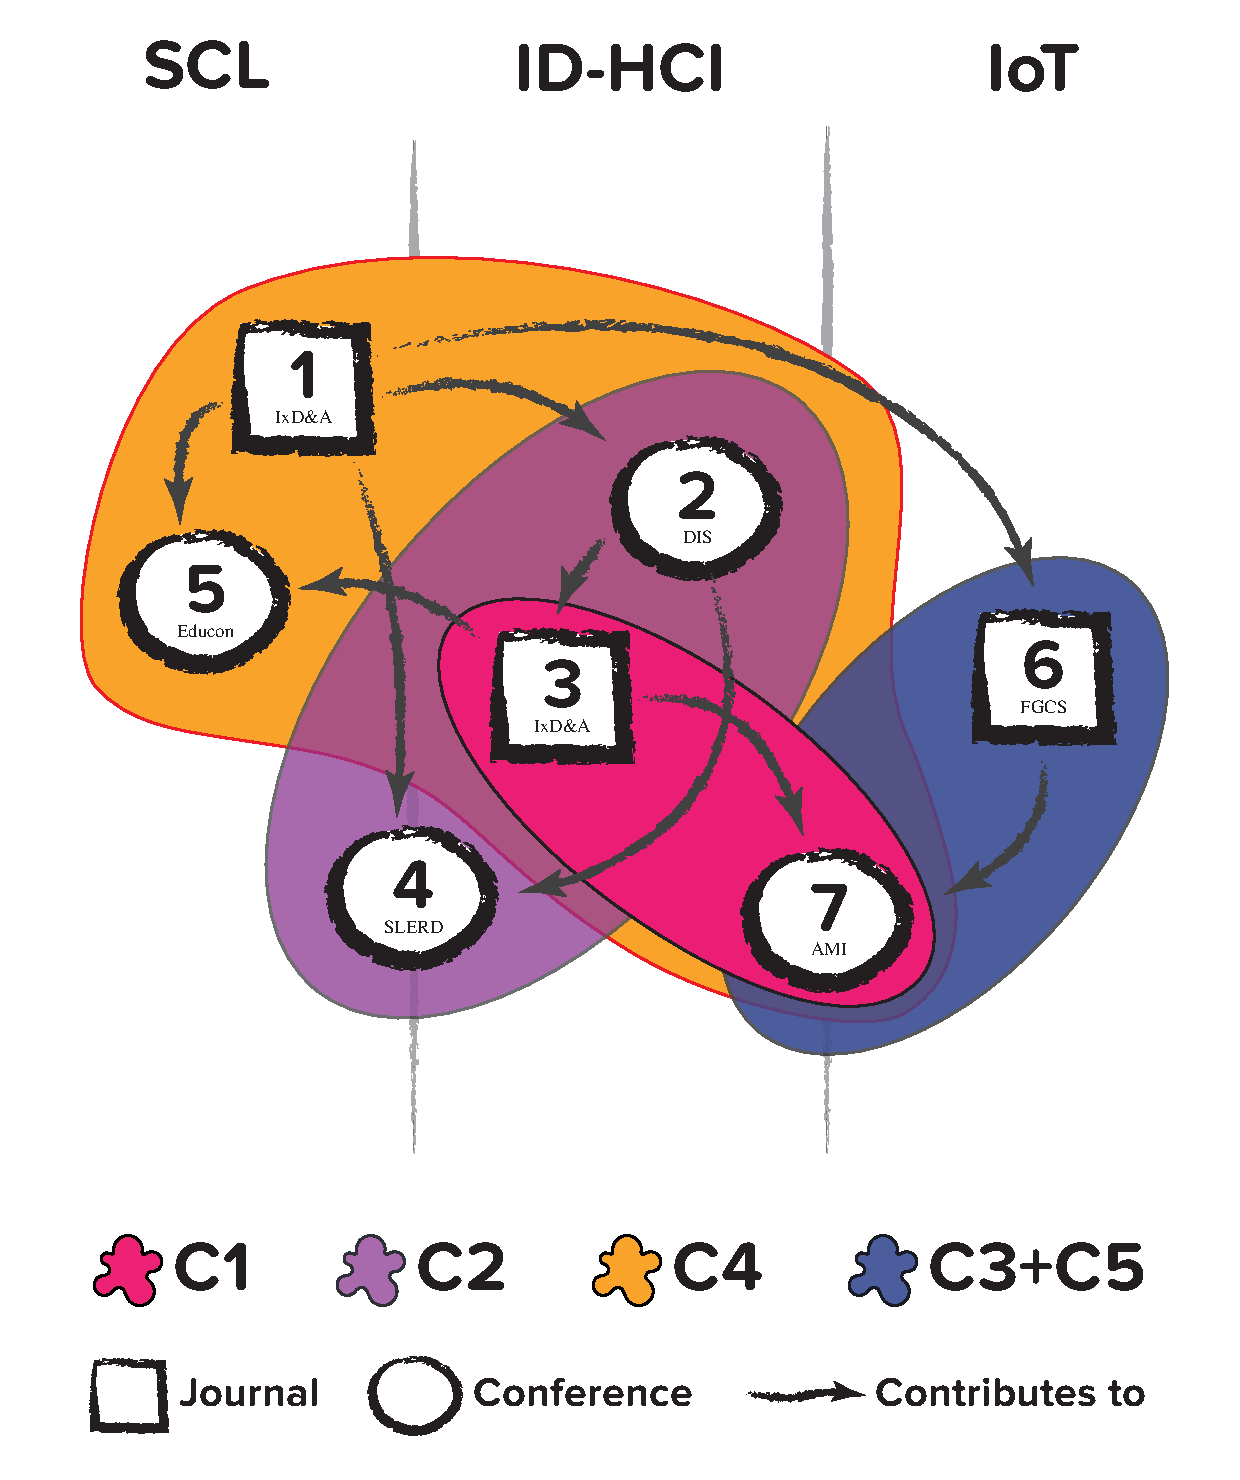
\includegraphics[width=\textwidth]{papers}
	\caption{A schema of the contributions. On top, from left to right: the domains of SCL, ID, HCI and IoT.}
	\label{fig:papers-contributions}
\end{figure}

\begin{table}[tbh]
	\centering 
	\caption{Mapping of contributions with papers.} 
	\label{tab:papers-and-contributions} 
	\smallskip
	\begin{tabular}{@{}lccccc@{}}
	\toprule
	  & C1 & C2 & C3 & C4 & C5 \\
	\midrule
	Paper 1 & & & & \textbullet & \\
	Paper 2 & & \textbullet & & \textbullet & \\
	Paper 3 & \textbullet & \textbullet & & \textbullet & \\
	Paper 4 & & \textbullet & & & \\
	Paper 5 & & & & \textbullet & \\
	Paper 6 & & & \textbullet & & \textbullet \\
	Paper 7 & \textbullet & & \textbullet & \textbullet & \textbullet \\
	\bottomrule 
	\end{tabular}
\end{table}


\section[C1: \Ci][Contribution 1]{C1: \Ci.}
\label{c1}

Contribution 1 is related to the theoretical definition, design and evaluation of an integrated framework supporting non-experts in idea generation and rapid prototyping of IoT applications based on augmented objects. In the context of this holistic process, the work presented in the thesis can be divided into two main blocks. The first one addresses the initial idea generation and design phases, where non-experts learn about the domain and generate an idea. The second block aims at creating a tangible prototype of the idea generated and includes the programming of the augmented object behaviour.
The process is tuned to be integrated, reusing the same conceptual building blocks during the different phases. It allows gradually building on the knowledge acquired, steadily supporting non-experts without demanding professional skills in any of the steps required. The definition of input/output primitives (Section~\ref{sec:integration-proto}) is an example of these conceptual building blocks that facilitate the transition between the design and prototyping phases. I designed and developed the majority of the input/output primitives that were used in the studies included in P3, P6 and P7, both in terms of cards included in the Tiles ideation toolkit and software of the RapIoT toolkit.
Special attention to the nature of this holistic process is reserved in P3 and P7, which also represent at best the work pertaining to each of the two blocks. For a detailed description of the complete framework, see Chapter~\ref{cha:iot-framework}.
Part of this contribution are also the lessons learned and the guidelines formalised as a result of my experience on the field (see P3~\S6 and P7~\S5, \S6).

This novel approach differs from the one adopted by most of the toolkits already available, which usually support either the design and brainstorming part or the prototyping and programming one, with no facilitation in bridging the two stages. A production-ready toolkit embracing this framework can be beneficial in education and design and for tangible exploration of creative ideas.


\section[C2: \Cii][Contribution 2]{C2: \Cii.}
\label{c2}

Contribution 2 of the thesis comprises new knowledge about how theoretical concepts of co-design and tangible user interaction (Chapter~\ref{cha:theory}) can inform the design, implementation and evaluation of a design and idea generation toolkit for IoT. The toolkit was developed during several design iterations to support non-experts in idea generation and design of IoT applications; its initial version is described in P2. The toolkit was designed to be frictionless and easy to adopt for users without previous knowledge of IoT or design methods. Some of the improvements developed during the first design iteration and the specialisation towards the smart city domain are described in P3. At the end of each design iteration, the artefacts were empirically evaluated, and the feedback gathered informed the following version of prototypes. The final artefact produced by the work related to C2 was a new version of the generic Tiles ideation toolkit and additional specialisations addressing IoT applications for reflective learning and smart cities. More in particular, I redesigned the cardboard (Fig.~\ref{fig:cardboard}), modified some of the already existing cards, designed and added new cards and card categories (P3~\S3) and added an extension to the storyboard and personas canvas to support IoT applications for reflective learning (P4~\S3). I used the insights gathered on the field to prepare a set of instructions to guide the users during group-based brainstorming and design activities. Starting from these instructions, I refined the \textit{playbook} reported on the cardboard, initially described in P2. The new \textit{playbook} was then successfully employed in the version of the toolkit used during P3, P4, P5 and P7. I developed and refined such guidelines to provide a toolkit that is self-supported and does not need direct supervision by experts to be used. In order to facilitate adoption, especially in educational contexts, I designed the process to be self-contained, short-lasting from start to finish and entertaining. The toolkit, the idea generation process and all the materials were open source and were made available for free under a creative commons licence.

The Tiles ideation toolkit supports co-design as a strategy to involve different stakeholders in the brainstorming phase of an IoT application. The group-based activity, the use of specific cards designed to spark creativity and reflection and the physicality of combining artefacts to define the seed of the idea all helped in provide a shared understanding of the problem and solution strategy, despite the diversities in skills and backgrounds of the participants. The toolkit is a viable instrument also for co-design workshops. Depending on the goal of the design workshop, a facilitator or expert might be necessary to support the users. This scenario emerged during the studies described in P4, where I specialised the toolkit towards IoT applications for reflective learning. Given the complexity of this approach for non-experts, a facilitator was needed to support the users during the workshops.

Contribution 2 can be a resource for researchers, designers, students and any user falling in the category of non-expert, who is interested in learning about IoT and generating ideas of IoT applications based on augmented objects and tangible interfaces. Although the toolkit was born to be generic, I subsequently specialised it for the smart city domain and for IoT application for reflective learning. This demonstrates its flexibility and the opportunity for it to be repurposed for other domains with limited effort.


\section[C3: \Ciii][Contribution 3]{C3: \Ciii.}
\label{c3}

The third contribution of the thesis includes the design, implementation and evaluation of an electronic and programming toolkit to prototype IoT ideas of augmented objects. The final prototypes produced are examples of tangible interfaces (Chapter~\ref{cha:theory}), and the toolkit itself is oriented into supporting rapid and tangible exploration of idea concepts. The RapIoT toolkit is designed to connect and build on the outcome of the brainstorming and design phases, covered by C2.
The RapIoT toolkit is composed of several hardware devices and software layers deployed in a cloud application, a development environment, a mobile app and a firmware for microcontrollers for embedded devices. For a more detailed description, see Chapter~\ref{cha:iot-framework}. The software structure of the toolkit is mainly described in P6, whereas a more extensive evaluation where non-experts created prototypes of augmented objects using the toolkit is reported in P7.
In order to allow non-experts to create a smart object and program its behaviour, the toolkit aimed to keep the entry barriers low, as in the preceding phases.
The toolkit includes electronic \textit{stickers} that can be attached to regular objects to provide sensing and actuation capabilities. Since several \textit{stickers} can be used in a single application, it is possible to prototype applications supporting distributed input and output, spread into several interconnected objects. I designed, produced and tested one of the two electronic \textit{stickers}, during two design iterations.
Ease of use and rapid deployment are guaranteed by the absence of any wire and the use of a simplified language for programming and by not requiring the installation of any software.
I contributed in writing part of the cloud software layer of RapIoT, I wrote from scratch the firmware of one of the \textit{stickers} and rewrote and extended the firmware of the second one. I supervised and directed the development of the mobile application, which was assigned as a project to a group of students.

Contribution 3 can provide valuable insights into how to design a toolkit for tangible exploration of ideas for non-experts. The RapIoT toolkit itself is released under a creative commons licence and is free to use. It can act as a resource for non-experts, designers, students and makers. Crafting a physical prototype is an enriching experience that conveys knowledge, builds experience and provides a tangible artefact to validate use cases and idea concepts. Artefacts can also represent a shared means to further develop the discussion and collaboration around the original idea.


\section[C4: \Civ][Contribution 4]{C4: \Civ.}
\label{c4}

The fourth contribution of the thesis is related to the educational outcome, mainly connected to the use of the Tiles ideation toolkit during school hours, in the context of SCL. The user studies described in most of the papers included in this thesis had a twofold purpose: (i) to evaluate a specific iteration of the toolkit design and (ii) to support the learning process of the students involved in the evaluation. These user studies involved students aged from 13 to 27. The ideation workshop was included in the programme of courses on IoT or design or performed as a standalone activity during school hours.
While collecting data on the aspects related to the toolkit, we were also able to extend the investigation towards the learning outcome of the idea generation and prototyping activities supported by the toolkits. We recorded good feedback in terms of increased knowledge about the challenges connected to smart cities, the definition of IoT and its design space and increased interest in programming and tinkering.

Contribution 4 provides guidelines and an overview of the lessons learned while deploying the toolkits for educational purposes. I assessed these two aspects in P7~\S5 to \S7, while a more elaborated evaluation protocol for the learning outcomes of the workshop was devised in P5.
During these studies, knowledge was gathered in adapting the creative activity to students of different ages and with diverse backgrounds.


\section[C5: \Cv][Contribution 5]{C5: \Cv.}
\label{c5}

The fifth contribution condenses the experience gathered in working with IoT design and prototyping toolkits and IoT systems in general. During the research activities described in this thesis, I put considerable effort in investigating and experimenting with different IoT technologies, software frameworks, sensors, microcontrollers and networking solutions. Some of the outlined challenges affecting modern IoT solutions were identified, and the vision for an improved IoT technical framework was drafted, inspired and supported by emerging movements, standards and publications targeting the same shortcoming. Some of these challenges were broad and generic. However, whenever possible, the IoT model I envisioned and described in Chapter~\ref{cha:iot-framework} was specialised to address the requirements dictated by having non-experts as target users.

Contribution 5 provides the description of an IoT technical framework to support rapid prototyping of smart objects, having non-experts as target users. The envisioned solutions aim to be open, accessible and future-proof, following the philosophy adopted by the web. See Chapter~\ref{cha:iot-framework} for a more detailed description of the framework.
\chapter{Evaluation}
\label{cha:evaluation}

This chapter describes the evaluation of the contributions presented in Chapter~\ref{cha:contributions} in connection with the research questions. In addition, validity threats are discussed, and the external impact of the research work is summarised.


\section{Evaluation of Research Questions}

\subsection*{MRQ: \MRQ}
\label{mrq}
The main research question is answered by Contributions 1, 2 and 3. Using co-design workshops, it was demonstrated how concepts from theories in tangible user interaction can be deployed into a suite of tools, applications, methods and artefacts. This integrated suite was demonstrated to be useful and effective in supporting non-experts in generating ideas and prototypes of tangible interfaces and smart augmented objects. Different tools addressed different phases of the process, whereas a holistic framework was designed to support the users throughout the whole journey.

\subsection*{RQ1: \RQi}
\label{rq1}
The answer to the first research question is provided by Contribution 1. The work included in C1 describes in detail the tools and co-design methods employed during the phases included in the process defined by the Tiles IoT framework. Emphasis is placed on how the transition between the idea and the prototype is facilitated, maintaining a complexity level suitable for non-experts.

\subsection*{RQ2: \RQii}
\label{rq2}
This research question is answered by Contributions 2 and 4. C2 includes the studies where the Tiles ideation toolkit was firstly introduced and the ones where it was specialised in the domains of smart cities and IoT applications for reflective learning. C4 explores how the toolkits and the methods developed can be employed to support SCL.

\subsection*{RQ3: \RQiii}
\label{rq3}
This research question is answered by Contribution 3 and 5. A technical architecture to support prototyping of IoT applications is described in C5. Its implementation into a rapid prototyping toolkit is then proposed and evaluated during prototyping workshops with non-expert users. C3 focuses on these phases of programming, prototyping and tangible exploration of ideas.


\section{Evaluation of the Research Approach in Field Studies}
\label{evaluation-of-research-approach}

The research approach employed during the investigation described in this thesis is evaluated here. Validity and reliability issues \autocites{yin_case_2017}{riege_validity_2003} are also discussed.

Criteria were established for judging the quality of the case study method \autocite{riege_validity_2003}. Several tests and techniques were synthesised for establishing validity and reliability in case study research.
In the following section, the research approach is evaluated following the guidelines and design tests reported by Riege \autocite*{riege_validity_2003}; however, not all the tests devised by Riege apply to the studies included in this thesis.

\subsection{Construct Validity}
\label{construct-validity}
Construct validity evaluates whether appropriate operational measures have been adopted for the theoretical concepts being researched.
Collecting data using multiple data sources increases construct validity and protects against researcher bias \autocites{perakyla_reliability_1998}{flick_triangulation_1992}. Converging findings emerged when analysing different sources through triangulation. This has been the case for the data collected during the evaluation workshops. We collected quantitative and qualitative data through questionnaires, structured interviews, observations, video and audio recordings and analysis of the artefacts produced. Chains of evidence in the data \autocites{griggs_analysing_1987}{hirschman_humanistic_1986} were highlighted when summarising the outcome of the data analysis process.

The number of participants involved in the studies added up to more than 500. A fraction of them were involved in the studies presented in this thesis. Significant experience was gathered in the process, such experience contributed to the definition of theories and in providing insights while analysing qualitative and quantitative data.
The size of the data sample allowed for some statistical analysis, but I looked for confirmation in the qualitative data before formalising the results. Given the number of human factors involved, this strategy was demonstrated to be more robust and allowed for better interpretation of the data collected.

During the studies, researchers had close and direct personal contact with the organisations and users involved. Effort was then made to refrain from subjective judgements during the periods of research design and data collection, to enhance construct validity.

Each of the studies was limited to one or two sessions, lasting usually two to three hours each. It was, therefore, not possible to prove long-term effects for the tools developed.

\subsection{Internal Validity}
Internal validity, as traditionally known in quantitative research, refers to the establishment of cause-and-effect relationships, while the emphasis on constructing an internally valid research process in case study research lies in establishing phenomena in a credible way \autocite{riege_validity_2003}. Researchers should not only highlight major patterns of similarities and differences between the experience of the respondents and their beliefs but also try to identify what components are significant for those examined patterns and what mechanisms produced them.

Data from the field studies included in the papers presented in this thesis were checked cross-case to assess the internal coherence of findings \autocite{miles_qualitative_1994}. Illustrations and diagrams eased this task, allowing the identification and evaluation of evidence, cross-checking within-case and cross-case \autocite{yin_case_2017}.

During field studies, it was sometimes required to deviate from the agreed protocol because of unpredictable events. In addition, it was difficult to replicate the same exact conditions because of the human factors involved and the lack of control over some of the variables. Workshops in the classroom were often limited in time, involved a variable number of students and took place at different times of the day.

Despite the challenges, I was able to gather enough evidence to complete the design work. The experience matured was helpful in extracting valuable know-how from noisy data sets.

\subsection{External Validity}
External validity is concerned with the extrapolation of particular research findings beyond the immediate form of inquiry to the general.

While quantitative research, for example, using surveys aims at statistical generalisation and synthesis as methods to pursue external validity, case studies rely on analytic generalisation, whereby particular findings are generalised to some broader theory. The focus lies on an understanding and exploration of constructs, that is, usually the comparison of initially identified and/or developed theoretical constructs and the empirical results of single or multiple case studies \autocite{riege_validity_2003}.

In order to increase the external validity, several techniques were employed. The logic of the case study was replicated across different domains \autocites{eisenhardt_building_1989}{parkhe_messy_1993}: most of the workshops involved students, but the tools were evaluated also with other target users (e.g. in P4), including researchers, employees from the municipality, entrepreneurs, programmers and freelancers.

The boundaries and scope of the research were defined in the research design phase \autocite{marshall_designing_2014}. The outcome for each of the phases covered by the toolkits was clearly defined, as well as the target users of the toolkits and their attributes (see Chapter~\ref{cha:iot-framework} for details).

Lastly, comparison of evidence with the extant literature in the domain of interest helped in clearly outlining the contributions and in generalising, always within the scope and boundaries of the research \autocite{yin_case_2017}.

\subsection{Reliability}
Reliability refers to the demonstration that the operations and procedures of the research inquiry can be repeated by other researchers who then achieve similar findings; that is, the extent of findings can be replicated assuming that, for example, the interviewing techniques and procedures remain consistent \autocite{riege_validity_2003}.

In case study research, this can raise problems as people are not as static as measurements used in quantitative research, and even if researchers were concerned about ensuring that others can precisely follow each step, the results may still differ. Indeed, data on real-life events, which were collected by different researchers, may not converge into one consistent picture. However, possible differences also can provide a valuable additional source of information about the cases investigated \autocite{riege_validity_2003}.

The techniques used to increase reliability included the recording of observations and actions as concretely as possible \autocite{lecompte_problems_1982}, the use of pilot studies to develop and refine the case study protocol \autocites{eisenhardt_building_1989}{mitchell_industrial_1993}{yin_case_2017}, the use of multiple researchers who continually communicate about methodological decisions \autocite{lecompte_problems_1982}, the mechanical recording of data \autocite{nair_using_1995}, the development of a case study database to organise and document the mass of collected data \autocite{lincoln_naturalistic_1985} and finally the use of peer review and examination \autocite{lecompte_problems_1982}.

Repeatability can be demonstrated by the existence of external publications employing the Tiles ideation toolkit in contexts similar to the ones presented in the papers included in this thesis (see Section~\ref{sec:exploitation} for details). In some cases, the ideation process directing the use of the Tiles cards was modified or extended (e.g. removing the cardboard). The results reported, however, are aligned with the findings presented in this thesis.

Relative to repeatability, limitations might affect the prototyping phase. This phase, in fact, was evaluated and tested only internally during the last months of my PhD. External adoption and independent evaluations of the prototyping toolkit are not yet possible because of the early stage of development of the hardware and software stacks.


\section{Exploitation and External Impact of Research}
\label{sec:exploitation}

The Tiles ideation toolkit has been largely and independently employed in the research, governance, industry and education sectors from institutions in Europe, America, Asia and Australia.
A few examples are the works of 
Gennari et al. \autocite*{gennari_design_2017}, Sintoris at al. \autocite*{sintoris_out_2018}, Avouris et al. \autocite*{avouris_designing_2018} and  Zhai et al. \autocite*{zhai_co-sleep_2018}. The Tiles ideation toolkit was also selected by an independent group of researchers to support an ideation and rapid prototyping workshop during the CHI Conference on Human Factors in Computing Systems, in 2018 \autocite{angelini_internet_2018-1}.

The Tiles ideation toolkit was employed at NTNU during workshops as part of the master-level university courses in \textit{Cooperation Technology and Social Media} (TDT4245) at the Department of Computer Science, \textit{Prototyping Interactive Media} (TPD4126) at the Department of Design and \textit{Design of Communicating Systems} (TTM4115) at the Department of Information Security and Communication Technology.

A small community formed around the Tiles project, with particular emphasis on the Tiles ideation toolkit, but with high interest also in the tools for programming and rapid prototyping. Around 10 groups approached us directly to ask for guidance, customisation and assistance in running the workshop. Thanks to the open-source licence of the cards, cardboard and workshop technique, several contributed to creating extensions for different domains, like smart buildings, or creating typesets to ease printing and collaboration tasks.

A company was started to refine and integrate the prototypes produced during the research activities, with the objective of developing a kit suitable for distribution.
A Kickstarter campaign is currently scheduled to crowdfund the first production batch of the Tiles ideation toolkit.

\chapter{Conclusions and Future Work}
\label{cha:conclusions}


The work described in this thesis focused on enabling non-experts to generate ideas and prototypes of IoT applications involving augmented objects and tangible interfaces.

The main research method adopted was design science research. Several user studies were performed to evaluate the tools developed and the creative process supporting the users from idea generation to prototyping.
The work was grounded in the literature about SCL, co-design, tangible interfaces and user-centred design.
Prototypes and tools were produced in the form of a design toolkit, electronic devices for object augmentation, mobile applications and a software toolkit. Each of them was developed through multiple design iterations, producing various intermediate versions at different levels of fidelity.
The scientific work has been published in peer-reviewed journals and conference proceedings, and seven of these publications were included in this thesis.

The research questions were answered by five contributions, hereafter summarised in a set of conclusions that also delineate future work. 


\section*{Conclusion 1}

The experience matured and the tools produced can be used to support non-experts in learning about IoT and smart cities, generating an IoT application idea starting from a real problem and prototyping such idea into a programmable demonstrator.
This emerged as a complex process to define and evaluate, involving a diverse set of skills that require team effort in the areas of learning, social sciences, programming, networking protocols, electronics and embedded hardware and software.
Prototypes covering each of these areas were created and successfully evaluated for their impact on supporting non-experts throughout the whole creative process (P3, P7).
Lessons learned and feedback gathered drove the definition of new theories and guidelines (P7).

Additional work is required to finalise the design of the tools, especially the ones covering the prototyping phase. Given the positive feedback collected, future work will generalise tools and methods to cover other application domains in addition to smart cities.


\section*{Conclusion 2}

The holistic IoT ideation process, spanning from brainstorming to prototyping, already covered in C1, was investigated in two phases. The first phases covered the process of idea generation and design, during which the users familiarised with the application domain and the solution space and produced an IoT application idea while brainstorming in group-based workshops. These activities were supported through the Tiles ideation toolkit, a card-based toolkit developed and evaluated in multiple iterations (P2, P3 and P4).
We received excellent feedback during the user studies, and the toolkit was independently adopted by schools and institutions all over the world. We experimented with extensions targeting specific domains and learning strategies (P4).

Future work might include the internationalisation of the cards and the cardboard, in order to promote adoption in non-English-speaking countries. Minor enhancements in the card decks are also planned to further reduce the complexity and increase the ease of use. Finally, new cards could eventually be created to specialise the toolkit for specific application domains, like healthcare or smart homes.


\section*{Conclusion 3}

The final phases of the process covered in C1 address rapid prototyping and tangible exploration of ideas. These phases were designed to integrate with the idea generation phase and to allow non-experts to produce a prototype of the augmented objects envisioned. The RapIoT toolkit (P6) supported the technical infrastructure employed by the users during programming and prototyping. The technologies include a cloud development environment, an application for mobile devices, a communication protocol and a firmware for embedded devices. The process and the technical solutions were successfully evaluated (P7) through user studies where non-experts developed and programmed prototypes of augmented objects.

Future work will be oriented towards revising the technical tools in order to adopt open standards, increase the efficiency and simplify the programming paradigm and the deployment procedure.


\section*{Conclusion 4}

While running the field studies, the educational potential of the Tiles ideation toolkit naturally emerged. A side research line was then dedicated to exploring more systematically the outcome in terms of learning (P5). When the Tiles ideation toolkit was employed as a learning tool, we received good feedback in terms of improved knowledge about IoT and smart cities. The combination between technology and domain expertise was also beneficial in conveying SCL (P2, P5 and P7).

Future improvements to support the learning outcome can include better integration into the curricula of the schools. Internationalisation of the tools might also benefit the younger students, who occasionally find it difficult to understand the terminology employed without being assisted by the teacher.


\section*{Conclusion 5}

In the process of designing, developing and evaluating the tools and methods described in this thesis, theoretical and technical knowledge about the IoT domain was acquired. Design and technical challenges became evident while experimenting and were later confirmed by reviewing the relevant domain literature (Chapter~\ref{cha:iot-framework}). Based on such literature, a descriptive draft of an IoT framework was redacted. This framework aims on the one hand to overcome the identified challenges and on the other hand to extend the support towards a concept of IoT that includes humans in the loop, standardising tangible interaction primitives and object manipulation. Future work will include a formal definition of the framework and an initial implementation that integrates with the architecture described in C3.

\bigskip
\begin{center}
\noindent\rule{8cm}{0.4pt}    
\end{center}
\bigskip

In conclusion, this thesis has developed knowledge and tools about a holistic process supporting non-experts in learning, ideation and prototyping of IoT applications for augmented objects. My investigation used SCL as a domain case, but the basis for generalising the theories and technologies developed has been settled.
Commercial exploitation is currently being explored, and future work aims to improve the prototypes created and to explore new application domains while maintaining the theoretical foundations that backed the work presented here.

\appendix
\backmatter
\printbibliography[title=References]

\makeatletter
\def\pagenumbering#1{%
  \gdef\thepage{\csname @#1\endcsname \c@page}}
\makeatother

\mainmatter
\part[Part II]{Research Papers}
\pagenumbering{gobble}
\pagestyle{cleared}
\chapter*{Research Papers}
\begin{small}
\begin{enumerate}[label=\numberingI{\textbf{P\arabic*}}]
    \item Gianni, Francesco, and Monica Divitini (2016) \textbf{\enquote{Technology-Enhanced Smart City Learning: A Systematic Mapping of the Literature.}} \emph{Interaction Design and Architecture(s) Journal - IxD\&A} 27:28--43.
    
    \item Mora, Simone, Francesco Gianni, and Monica Divitini (2017) \textbf{\enquote{Tiles: A Card-Based Ideation Toolkit for the Internet of Things.}} In: Proceedings of the 2017 Conference on Designing Interactive Systems. DIS 2017. 587--598. Edinburgh, United Kingdom: ACM.
    
    \item Gianni, Francesco, and Monica Divitini (2018) \textbf{\enquote{Designing IoT Applications for Smart Cities: Extending the Tiles Ideation Toolkit.}} \emph{Interaction Design and Architecture(s) Journal - IxD\&A} 35:100--116.
    
    \item Gianni, Francesco, Lisa Klecha, and Monica Divitini (2019) \textbf{\enquote{Tiles-Reflection: Designing for Reflective Learning and Change Behaviour in the Smart City.}} In: The Interplay of Data, Technology, Place and People for Smart Learning. SLERD 2018. \emph{Smart Innovation, Systems and Technologies} 95:70--82. Aalborg, Denmark: Springer, Cham.
   
    \item Mavroudi, Anna, Monica Divitini, Francesco Gianni, Simone Mora and Dag R. Kvittem (2018) \textbf{\enquote{Designing IoT Applications in Lower Secondary Schools.}} In: Proceedings of IEEE Global Engineering Education Conference. EDUCON 2018. 1120--1126. Tenerife, Spain: IEEE.
    
    \item Gianni, Francesco, Simone Mora, and Monica Divitini (2018) \textbf{\enquote{RapIoT Toolkit: Rapid Prototyping of Collaborative Internet of Things Applications.}} \emph{Journal of Future Generation Computer Systems.} Elsevier.
    
    \item Gianni, Francesco, Simone Mora, and Monica Divitini (2018) \textbf{\enquote{Rapid Prototyping Internet of Things Applications for Augmented Objects: The Tiles Toolkit Approach.}} In: Ambient Intelligence. AmI 2018. \emph{Lectures Notes in Computer Science.} 11249:204--220. Larnaca, Cyprus: Springer, Cham.
\end{enumerate}
\end{small}

%PAPER 1
\cleardoublepage
\begin{flushright}
\textsc{\huge Paper 1}
\end{flushright}
\vspace{3cm}
\begin{center}
	\begin{framed}
		{\Large \textbf{Technology-Enhanced Smart City Learning:\\ A Systematic Mapping of the Literature}}
		
		\medskip
		Francesco Gianni and Monica Divitini
		
		\medskip		
		\emph{Interaction Design and Architecture(s) Journal -- IxD\&A}
	\end{framed}	
\end{center}

\vspace{9cm}


\includegraphics[height=20pt]{by-nc-nd}\\
{\scriptsize Copyright \textcircled{c} 2019. This manuscript version is made available under the \textbf{CC-BY-NC-ND 4.0} license.}\\
{\tiny https://creativecommons.org/licenses/by-nc-nd/4.0/}\\

\includegraphics[height=13pt]{OA} {\scriptsize -- IxD\&A is a Gold Open Access (OA) Journal.}
\cleardoublepage
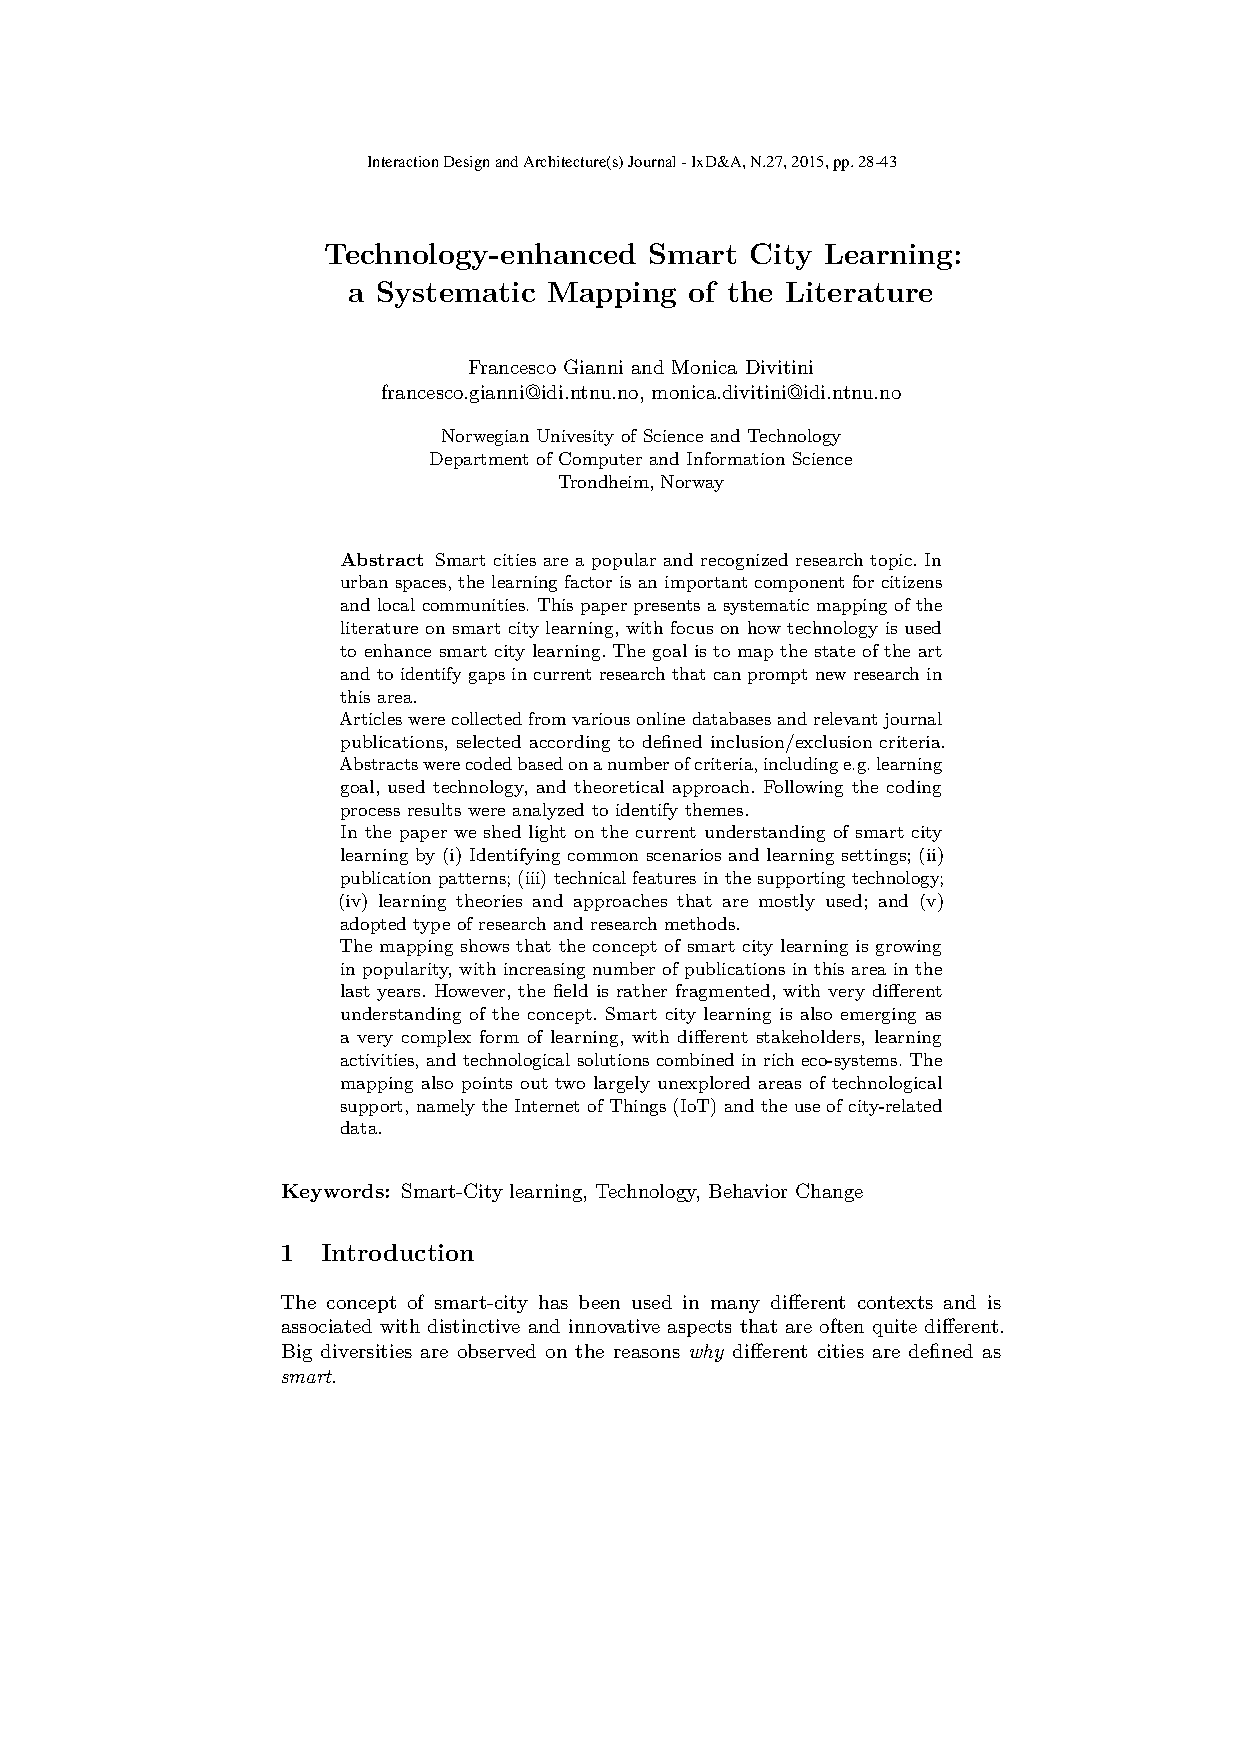
\includepdf[pages=-, noautoscale=true, scale=1, offset=5mm -5mm]{./papers_published/P1.pdf}

%PAPER 2
\cleardoublepage
\begin{flushright}
\textsc{\huge Paper 2}
\end{flushright}
\vspace{3cm}
\begin{center}
	\begin{framed}
		{\Large \textbf{Tiles: A Card-Based Ideation Toolkit\\ for the Internet of Things}}
		
		\medskip
		Simone Mora, Francesco Gianni and Monica Divitini
		
		\medskip		
		\emph{In: Proceedings of the 2017 Conference on Designing Interactive Systems (DIS)}
	\end{framed}
\end{center}

\vspace{10cm}

{\scriptsize Reprinted with kind permission from the Association for Computing Machinery (ACM).}\\
{\tiny DOI: https://doi.org/10.1145/3064663.3064699}
\cleardoublepage
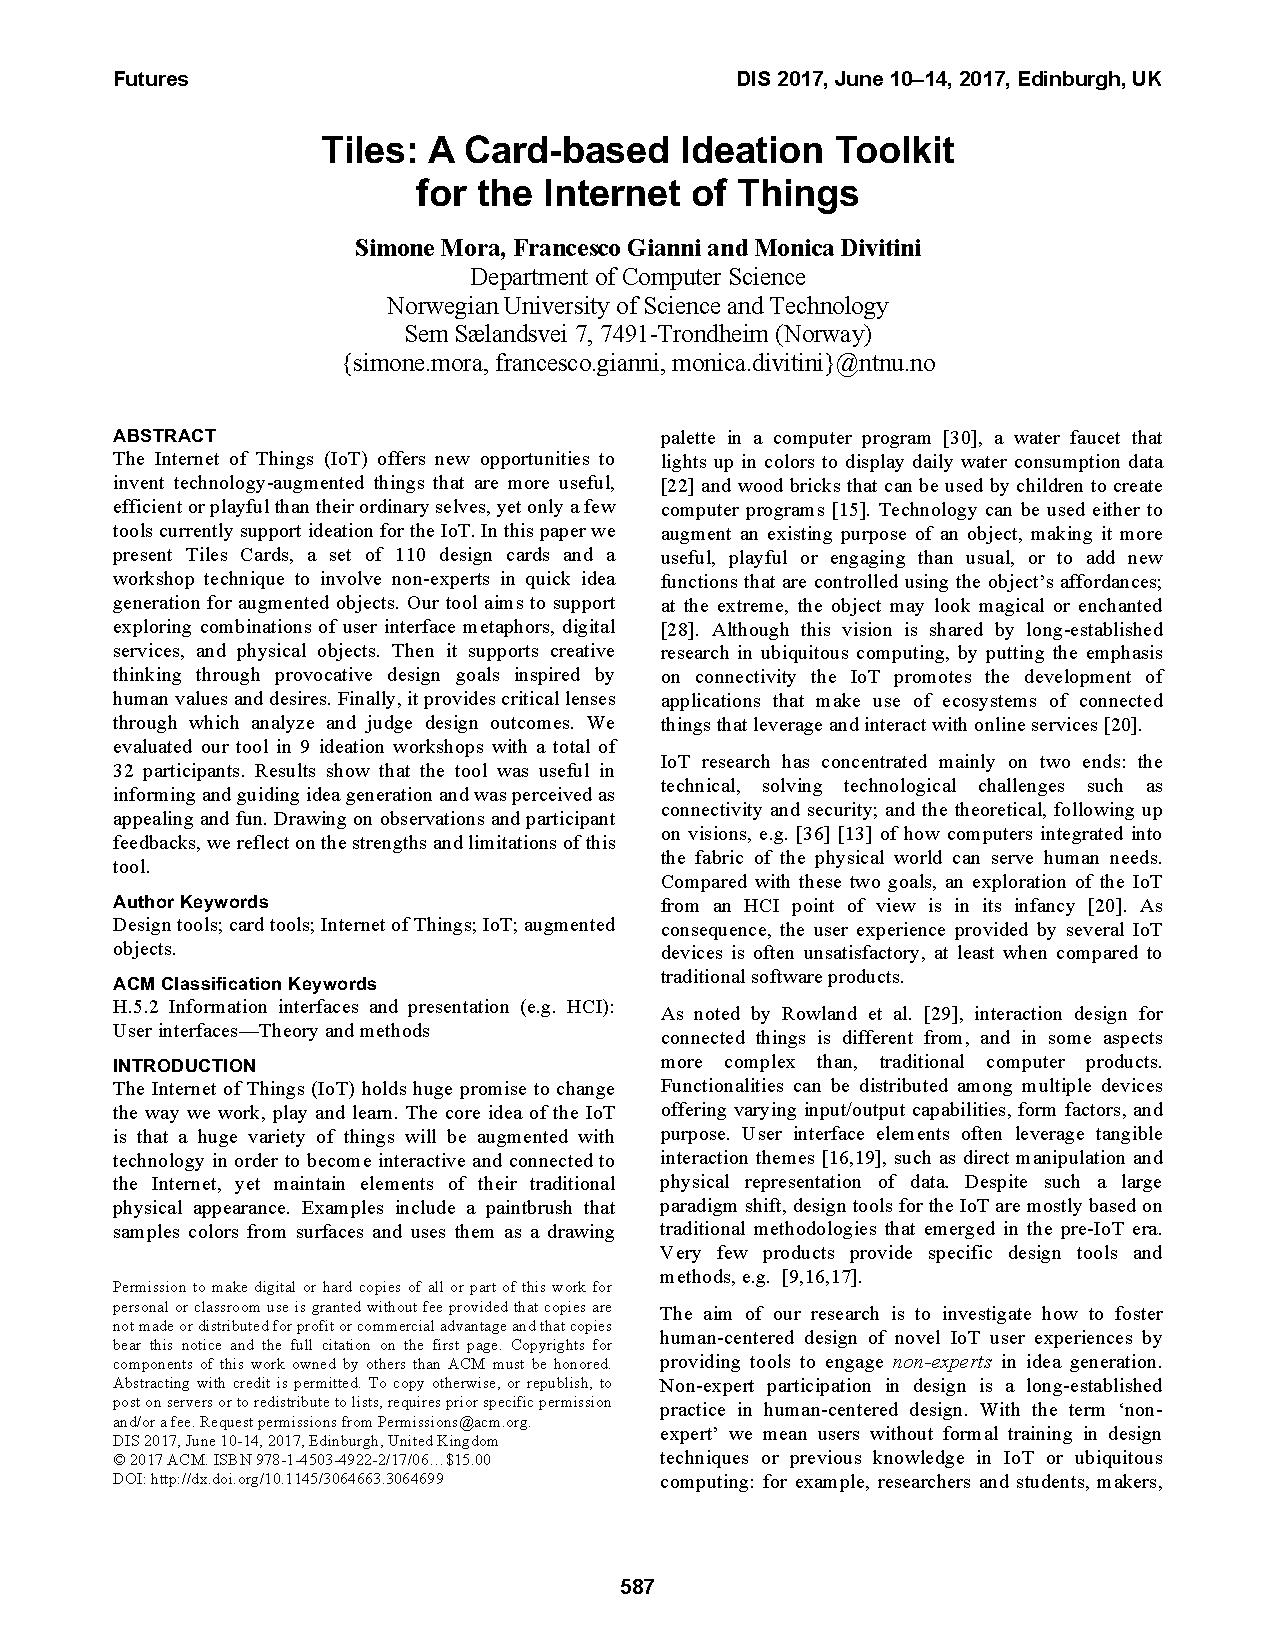
\includepdf[pages=-, noautoscale=true, scale=0.73, offset=5mm 0mm]{./papers_published/P2.pdf}

%PAPER 3
\cleardoublepage
\begin{flushright}
\textsc{\huge Paper 3}
\end{flushright}
\vspace{3cm}
\begin{center}
	\begin{framed}
		{\Large \textbf{Designing IoT Applications for Smart Cities:\\ Extending the Tiles Ideation Toolkit}}
		
		\medskip
		Francesco Gianni and Monica Divitini
		
		\medskip
		\emph{Interaction Design and Architecture(s) Journal -- IxD\&A}
	\end{framed}
\end{center}

\vspace{9cm}


\includegraphics[height=20pt]{by-nc-nd}\\
{\scriptsize Copyright \textcircled{c} 2019. This manuscript version is made available under the \textbf{CC-BY-NC-ND 4.0} license.}\\
{\tiny https://creativecommons.org/licenses/by-nc-nd/4.0/}\\

\includegraphics[height=13pt]{OA} {\scriptsize -- IxD\&A is a Gold Open Access (OA) Journal.}
\cleardoublepage
\includepdf[pages=-, noautoscale=true, scale=1, offset=5mm -5mm]{./papers_published/P3_thesis_edit.pdf}

%PAPER 4
\cleardoublepage
\begin{flushright}
\textsc{\huge Paper 4}
\end{flushright}
\vspace{3cm}
\begin{center}
	\begin{framed}
		{\Large \textbf{Tiles-Reflection: Designing for Reflective Learning and Change Behaviour in the Smart City}}
		
		\medskip
		Francesco Gianni, Lisa Klecha, and Monica Divitini
		
		\medskip
		\emph{In: The Interplay of Data, Technology, Place and People for Smart Learning (SLERD)}
	\end{framed}	
\end{center}

\vspace{10cm}

{\scriptsize Reprinted by permission from Springer International Publishing AG: Springer Nature -- The Interplay of Data, Technology, Place and People for Smart Learning. Knoche H., Popescu E., Cartelli A., {\tiny \textcircled{c} 2019.}}
\cleardoublepage
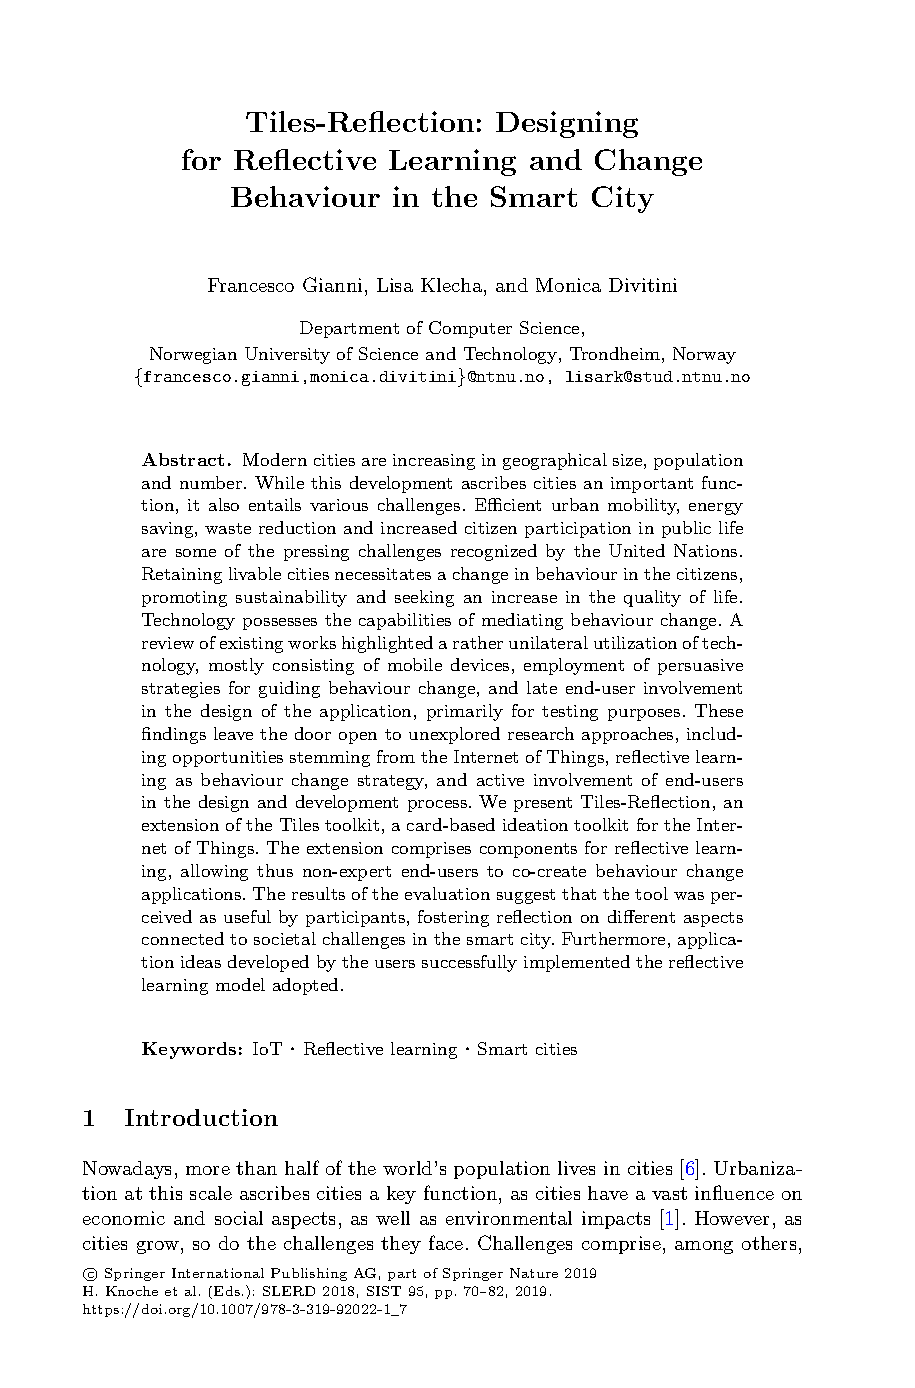
\includepdf[pages=-, noautoscale=true, scale=1, offset=7mm 0mm]{./papers_published/P4_thesis_edit.pdf}


%PAPER 5
\cleardoublepage
\begin{flushright}
\textsc{\huge Paper 5}
\end{flushright}
\vspace{3cm}
\begin{center}
	\begin{framed}
		{\Large \textbf{Designing IoT Applications in Lower Secondary Schools}}
		
		\medskip
		Anna Mavroudi, Monica Divitini, Francesco Gianni,\\ Simone Mora and Dag R. Kvittem
		
		\medskip
		\emph{In: Proceedings of IEEE Global Engineering Education Conference (EDUCON)}
	\end{framed}	
\end{center}

\vspace{9cm}

{\scriptsize \textcircled{c} 2019 IEEE. Reprinted, with permission, from: A. Mavroudi, M. Divitini, F. Gianni, S. Mora and D. R. Kvittem, \enquote{Designing IoT applications in lower secondary schools}, 2018 IEEE Global Engineering Education Conference (EDUCON), Tenerife, 2018, pp. 1120-1126.}\\
{\tiny DOI: https://doi.org/10.1109/EDUCON.2018.8363355}
\cleardoublepage
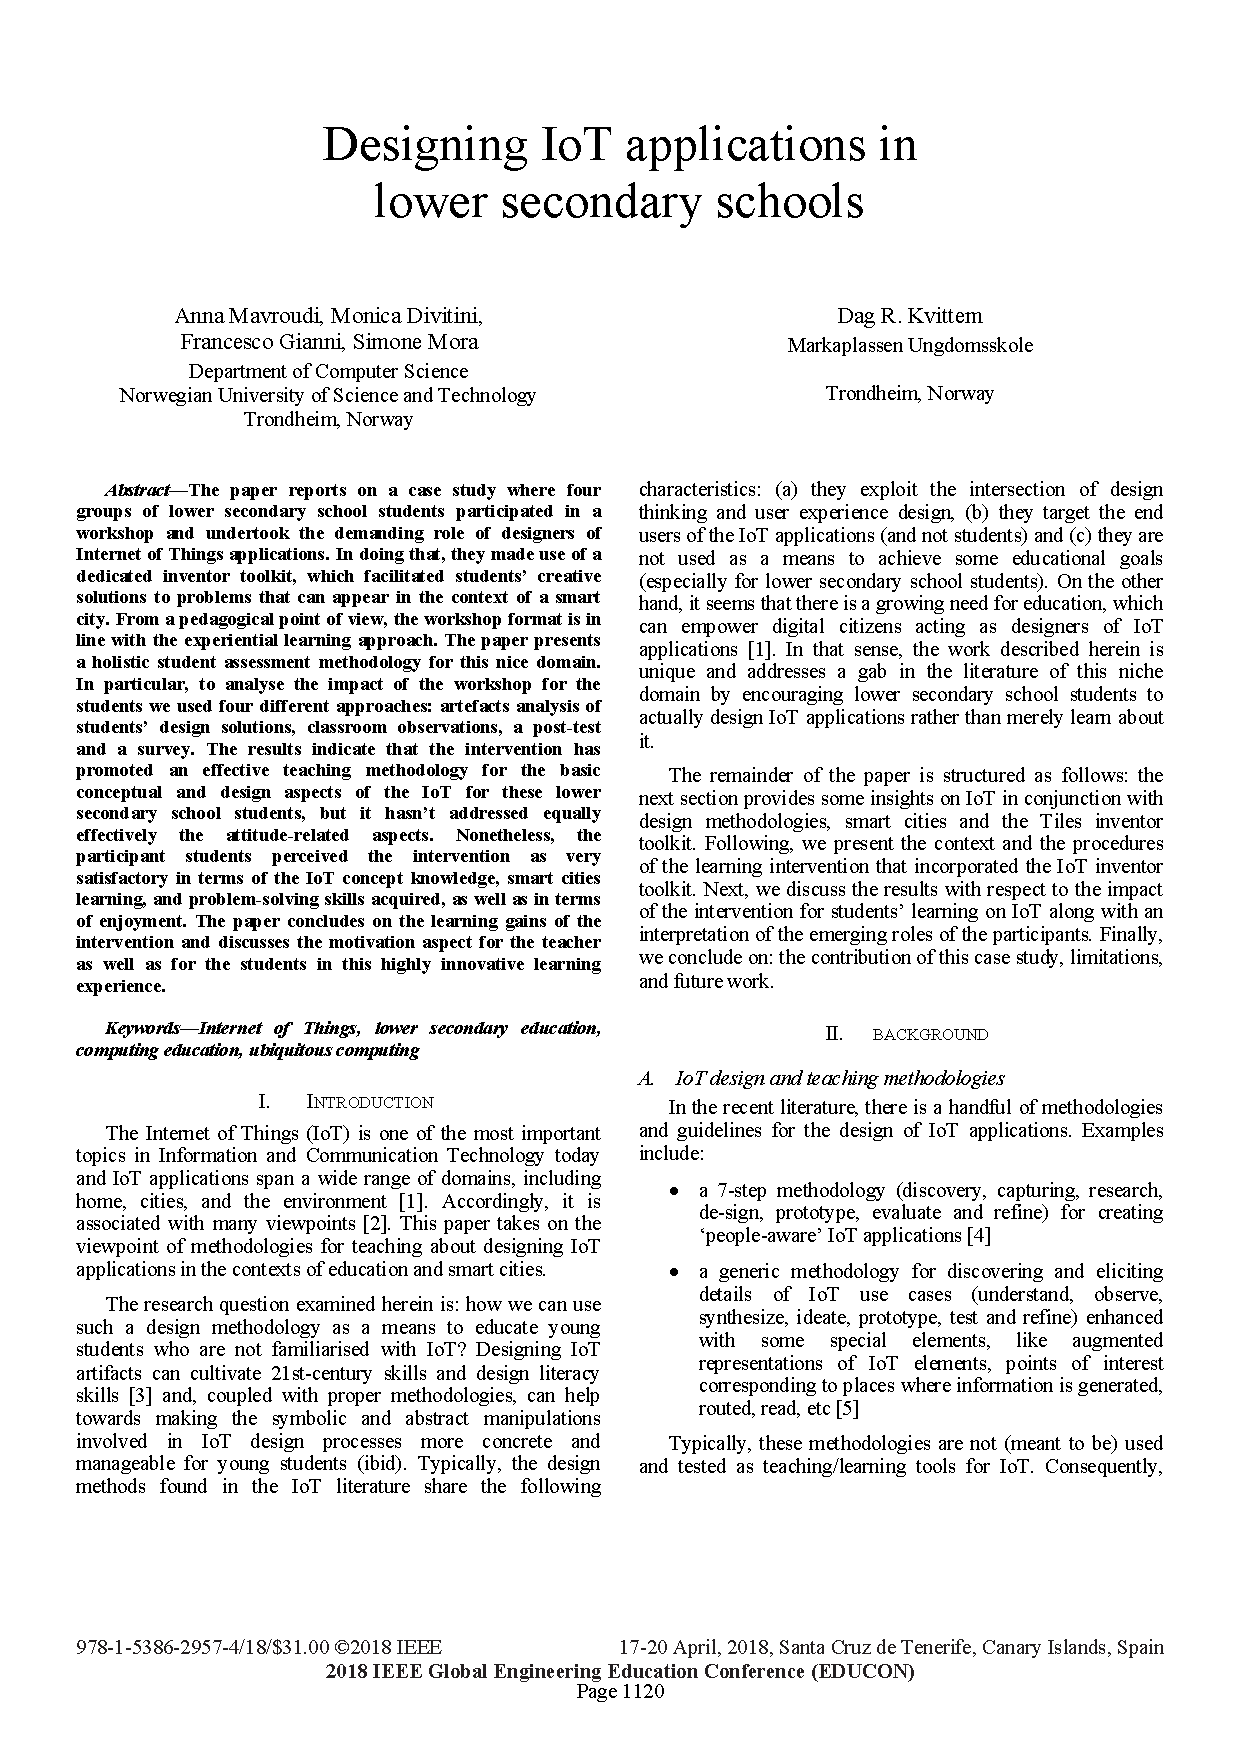
\includepdf[pages=-, noautoscale=true, scale=0.7, offset=6mm 0mm]{./papers_published/P5_thesis_edit.pdf}


%PAPER 6
\cleardoublepage
\begin{flushright}
\textsc{\huge Paper 6}
\end{flushright}
\vspace{3cm}
\begin{center}
	\begin{framed}
		{\Large \textbf{RapIoT Toolkit: Rapid Prototyping of Collaborative Internet of Things Applications}}	
		\medskip
		
		Francesco Gianni, Simone Mora, and Monica Divitini
		
		\medskip
		\emph{Journal of Future Generation Computer Systems}
	\end{framed}	
\end{center}

\vspace{10cm}

{\scriptsize \textcircled{c} 2019 Elsevier B.V. Reprinted, with permission, from: F.Gianni, et al., RapIoT toolkit: Rapid prototyping of collaborative Internet of Things applications, Future Generation Computer Systems (2018), https://doi.org/10.1016/j.future.2018.02.030}
\cleardoublepage
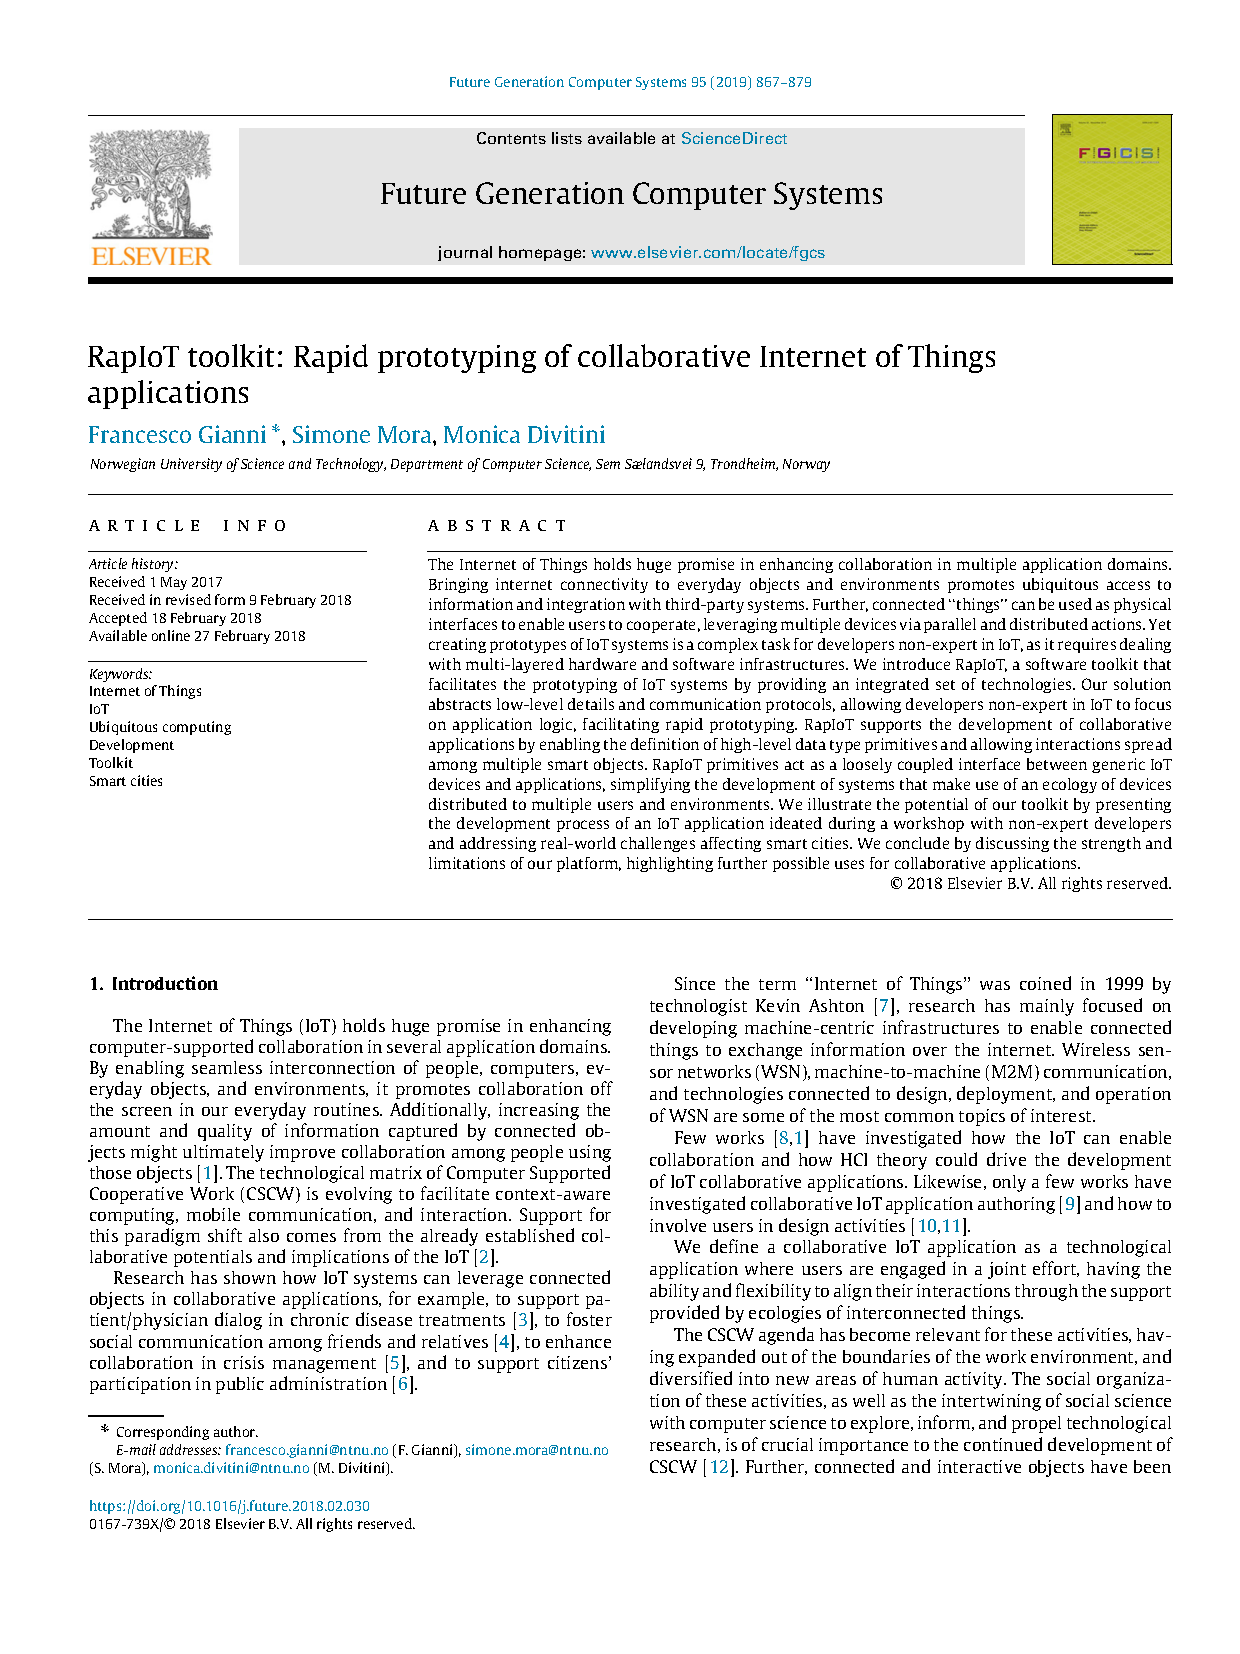
\includepdf[pages=-, noautoscale=true, scale=0.7, offset=5mm 0mm]{./papers_published/P6.pdf}


%PAPER 7
\cleardoublepage
\begin{flushright}
\textsc{\huge Paper 7}
\end{flushright}
\vspace{3cm}
\begin{center}
	\begin{framed}
		{\Large \textbf{Rapid Prototyping Internet of Things Applications for Augmented Objects: The Tiles Toolkit Approach}}	
		\medskip
		
		Francesco Gianni, Simone Mora, and Monica Divitini
		
		\medskip		
		\emph{In: Ambient Intelligence (AmI)}
	\end{framed}	
\end{center}

\vspace{10cm}

{\scriptsize Reprinted by permission from Springer International Publishing AG: Springer Nature -- Ambient Intelligence. Kameas A., Stathis K., \textcircled{c} 2019.}
\cleardoublepage
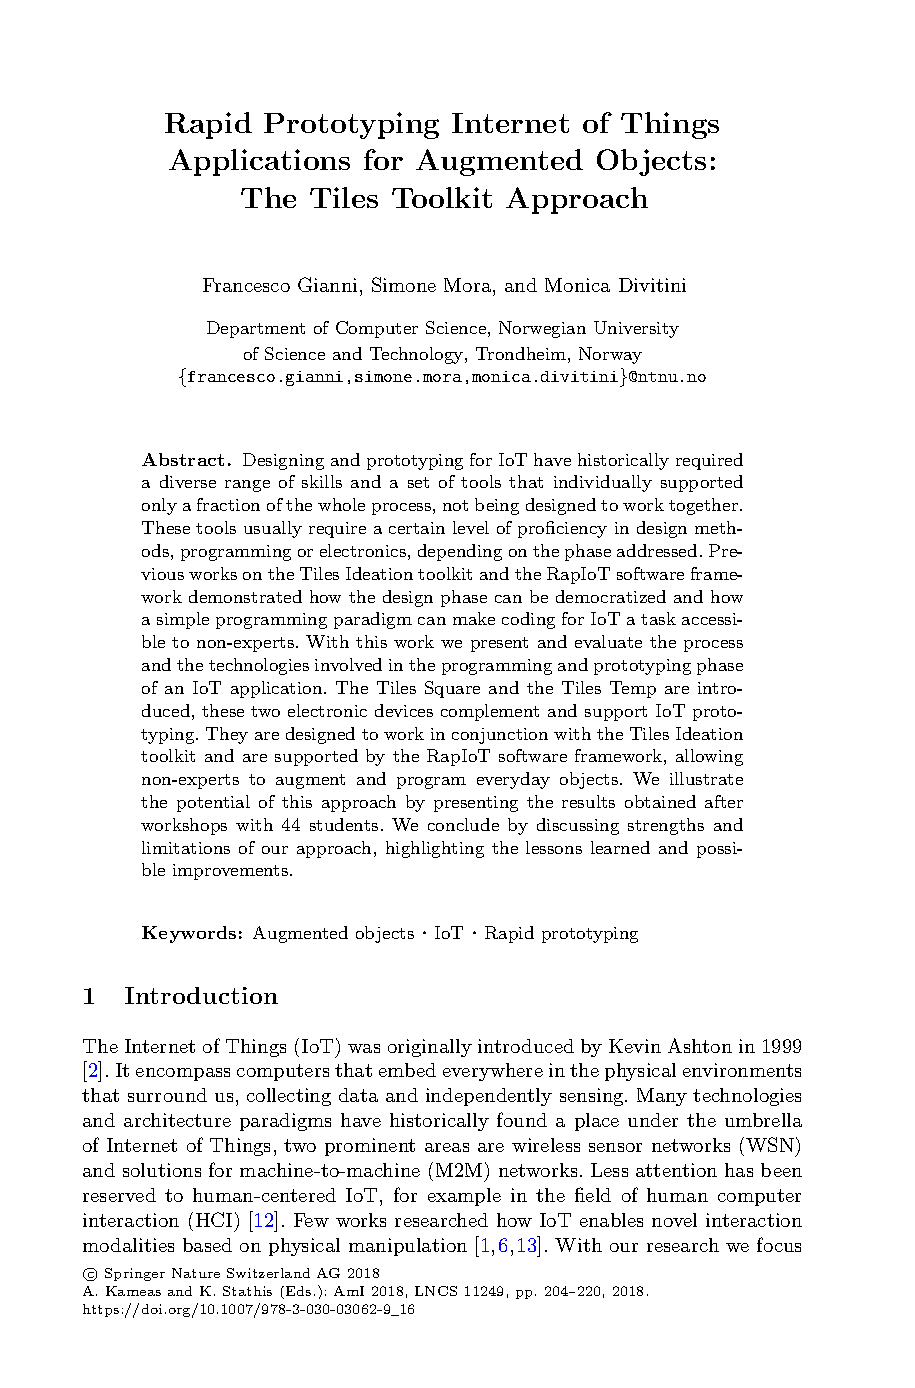
\includepdf[pages=-, noautoscale=true, scale=1, offset=7mm 0mm]{./papers_published/P7_thesis_edit.pdf}

\end{document}

%2019:185 	ISBN 978-82-326-3967-0 	Electronic 	2019-05-21
%2019:185 	ISBN 978-82-326-3966-3 	Printed 	2019-05-21
